% !TEX TS-program = pdflatex
% !TEX encoding = UTF-8 Unicode


\documentclass[a4paper, oneside, 
               justified=true, sfsidenotes]{tufte-book} 

\usepackage[utf8]{inputenc} % set input encoding to utf8
\usepackage[english]{babel}[2005/11/23]
\usepackage{phd}

%% Bibliography
\usepackage{natbib}
% useful to write files on the fly

\bibliographystyle{plainnat} % note the change here
\bibpunct{(}{)}{;}{a}{,}{,}


\usepackage{verbatim}
\usepackage{caption}
\DeclareCaptionFont{blue}{\color{black}\small}

\captionsetup{justification=raggedright, singlelinecheck=false,
                     font={blue,sf,small}}


%overwrite tufte and have numbering
\setcounter{secnumdepth}{5}


%% Change some of the looks
%%% CHAPTER STYLES AND SECTION STYLES
\pagestyle{fancy}
\renewcommand{\chaptermark}[1]%
{\markboth{\MakeUppercase{\chaptertitlename\ \thechapter\ #1}}{}} 
\renewcommand{\sectionmark}[1]%
{\markright{\MakeUppercase{\thesection~\ #1}}}
\renewcommand{\headrulewidth}{0.5pt}
\renewcommand{\footrulewidth}{0pt}
\newcommand{\helv}{%
\fontfamily{phv}\fontseries{b}\fontsize{9}{11}\selectfont}
\fancyhf{}
\fancyhead[LE,RO]{\helv \thepage}
\fancyhead[LO]{\helv \rightmark}
\fancyhead[RE]{\helv \leftmark}


% Typesets the font size, leading, and measure in the form of 10/12x26 pc.
\newcommand{\measure}[3]{#1/#2$\times$\unit[#3]{pc}}

% Macros for typesetting the documentation


\newcommand{\hlred}[1]{\textcolor{Maroon}{#1}}% prints in red

\newcommand{\hlmaroon}[1]{\textcolor{Maroon}{#1}}%print maroon


%\newcommand{\hangleft}[1]{\makebox[0pt][r]{#1}}




\newcommand{\hairsp}{\hspace{1pt}}% hair space
\newcommand{\hquad}{\hskip0.5em\relax}% half quad space
\newcommand{\TODO}{\textcolor{red}{\bf TODO!}\xspace}

\newcommand{\ie}{\textit{i.\hairsp{}e.}\xspace}
\newcommand{\eg}{\textit{e.\hairsp{}g.}\xspace}





% Generates the index we use before the
% out
\usepackage{makeidx}
\makeindex



%%% ACTIVITY DATES
%% Define a new command for activity key-dates
%% this can be saved for shipout later
\newcommand{\keydate}[2]{#1  #2 \\}
\newcommand{\out}[2]{%
  {\index{key dates!#1}% add to index
\immediate\write\tempfile{\noexpand\keydate{ #1}{#2}}}}


%% We open the file to  to write the key-dates
%% we will use it later to import
\newwrite\tempfile
\immediate\openout\tempfile=keydates.tex


\usepackage{fancyvrb}




%%% Set some local commands and colors
%\usepackage{colortbl}
%\definecolor{green}{rgb}{0.1,0.1,0.1}
%%\color{green!40!yellow})


\newcounter{sectionstep}
\setcounter{sectionstep}{0}

\def\tablesection{%
  \midrule
  \stepcounter{step}%
  \setcounter{sectionstep}{-1}%
  \setcounter{sectionstep}{-1}%
}

\def\Inc{%
  \stepcounter{sectionstep}%
\thestep.0\thesectionstep%
}


\makeatletter
\def\chapter{\clearpage\thispagestyle{plain}\global\@topnum
  \z@\@afterindentfalse
  \secdef\@chapter\@schapter
}
\makeatother


\title{CLOSURE \\AND\\COMMISSIONING\\PLAN FOR MEP}
\author{City Center Phase 3a \&3b}
\publisher{Habtoor Leighton Specon llc}
\date{January 2011} % Delete this line to display the current date

%\newcounter{step}
%\def\inc{\stepcounter{step}\thestep}

% shorthands for typing equipment numbers
% that make sense.
\def\panel#1{{\inc\space\space\small\texttt{#1}}}

\def\EI#1{\texttt{EI}}
\DeclareRobustCommand\refs[1]{\S\hskip0.5pt\ref{#1}}

\DeclareRobustCommand\WIR{{\Large\WritingHand}}


\usepackage[smaller,printonlyused,withpage]{acronym}

\usepackage{hyperref}
\hypersetup{%draft, % = no hyperlinking at all (useful in b/w printouts)
    colorlinks=true, linktocpage=true, pdfstartpage=1, pdfstartview=FitV,%
    % uncomment the following line if you want to have black links (e.g., for printing)
    %colorlinks=false, linktocpage=false, pdfborder={0 0 0}, pdfstartpage=3, pdfstartview=FitV,% 
linktocpage=true,  breaklinks=true, pdfpagemode=UseNone, pageanchor=true,  pdfpagemode=UseOutlines,%
    plainpages=false, bookmarksnumbered, bookmarksopen=true, bookmarksopenlevel=1,%
    hypertexnames=true, pdfhighlight=/O,hyperfootnotes=true,%nesting=true,%frenchlinks,%
    urlcolor=webbrown, linkcolor=RoyalBlue, citecolor=webgreen, %pagecolor=RoyalBlue,%
    %urlcolor=Black, linkcolor=Black, citecolor=Black, %pagecolor=Black,%
    pdftitle={Closure and Commissioning Plan},%
    pdfauthor={Dr Y Lazarides},%
    pdfsubject={City Center, report},%
    pdfkeywords={},%
    pdfcreator={pdfLaTeX},%
    pdfproducer={LaTeX with hyperref and classicthesis}%
} 
  
\let\ch\checkmark
\def\fire{{\LARGE\color{red}\Fire}}
\def\Danger{{\LARGE\color{red}\danger}}
\long\def\askar{\parbox{4cm}{\Danger \RaggedRight Askar condensers.}}

\begin{document}

% Front matter
\frontmatter

\maketitle
\tableofcontents
\listoffigures
\listoftables


\mainmatter


\cleardoublepage

\chapter*{Update}

Given the current constraints of the Project, we are satisfied that the general direction of the Project is doing well and we will be in a position to offer the works for Civil Defence Inspection at end of March and shortly thereafter to enable the Operators to take possession of the Hotels.

Physical installations in Towers and Podia have been completed in their majority and final fix activities are following the pace of both the Main Contractor as well as Fit-out activities. 

EIs, RFIs and other constraints have slowed down the works and obstructed a reasonable implementation of our original Closure and Commissioning Plan.

\section*{Objectives}

The aim of this report is to summarize the status of the works
and propose a reasonable plan for Closure of the Works and the implementation of a Commissioning Plan.

I general we are proposing a focus where areas can be fully completed, as well as the enabling of commissioning of all systems to take place. We suggest to start focusing on the
Shangri-la Hotel first, as this presents more difficulties.

\begin{longtable}{lll}
\toprule
Item  &Area   & Milestone \\
\midrule
\inc     & Podium Rotana    & 16 Feb 2013\\
\inc     & Tower Rotana     & 16 Mar 2013\\
\inc     & Podium Shangrila & 30 Jan 2013\\
\inc     & Tower Shangrila  & 15 Feb 2013\\
\inc     & Merweb Podium    & 17 Mar 2013\\
\inc     & Tower Merweb     & 30 Apr 2013\\
\bottomrule
\end{longtable}

We suggest a 4-7 week cycle for each Hotel at which point we expect that all physical works will close (including comments, FORs and NCRs) and the enabling of all systems to be commissioned. A small Team can remain to continue closing any issues that arise out of these activities and to follow-up on activities delayed by the Fit-out subcontractor.

Within Podia the following sequence is preferred, whereas in the Towers a top to bottom sequence will be followed.

\begin{table}[htbp]
\centering
\begin{tabular}{ccc}
\toprule
Item  &Area   & Milestone \\
\midrule
1     & B1 & 20 Jan\\
2     & B3 & 20 Jan \\
3     & B2 & 20 Jan \\
4     & L6 & 20 Jan\\
5     & L4 & 27 Jan\\
6     & L3 & 27 Jan\\
7     & L7 &  5 Feb\\
8     & L2 & 10 Feb\\
9     & L1 & 10 Feb\\
10    & L5 & 10 Feb\\
11    & GF & 20 Feb\\
\bottomrule
\end{tabular}
\caption{Floor sequence of works.}
\end{table}

Sequence as shown is not that important and the logic behind it, is to enable other trades, such as Dragoni to complete the
works before concentrating in the area. Also we expect the CCTV
changes to affect these areas and we prefer to work in them
once all the other areas are completed.

More details can be found in the relevant area and system sections of the report.


\section{Personnel}


 Table~\ref{tbl:manpower} summarizes the manpower currently on the Project. 

\def\Z{\phantom{Z}}
\begin{table}[htbp]
\begin{center}
\begin{tabular}{l r r}
\toprule
Company           &Tradesmen   & Tradesmen\\
~                 &30 January  & 30 March \\
\midrule
Specon            &503         & 681\\
Al-Jaber          &181         &182\\
Crompton          &0           &59\\
QMMC              &112         &113\\
Nafco             &5           &16\\
ERE               &10          & 0\\
                  &\underline{\phantom{1075}}
                  &\underline{\phantom{1075}}\\
Subtotal          &912         &1201\\

Hired manpower    &            &\\
\Z ERE            &10          & nil\\

                  & \underline{\phantom{1075}}
                  & \underline{\phantom{1075}}\\
\Z Total hire manpower &127     &137\\
~&&\\
Total                      & \underline{\underline{1039}}       &\underline{\underline{1338}}\\
                             & &\\
\bottomrule
\end{tabular}
\caption{Average Manpower as of January 2013}
\label{tbl:manpower}
\end{center}
\end{table}



\section*{Current Constraints affecting completion}

\begin{enumerate}
\item Disruption due to Commercial issues.
\item Continued disruption with EIs and other changes.
\item Premature demobiliziation and large number of personnel resigning.
\item Demobilization of Al-Jaber due to Commercial issues.
\item Slow down by all sub-contractors due to commercial issues.
\item Fire Protection
\item Imbalances in resources between the Main Contractor, MEP Subcontractors and Finishing Contractor. This needs to be addressed in order to be able to improve on our completion projections.
\end{enumerate}

\section*{Demobilization}

We have experienced higher than normal attrition of staff and technicians. 

\section*{Recommendations}
Our recommendation is to focus our attention and resources on a Tower by Tower rather than spreading technicians over the full extend of the works.




\chapter{Civil Defence Approval}
\parindent1em
\label{civildefence}

\begin{update}
\centerline{\textbf{Update 23 April 2013}}

\noindent MEP related activities are expected to be completed by 30 April 2013 or thereabouts with the exceptions described later on and as described in the Executive Summary of the report. The difficult areas of Smoke Tests and Fire Alarm are expected to be completed, with minor deviations. Clearing of comments and WIRs will be issued after the 30 April and are expected to take 10-15 days to clear, budgeting time for the inefficiencies of the WIR process and the necessity to carry out workshops. We are confident that 
an appointment can be sought for the CDD Inspection for the 30 May 2013 as planned.

\end{update}

Civil Defence Inspections can only take place when the Building Operations have been completed, when the full Fire Fighting,  Fire Alarm, Staircase Pressurization and Smoke Exhaust systems have been completed tested and commissioned. We expect that this will only be possible at the earliest by end April  2013. However, we will re-evaluate these dates once the works progress a bit further. 


The Qatar Civil Defence Department if approached can unofficially inspect the works earlier in order to identify problem areas earlier. However, at this stage it is bound to catch rather known problems than unknown problems.

The Civil Defence related sections have been discussed under separate headings and will not be repeated here. See \tref{cdd} for status and details.


\begin{table}[h]
\begin{tabular}{lr}
\toprule
\textbf{Description}	 &\textbf{Qty}\\
\midrule 	 
\textbf{Fire Fighting System}	 &\\
Sprinkler Points	    &26,078\\
Fire Hose Cabinets	    &457 \\
Zone Control Valves	    &393 \\
Pressure Reducing Valves	 &288 \\
Breeching Inlets	        &3\\ 
Fire Hydrants	            &13\\ 
OS\&Y Valves	               &86\\ 
\textbf{Alarm Check Valves}	              &18 \\
Check Valves / Non Return Valves &18 \\
Fire Extinguishers Dry Powder	 &691 \\
Fire Extinguishers CO2	           &457 \\
Fire Pumps	                     &12 \\
Jockey Pumps	                     &6 \\
\midrule 	 
\textbf{Fire Alarm System}	 &\\
Smoke \& Heat Detectors	 &7,573 \\
Monitor / Control Modules	       &2,252 \\
Sounders / Speakers / Voice Evacuation	   &2,630 \\
Main Fire Alarm Control Panel	         &9 \\
Conventional Fire Alarm Panel	        &16 \\
Voice Evacuation Panel	                  &9 \\
\midrule 
\textbf{FM200 System}	 &\\
Fire Extinguisher Control Panel	&36 \\
FM200 Cylinder with Agent	            &38 \\
\midrule 	 
\textbf{Foam System}	 &\\
Deluge Valve with complete trimming	 &2 \\
Bladder Tank	                        &2 \\
Foam Chemical	                   &100 Gal\\
\bottomrule
\end{tabular}
\caption{Items comprising the Fire Protection System}
\label{fireitems}
\end{table}

\tref{fireitems} lists all the devices related to Fire Life Safety code requirements and indicates clearly the extend of the challenge to complete the installation and commissioning within the stipulated time. Terminal devices are still to be installed in Merweb and a great number of them are still to be delivered. Of special concern are the large number of devices related to the Fire Alarm system (approximately 13,000) which are prone to errors and false alarms.




\medskip

\captionof{table}{Summary CDD requirements.}
\label{cdd}
{\small\RaggedRight
\begin{longtable}{p{2.3cm}p{4.2cm}p{4.2cm}}

\toprule
Fire Protection    &Firefighting system.  & Ready except 2 rooms\\
        &Fire suppression FM~200 system. & 90\%\\
	&Fire alarm \& voice evacuation system. & 90\%\\
	&Fire alarm control rooms. & 97\%\\
	&Fire Water tanks & \Danger Expected Completion 20 Mar 2013. We will fill on the 30 April 2013. \\
	&Evacuation Map & HLG Scope\\
	&FA Matrix & Submitted\\
	&Life Safety \& fire protection cause and 
         effect report & \ch\\
	&Function \& Sequence of operation & On-going\\
\midrule

HVAC	&Staircase Pressurization System & Merweb Testing 23 April 2013\\
	&ECUs, SEF, EAF, AHU, FAF, ECU, SMD, FD etc… &\\
	&Car Park Ventilation & See \S\ref{carparkventilation}\\
	&Function \& sequence of operation & As above\\
\midrule


Electrical	&Exit \& emergency lights. & Completed\\
	&Power Diesel generator \& ATS. & Partially completed\\
	&DG Tanks. & Not available (Client Scope).\\
	&Access control system.  & 15 May 2013\\
	&CPMS. & Tested Internally\\
	&UPS system. & See \refs{ups}, Completed\\
	&Lift sequence of operation & Physical Installation completed, Awaiting Kone to Test.\\
\midrule

Documents	&Drawings &\\
	& Method Statements &\ch \\
	& Sequence of operation &\ch \\
	& Products certificates &\ch \\
	& T\&C reports, &\\
	& Undertaking letter to CDD &\\
	& Certificate of HLG \& NAFFCO &\\
        & Certificate Al-Misnad              &\ch 9 Mar 2013\\
	&MEP Function \& sequence of operation manual/Report, Interface \& Integrity reports &ongoing\\
	&Stamped \& approved Shop Drawing &\ch \\
\bottomrule
\end{longtable}
}

\section{Civil Defence Inspection Checklist base on Phase II Inspection}

Comments that need action based on Phase II inspection.



\begin{table}[htbp]
\resetinc
{\RaggedRight\small
\begin{tabular}{p{0.5cm}p{4.5cm}ll}
\toprule
item  & Activity  & Status  & Remarks\\
\midrule
\inc & Fire exit staircase identification, inside stair floor with clear identification marking, "TO BASEMENT NO EXIT", "NO ROOF ACCESS" signages etc. & & 30 Mar 2013\\
\inc & Identification marking for mechanical rooms, fire pump room, electrical room, Fire Lift, Fire Command Center and other important building/services rooms. && 30 Mar 2013\\
\inc & "In Case of Fire Do not Use Lift" in arabic identification marks fro mechanical room, fire pump room, exit staircases, exit access routes, as per NFPA 101            &&30 Mar 2013\\
\inc & Label marking for all access doors for Fire Dampers & &30 Mar 2013\\

\bottomrule

\end{tabular}}
\caption{Emergency Lights, signs and markings. Works under HLG.}
\end{table}








\chapter {Fire Alarm}
\label{firealarm}
\newthought{Perhaps the most critical system} that affects the Civil Defence Inspection is the completion and Commissioning of the Fire Detection System. The system has now advanced to comissioning stage for most of the Tower areas and Podia.

\hl{A meeting took place with the Supplier, who advised that Fire Ventilation Panels have been delayed and  are estimated to arrive to Doha on the 15 Apr 2013. A method was agreed to minimize the impact on the works. We also received part of the outstanding orders.}

\begin{marginfigure}
\includegraphics[width=\linewidth]{../pic/FC-002}
\caption{Fire Control rooms are ready for all Towers (missing Fire Control Panels) are expected to arrive on the 15 Mar 2013}
\end{marginfigure}


%ROTANA
\captionof{table}{Status of Fire Alarm Works in Rotana.}
\begin{longtable}{cp{3cm}ccp{2.8cm}}
\toprule
Level & Item & Inst. & T\&C &Remarks\\
\midrule
L45   & BPS       &\checkmark         &\checkmark          &            \\
L41   & BPS       &\checkmark         &\checkmark          &            \\
L40   & APS       &\checkmark         &\checkmark          &            \\
L33   & APS       &\checkmark         &\checkmark          &            \\
\midrule
L28   & APS           &\checkmark        & \checkmark         &         \\
        & FACP2       &\checkmark         & \checkmark         &         \\
        & VACP1       &\checkmark         &\checkmark          &         \\
        & VACP2       &\checkmark         & \checkmark         &         \\
\midrule
L23   & BPS       &\checkmark         & \checkmark         &            \\
L21   & APS       &\checkmark         &\checkmark          &            \\
L19   & BPS       &\checkmark         &\checkmark          &            \\
L15   & APS       &\checkmark         &\checkmark          &            \\
        & APS       &\checkmark         & \checkmark         &            \\
\midrule
L8	& APS       &\checkmark         &\checkmark          &            \\
        &FACP1    & \checkmark                          &\checkmark        &            \\
        &VACP2    &  \checkmark                         &\checkmark        &            \\
\midrule
\textbf{GL}    &             &                                    &        &\\
       & BPS       &                                    &       &Awaiting delivery\\ 
       & MFACP   & \checkmark                  & & \\
       & MVACP1 & \checkmark                  & &\\
       & MVACP2 & \checkmark                  & &\\
       & Graphic Command Center PC  &     & &\\
       & System Printer                      &\checkmark     &&\\
       &back-up battery cabinet           & \checkmark    &&\\
       &smoke panel                          &                      & & Awaiting delivery\\
       &RCA-Front-desk                      &                      & &Front desk not ready\\
       &RCA-back desk                       &                      & &                             \\
       &RCA-operator room                &                      & &                             \\
       &RFACP-fire control room (mimic panel)        &\checkmark                      & &        \\
      &RFACP Eng. Room                   &                 &                                      &\\
      &RCA-GM Office Room               &                &                                      &\\
\midrule
B3	&BAPS       &\checkmark         &          &            \\
        &conventional FACP                &\checkmark         &            \\
        &conventional FACP                &\checkmark         &            \\
 \bottomrule
\end{longtable}

%SHANGRILA

{\RaggedRight\small
\captionof{table}{Status of Fire Alarm Works in Shangrila.}
\begin{longtable}{lp{3cm}llp{2.8cm}}

\toprule
Level & Item & Inst. & T\&C &Remarks\\
\midrule
L47   & BPS       &\checkmark         & \checkmark         &            \\
L43   & BPS       &\checkmark         & \checkmark         &            \\
L40   & APS       &\checkmark         & \checkmark         &            \\
L40   & APS       &\checkmark         &\checkmark          &            \\
L39   & BPS       &\checkmark         & \checkmark         &            \\
L33   & APS           &\checkmark        & \checkmark         &            \\
L27   & APS           &\checkmark        & \checkmark         &            \\
\midrule

L1        & FACP2       &\checkmark         &\checkmark          &            \\
        & VACP1       &\checkmark         &\checkmark          &            \\
        & VACP2       &\checkmark         & \checkmark         &            \\
\midrule
L8   & APS       &\checkmark         & \checkmark         &            \\
\midrule
\textbf{GL}    &             &                                    &        &\\
       & BPS       &                                    &       &Awaiting delivery\\ 
       & MFACP   & \checkmark                  & & \\
       & MVACP1 & \checkmark                  & &\\
       & MVACP2 & \checkmark                  & &\\
       & Graphic Command Center PC  &     & &\\
       & System Printer                      &\checkmark     &&\\
       &back-up battery cabinet           & \checkmark    &&\\
       &smoke panel                          &                      & & Awaiting delivery\\
       &RCA-Front-desk                      &                      & &Front desk not ready\\
       &RCA-back desk                       &                      & &                             \\
       &RCA-operator room                &                      & &                             \\
       &RFACP-fire control room (mimic panel)        &\checkmark                      & &        \\
      &RFACP Eng. Room                   &                 &                                      &\\
      &RCA-GM Office Room               &                &                                      &\\
\midrule
B3	&BAPS       &\checkmark         &          &            \\
        &conventional FACP           &\checkmark         &\checkmark            \\
        &conventional FACP           &\checkmark         & \checkmark           \\
 \bottomrule

\end{longtable}}

\section{Outstanding material orders}
Oustanding material orders have been held-up due to delays in amending the L/C. Table\ref{faorders} shows the outstanding deliveries.
\vspace*{1cm}

\captionof{table}{Outstanding Material Orders}
\label{faorders}
\resetinc
\begin{longtable}{ll rl}
\toprule
Sn & Order         & Amount (QR)   & Remarks\\
\midrule
\inc & EL-0022-2 & 202, 107   & \\
\inc & EL-0023-2 & 119,118  & \\
\inc & EL-0277   &6,800  &\\
\inc & EL-0422   & 76,087 &\\
\inc & EL-0433   & 205,727 &\\
\inc & EL-0433-1  &3,275&\\
      &                &\ul{~~~~~~}&\\
      &                & 613,115\\
\bottomrule
\end{longtable}















\chapter{Fire Fighting}
\index{FireFighting! General}


\newthought{The Fire Protection System} has been substantially
completed with the exception of where ceilings have not been completed. These areas include vestibules in Towers, some lift lobbies in podia and droppers into walk-in cold stores. The
Plantroom has been energized and tested, as well as the majority of the rest of the network, including Towers. The extend of the system is detailed in \tref{fireitems}.

\begin{figure*}
\includegraphics[width=\linewidth]{./pic/F-001}
\caption{All items for the Fire Plantrooms are ready. The systems have been pre-commissioned and
switched on. Main constraint remaining is teh completion of internal plantforms in tanks.}
\end{figure*}
 

\section{Current Detailed Status and Targets}

The current status is shown in Tables \ref{tbl:fire1}, \ref{tbl:fire2} and \ref{tbl:fire3}. We are now in the process of submitting official WIRs for commissioning. Repair works on Rotana Tower have been completed and we currently working on an overtime basis to complete them on Shangrila. On Merweb the work is undertaken by AJE. The sprinkler status is shown in Table. Unfortunately final fix items cannot be completed until all vestibules and other finishing related items are completed.

\begin{table}[htbp]\label{tbl:fire1}
\begin{center}
\begin{tabular}{lllll}
\toprule
\multicolumn{5}{c}{Rotana}\\
\midrule
Level	&Risers    &ZCV	      &FHC  &Target\\
\midrule
B3	&\checkmark     &\checkmark	 &\checkmark  &\\
B2	&\checkmark     &\checkmark	 &\checkmark  &\\
B1	&\checkmark     &\checkmark	 &\checkmark  &\\
GL	&\checkmark     &\checkmark	 &\checkmark  &\\
L1	&\checkmark     &\checkmark	 &\checkmark  &\\
L2	&\checkmark     &\checkmark	 &\checkmark  &\\
L3	&\checkmark     &\checkmark	 &\checkmark  &\\
L4	&\checkmark     &\checkmark	 &\checkmark  &\\
L5	&\checkmark     &\checkmark	 &\checkmark  &\\
L6	&\checkmark     &\checkmark	 &\checkmark  &\\
L7	&\checkmark     &\checkmark	 &\checkmark  &\\
\midrule
L8-14 &\checkmark     &\checkmark	 &\checkmark  &\\
L15	&\checkmark     &\checkmark	 &\checkmark  &\\ 	 
L16-38	&\checkmark     &\checkmark	 &\checkmark  &\\	 	 
L39-47	&\checkmark     &\checkmark	 &\checkmark  &\\	 	 
\bottomrule
\end{tabular}
\caption{Rotana Risers, zone valves and FHC completion status.}
\end{center}
\end{table}

\begin{table}[htbp]\label{tbl:fire2}
\begin{center}
\begin{tabular}{lllll}
\toprule
\multicolumn{5}{c}{Shangri-la}\\
\midrule
Level	&Risers &ZCV	&FHC  &Target\\
\midrule
B3	&\checkmark     &\checkmark	 &\checkmark  &\\
B2	&\checkmark     &\checkmark	 &\checkmark  &\\
B1	&\checkmark     &\checkmark	 &\checkmark  &\\
GL	&\checkmark     &\checkmark	 &\checkmark  &\\
L1	&\checkmark     &\checkmark	 &\checkmark  &\\
L2	&\checkmark     &\checkmark	 &\checkmark  &\\
L3	&\checkmark     &\checkmark	 &\checkmark  &\\
L4	&\checkmark     &\checkmark	 &\checkmark  &\\
L5	&\checkmark     &\checkmark	 &\checkmark  &\\
L6	&\checkmark     &\checkmark	 &\checkmark  &\\
L7	&\checkmark     &\checkmark	 &\checkmark  &\\
\midrule
L8-14	&\checkmark     &\checkmark	 &\checkmark  &\\
L15	&\checkmark     &\checkmark	 &\checkmark  &\\	 	 
L16-38	&\checkmark     &\checkmark	 &\checkmark  &\\ 	 
L39-L47	&\checkmark     &\checkmark	 &\checkmark  &\\ 	 	 
 \bottomrule
\end{tabular}
\caption{Shangrila Risers, zone valves and FHC targets}
\end{center}
\end{table}

\begin{table}[htbp]\label{tbl:fire3}
\begin{center}
\begin{tabular}{lllll}
\toprule
\multicolumn{5}{c}{Merweb}\\
\midrule
Level	&Risers &ZCV	&FHC  &Target\\
\midrule
B3	&\checkmark     &\checkmark	 &\checkmark  &\\
B2	&\checkmark     &\checkmark	 &\checkmark  &\\
B1	&\checkmark     &\checkmark	 &\checkmark  &\\
GL	&\checkmark     &\checkmark	 &\checkmark  &\\
L1	&\checkmark     &\checkmark	 &\checkmark  &\\
L2	&\checkmark     &\checkmark	 &\checkmark  &\\
L3	&\checkmark     &\checkmark	 &\checkmark  &\\
L4	&\checkmark     &\checkmark	 &\checkmark  &\\
L5	&\checkmark     &\checkmark	 &\checkmark  &\\
L6	&\checkmark     &\checkmark	 &\checkmark  &\\
L7	&\checkmark     &\checkmark	 &\checkmark  &\\
\midrule
L8-14	&\checkmark     &\checkmark	 &\checkmark  &\\
L-15	&\checkmark     &\checkmark	 &\checkmark  &\\
L16-38	&\checkmark     &\checkmark	 &\checkmark  &\\
L39-47	&\checkmark     &\checkmark	 &\checkmark  &\\
\bottomrule
\end{tabular}
\caption{Merweb Risers, zone valves and FHC targets}
\end{center}
\end{table}

\section{Helipad Foam Installations}

The helipad foam installations---have been completed by HLS---as Nafco failed to complete. There is still a missing part (hydraulic valve) and the foam still needs to be delivered to Site. Upon completion of the above we estimate that we can commission the system within 2-3 days. The system is best to be commissioned in the presence of the Helipad Supplier.



\section{Constraints}

We summarize the current constraints in achieving the target completion date as below:
\medskip

{\RaggedRight
\begin{tabular}{lp{3.5cm}ll}
\toprule
Item    & Detail  & Action &Date \\
\midrule
\inc &Completion of Water Tank platforms and water tanks. &HLG & 28 Feb 20013\\
\inc &Completion of vestibule areas by Dragoni. &Dragoni & Unknown \\
\inc &Completion of other areas under Dragoni scope. &Dragoni & Unknown\\
\bottomrule
\end{tabular}}
\medskip

We are of the opinion that risks remain in the areas not under our control or that of HLG.

\begin{table}[htbp]
\begin{tabular}{lr}
\toprule
\textbf{Description}	 &\textbf{Qty}\\
\midrule 	 
\textbf{Fire Fighting System}	 &\\
Sprinkler Points	    &26,078\\
Fire Hose Cabinets	    &457 \\
Zone Control Valves	    &393 \\
Pressure Reducing Valves	 &288 \\
Breeching Inlets	        &3\\ 
Fire Hydrants	            &13\\ 
OS\&Y Valves	               &86\\ 
\textbf{Alarm Check Valves}	              &18 \\
Check Valves / Non Return Valves &18 \\
Fire Extinguishers Dry Powder	 &691 \\
Fire Extinguishers CO2	           &457 \\
Fire Pumps	                     &12 \\
Jockey Pumps	                     &6 \\
\midrule 	 
\textbf{Fire Alarm System}	 &\\
Smoke \& Heat Detectors	 &7,573 \\
Monitor / Control Modules	       &2,252 \\
Sounders / Speakers / Voice Evacuation	   &2,630 \\
Main Fire Alarm Control Panel	         &9 \\
Conventional Fire Alarm Panel	        &16 \\
Voice Evacuation Panel	                  &9 \\
\midrule 
\textbf{FM200 System}	 &\\
Fire Extinguisher Control Panel	&36 \\
FM200 Cylinder with Agent	            &38 \\
\midrule 	 
\textbf{Foam System}	 &\\
Deluge Valve with complete trimming	 &2 \\
Bladder Tank	                        &2 \\
Foam Chemical	                   &100 Gal\\
\bottomrule
\end{tabular}
\caption{Items comprising the Fire Protection System}
\label{fireitems}
\end{table}


%\clearpage
%
%\begin{tikzpicture}[scale=1.15]
%\begin{ganttchart}[vgrid,hgrid,x unit=3.5mm,
%   y unit chart=3.5mm, bar height=0.5, bar label font=\footnotesize,
%   ]{24}
%\gantttitle{Fire Fighting, FHC, HD and Sprinkler System \vbox{2012}}{24} \\
%\gantttitlelist{1,...,24}{1} \\
%\activity[purple]{Merweb Tower}{1}{12}
%\activity[purple]{Merweb Podium}{1}{8}
%\activity[violet]{Rotana Tower}{1}{6}
%\activity[violet]{Rotana Podium}{1}{7}
%\activity[violet]{Shangri-la Tower}{1}{6}
%\activity[violet]{Shangri-la Podium}{1}{7}

%\ganttbar{Water Tanks Testing}{1}{2} \\
%\activity[purple]{Overall pressure test}{3}{7} \ganttnewline
%\ganttmilestone[milestone={fill=purple}]{Milestone}{7} \ganttnewline
%\ganttbar[bar={fill=orange, draw=none}]{Final Task}{8}{12}\\
%\ganttlink{elem2}{elem3}
%\ganttlink{elem3}{elem4}
%\activity{Pump alignment}{5}{1}
%\activity{Circulate to towers}{6}{}
%\activity{Controls}{7}{}
%\activity{HX Commissioning}{7}{1}
%\activity{Disinfection}{8}{1}
%\activity{Flush}{9}{10}
%\activity{Set to operation}{9}{10}
%\end{ganttchart}
%\end{tikzpicture}




\chapter{Staircase Pressurization}



\begin{marginfigure}
  \includegraphics[width=\linewidth]{rusting}
  \caption{fans showing signs of corrossion}
  \label{fig:rusting}
\end{marginfigure}

\newthought{The Staircase Pressurization} systems are expected to be completed by the 15 February 2012. Physical works have been completed and commissioning has started.

           \begin{margintable} 
	    \begin{tabular}{lcl}
	      \toprule
	      System    & Key Milestone Date  \\
	      \midrule
                 Rotana      & $15^{th}$  January 2012  \\   
                 Shangri-la  & $30^{th}$ January 2012\\
	     Merweb     &  $15^{th}$  February 2012  \\
     	      \bottomrule
	    \end{tabular}
           \caption{Staircase Pressurization Key Dates}
           \label{tbl:KEkeydates}
            \end{margintable}
\index{Key Dates!Rotana staircase pressurization system}
\index{Key Dates!Merweb staircase pressurization system}
\index{Key Dates!Shangrila staircase pressurization system}

\section{Current Status}

All plant-room level fans have been installed and have been
inspected.



\section{Constraints}


\begin{enumerate} 
\item Some grilles missing in Merweb.
\item All doors need to be installed and completed.
\end{enumerate}

\section{Commissioning Organization}


The work has been subdivided for convenience as follows:

   \begin{table}[htbp] 
	    \begin{tabular}{l p{4cm}l}
	      \toprule
	     Item & Cut-off date  \\
	      \midrule
                  1 &Rotana & \lambros \\
                  2 &Shangrila &\sotiris \\
	      3  &Merweb  & \sotiris  \\
                 4  &All electrical &\NH\\
                   \bottomrule
	    \end{tabular}
           \caption{Staircase Pressurization responsible persons}
            \end{table}














\newcommand{\keextracton}{25.10.2010}
\newcommand{\ecolon}{25.10.2010}           % ecological units on
\newcommand{\podiumon}{26.10.2010}
\newcommand{\toweron}{15.10.2010}
\newcommand{\kdpoweron}{20.10.2010}

\chapter{Kitchen Extract Ventilation System }
%\begin{marginfigure}
%  \includegraphics[width=\linewidth]{boilers}
 % \caption{Calorifier plant-room in Merweb.}
 % \label{fig:marginfig1}
%\end{marginfigure}

\newthought{The Kitchen Extract System} has been physically completed with the exception of final connections to hoods, where the Direct Owner's Subcontractor has not as yet installed the extract canopies.  Final connections to stainless steel fans and some ducting is still to be completed for some areas.\sidenote{These works were contracted out to QMMC, who failed to complete. HS has now taken action to complete the works.} Commissioning has started on ECUs.

\out{Rotana kitchen extract}{25 Feb 2013}
\out{Shangri-la kitchen extract}{15 Mar 2013}
\out{Merweb kitchen extract}{30 Mar 2013}


           \begin{margintable} 
	    \begin{tabular}{lcl}
	      \toprule
	      System    & Key T\&Milestone Date  \\
	      \midrule

              Rotana Kitchen Extract       &  25 Feb 2013  \\   
              Shangri-la Kitchen Extract   & 15 Mar 2013\\
	     Merweb Kitchen Extract       &  30 Mar 2013  \\
	      
	      \bottomrule
	    \end{tabular}
           \caption{Kitchen Extract Ventilation Key Dates (ECU)}
           \label{KEkeydates}
            \end{margintable}
 

\section{Current Status}

The kitchen extract system is made up of a series of black steel ductwork, extract fans and Ecological Units. The latter treat the air to  remove odours and contaminants, so as to enable the discharge of air at lower levels than the roof of the Towers. Most of the units are at Level~6, whereas the main kitchens are at Basement~1. 

The Ecological Units have been installed,  electrically connected and pre-tested with temporary power. As they are fed from the UPS, final testing will be done after the UPS final commissioning.\sidenote{Spare filters still to be ordered.}  

\section{Constraints}

Askar has to finalize installation of all kitchen hoods to enable the units to be fully commissioned.

\newenvironment{activitytable}{
\begin{longtable}{@{} c  l  l  l l  l l  p{3cm} }
\toprule
Floor/Activity &\textcircled{1}&\textcircled{2}
                   &\textcircled{3}&\textcircled{4}
                   &\textcircled{5}&\textcircled{\color{black}{6}}&Remarks\\
\midrule}{%
\bottomrule
\end{longtable}}

\section{Stainless steel works}

Stainless steel ductwork is being installed to serve kitchen dish-washing equipment and laudry exhausts. 
These works have been subcontracted to QMMC. They are currently behind schedule for insulation. 


\setcounter{step}{0}
\captionof{table}{Rotana, status of  works for stainless steel extract ductwork.\textcircled{1} ducting installation, \textcircled{2} insulation, \textcircled{3} fan installation, \textcircled{4} fan connection, \textcircled{5} electrical, \textcircled{6} Testing and Commissioning.}
\begin{activitytable}
7    &\panel{L7-RO-EF3} &\checkmark&\checkmark&\checkmark&& &pieces+fan conn.\\

6    &\panel{L6-RO-EF6} &&&& && EI not complete\\

5    &\panel{L5-RO-EF4} &\checkmark&\checkmark& \checkmark& &&insulation+elect\\

4   &&&&&&&\\

3    &\panel{L3-RO-EF4} &&&&&& EI\\

2    &&&&&&&\\

1    &\panel{L1-RO-EF2} &\checkmark&\checkmark &\checkmark&\checkmark&& final connection + insulation\\
1    &\panel{L1-RO-EF3} &\checkmark&\checkmark &\checkmark&& &final connection + insulation+client scope\\
1    &\panel{L1-RO-EF5} &&  &&&& reroute ducting\\


GF  &\panel{RO-GR-EF5} &\checkmark&\checkmark&\checkmark&\checkmark&&Final + some insulation (riser)\\
GF  &\panel{RO-GR-EF6} &\checkmark&\checkmark&\checkmark&\checkmark&& Final connection\\

B1  & &&&&&&\\

B2  & &&&&&&\\

B3  & &&&&&&\\
\end{activitytable}



\setcounter{step}{0}
\captionof{table}{Shangrila, status of  works for stainless steel extract ductwork. \textcircled{1} ducting installation, \textcircled{2} insulation, \textcircled{3} fan installation, \textcircled{4} fan connection, \textcircled{5} electrical, \textcircled{6} Testing and Commissioning.}
\begin{activitytable}
7    &\panel{L3-SL-EF4} &\checkmark&\checkmark&&&&snags+hood\\

6    &\panel{L3-SL-EF1}&&&&&& EI\\

5    &\panel{L3-SL-EL3} &\checkmark&\checkmark&\checkmark&\checkmark&&snags+hood\\

3   &\panel{L3-SL-EL4} &\checkmark&\checkmark&\checkmark&\checkmark&& snags+hood \\
     &\panel{L3-SL-EF9} &&&&&& EI-821 \\

2    & &&&&&&\\

1    &\panel{L1-SL-EF3} &\checkmark&\checkmark&\checkmark&&& snagging\\
1    &\panel{L1-SL-EF4} &---&---&\checkmark&---&& Dragoni scope\\

GF  &\panel{GR-SL-EF6} &\checkmark&\checkmark&\checkmark&\checkmark&& snagging+hood\\

B1  &\panel{B1-SL-EF8} &&&\checkmark&&& EI ducting express laundry\\
B1  &\panel{B1-SL-EF9} &\checkmark&\checkmark&\checkmark&&& +electrical\\


B2  & &&&&&&\\

B3  & &&&&&&\\
\end{activitytable}



\setcounter{step}{0}
\captionof{table}{Merweb, status of  works for stainless steel extract ductwork. \textcircled{1} ducting installation, \textcircled{2} insulation, \textcircled{3} fan installation, \textcircled{4} fan connection, \textcircled{5} electrical, \textcircled{6} Testing and Commissioning.}
\begin{activitytable}
7    & &&&&&&\\

6    & &&&&&&\\

5    &\panel{L5-MW-AF2} &\checkmark &\checkmark &\checkmark &\checkmark&& hood conn. + pieces\\
4    & & & & &&&\\
3    &\panel{L3-MW-AF5} &\checkmark&\checkmark&\checkmark&\checkmark&&hood conn.\\

2    & &&&&&&\\

1    &&&&&&&\\


GF  & &&&&&&\\

B1  & &&&&&&\\

B2  &&&&&&&\\

B3  &\panel{B3-MW-AF1} &\checkmark&&\checkmark&&&No ele.\\
     &\panel{B3-MW-AF2} &\checkmark&&\checkmark&&&\\
\end{activitytable}


\newenvironment{ECUtable}{
\begin{longtable}{@{} c  c  c  l l  l l  p{3cm} }
\toprule
Floor/Activity &\textcircled{1}&\textcircled{2}
                   &\textcircled{3}&\textcircled{4}
                   &\textcircled{5}&\textcircled{\color{black}{6}}&Remarks\\
\midrule}{%
\bottomrule
\end{longtable}}

\setcounter{step}{0}
\captionof{table}{Rotana, status of  works for stainless steel extract ductwork.\textcircled{1} Tag \textcircled{2} installation, \textcircled{3}hood connection, \textcircled{4}electrical, \textcircled{5} bms, \textcircled{6} Testing and Commissioning.}
\begin{ECUtable}
L7  &L7-RO-ECU-1 &Pool Kitchen& \checkmark &\checkmark &\checkmark&&\\
L6 & L6-RO-ECU-1 &Teatro&\checkmark&&&&\\
    & L6-RO-ECU-2 &Main Kitchen&\checkmark&&&&\\
    & L6-RO-ECU-4 &Boston Bar&\checkmark&&&&\\
L5 & n/a                &&&&&&\\
L4 & n/a                  &&&&&&\\
L3 & n/a                  &&&&&&\\
L2 & n/a                  &&&&&&\\
L1 & L1-RO-ECU-1   &All Day&\checkmark&&&&\\
    & L1-RO-ECU-2    &Lebanese&\checkmark&&&&\\
GF & GR-RO-ECU-1   &Banquet&\checkmark&&&&\\
B1 & n/a                  &&&&&&\\
B2 & n/a                  &&&&&&\\
B3 &  n/a                 &&&&&&\\
\end{ECUtable}

Other issues: mock-up of drain point, ordering balance, payment.




\chapter{Chilled Water System}
\index{Chilled Water Plantrooms}
\normalsize
%\begin{comment}
%\begin{marginfigure}%
%  \includegraphics[width=\linewidth]{rusting}
%  \caption{Equipment show eveidence of corrosion and neglect. Starting these equipment can present problems. Spares %need to be sourced as early as possible.(\url{http://asymptote.sf.net/}).}
 % \label{fig:marginfig1}
%\end{marginfigure}
%\end{comment}

\newthought{Chilled Water Plantrooms}  have been physically completed, pre-commissioned, part-commissioned and put into operation, in order to remove the temporary wild air installations, which were removed in October 2011.

\section{Basement Qatar Cool Plantrooms}
\index{Qatar Cool Plantrooms}
The works have been completed, pending minor snags. Aluminium cladding is currently being installed with the following target dates. Civil finishes remain incomplete.
 
 

\section{Interconnection Piping to Level 5}

Works have been completed and tested. Commissioning has partially started, where possible.
\begin{center} 
    \begin{tabular}{lccl}
      \toprule
      Plantroom   &  Details & Milestone Date  \\
      \midrule
      Rotana       &  8   &  $26^{th}$ August 2010  \\
      Merweb      &  12 &  30th August 2010  \\
      Shangrila    &  12 &  30th August 2010  \\
      \bottomrule
    \end{tabular}
 
  \end{center}
  


\section{Level 5 ETS Plantrooms}
These plant rooms have been physically completed in order to provide \emph{wild air}, however, they still require the completion of the balance of pumps and electrical works, as well as snagging etc.

\begin{center} 
    \begin{tabular}{lccl}
      \toprule
      Plantroom   &  Details & Milestone Date  \\
      \midrule
      Rotana       &  8   &  $26^{th}$ August 2010  \\
      Merweb      &  12 &  20th August 2010  \\
      Shangrila    &  12 &  30th August 2010  \\
      \bottomrule
    \end{tabular}
 
  \end{center}

\section{Air Handling Unit Plantrooms}


\section{Constraints}

\subsection{Builder's Works}
\begin{enumerate}[a)]
\item Louvres for AHU rooms. Mostly incomplete. This precludes commissioning of the majority of AHUs. 
\item Ceiling Closures (see individual areas for constraints). 
\item Materials Issues
\end{enumerate}

\subsection{Human resources}
\begin{enumerate}[a.)]
\item       Currently CML carries inadequate resources to complete the balancing works on time. This is an item of the the highest priority. \TODO{YL to send weekly letters}. These are detailed further under the section for Commissioning.
\item BMS Commissioning for AHUs is not progressing due to Shajan not having adequate resources.\TODO{Warren to issue weekly delay letters}. These are covered in more detail, under the section for BMS works.
\end{enumerate}

\section{Record of Delays}
Delays for individual issues have been handled in the Main claims document. Serious delays have been encountered all over due to ceiling void constraints reducing productivity. 
\subsection{RFIs}
\subsection{EIs}
\subsection{Correspondence}

\section{WIRs}

\section{Commissioning}

Commissioning of the Chilled water system has started. However, the balancing of the Chilled Water system is not progressing, due to resource issues with CML.

\section{Responsible Personnel}


\appendix

\chapter{Test}















\chapter{UPS Installation}
\label{ch:ups}\index{UPS Installation}

\newthought{UPS physical installation works} have been completed. However, given the
age of the equipment and the disruption in Merweb with the EI adding a new staircase
finalization of the works and Testing and Commissioning have been delayed.



\section{Current Status}


\begin{table}[h]
\centering
{\RaggedRight

\begin{tabular}{lllll}
\toprule
Item &Detail &Installation &T\&C &Milestone\\
\midrule
1    & Rotana         & 90\% &    & 31 January 2013 \\
2    & Shangrila      & 90\% &    & 15 February 2013\\
3    & Merweb         & 90\% &    & 28 February 2013\\   
\bottomrule
\end{tabular}
\caption{UPS Installation}
}
\vspace{24pt}
\end{table}

The sequence for commissioning is as follows:

\begin{table}[h]

\RaggedRight
\centering
\begin{tabular}{lp{4.5cm}ll}
\toprule
Item &Details &Status &Milestone\\
\midrule
1     &Documentation check for all inspections & &\\
2     &FM-200 & &\\
3     &Lights & &\\
4     &Small power & &\\
5     &T\&C Method Statement & &\\
6     &O\&M Manual & &\\
7     &Batteries to be charged and replaced as necessary & &\\
8     &Pre-commissioning of all panels & &\\
9     &Switch-on& &\\
10    &Load-test (can be done via the ECUs).& &\\
11    &Interfaces tests                     & &\\
12    & Automatic operation                 & &\\
\bottomrule
\end{tabular}
\end{table}






















\chapter{Building Management System}
\label{bms}\index{Building Management System}
%\begin{marginfigure}%
%  \includegraphics[width=\linewidth]{staircase-pressurization}
%  \caption{Equipment show evidence of corrosion and neglect. Starting these equipment can present problems. Spares need to be sourced as early as possible.}
%  \label{fig:marginfig1}
%\end{marginfigure}

\newthought{Physical installation is substantially completed} and approximately 76\% of the T\&C of the \ac{BMS} devices has been carried out, so far without any major issues. Remaining physical activities revolve around the
completion of the Kitchen equipment subcontractor's works (condenser systems), water features and elevators. A number of \acp{FCU} in Podia need to have control cards installed\sidenote{Already ordered.}. The BMS rooms are now ready and we are hoping to start setting up the central system and activation of software and graphics by end March. A number of activities in Merweb have been delayed due to non-performance by JEM.

\section{Current Status}

The current status of commissioning activities is shown in
Table~\ref{tbl:bmsstatus}. The nature of the works is such
that it is difficult to make prediction as to an exact date
for completion. However, our current plan is to complete all Civil Defence related monitoring points before 30 April 2013 and the balance by 30 May 2013\sidenote{Provided works by \acp{ODC} are completed on time}. In the detailed tables that follow we have not included the status for FCUs, which we will do on our next update. However, detailed lists are available.


\begin{table}[htbp]
\begin{tabular}{llll}
\toprule
Building   &No. Points. &T\&C &Inspected\\
\midrule
Rotana     & 8619       &7363     & 5609 (85.43\%) \\
Shagrila   & 6250       &3943     & 2065 (63.09\%) \\
Merweb     & 7739       &5408     & 1673 (69.88\%) \\
\midrule
Total      &22608       &16714    &9347  (73.93\%) \\
\bottomrule 
\caption{BMS status based on point count}
\label{tbl:bmsstatus}
\end{tabular}
\end{table}

\section{Current Constraints} 

Current constraints are listed below and can be viewed in more detail
in the status tables.

\begin{enumerate}
\item Gas related points (Gasco not fully ready yet).
\item Askar related points (equipment not on site).
\item Missing materials fcu cards.
\item Boiler commissioning. Can only be done once gas is available on
      site.
\end{enumerate}

\subsection{Rotana}
In Rotana from 8636 points 7567 have been commissioned. From these 5977 have been inspected by the TPI. As agreed with the Engineer the balance of the points will be verified as inspected only internally. We expect this to improve the progress of works, as it frees our Technicians and Engineers from duplicating inspection related works. A detailed breakdown of the works is shown in Table~\ref{RObms}. 
\bigskip



{\small\RaggedRight
\let\ch\checkmark
\def\fire{{\LARGE\color{red}\Fire}}
\def\Danger{{\LARGE\color{red}\danger}}
\long\def\askar{\parbox{4cm}{\Danger \RaggedRight Askar condensers.}}
\captionof{table}{Rotana BMS status}
\begin{longtable}{lp{3cm}p{2.9cm}llllllp{2.8cm}}

\toprule
S/No&DDC Panel&Area &\textcircled{1}&\textcircled{2}
               &\textcircled{3}&\textcircled{4}

               &\WIR & Remarks\\
\midrule
\inc & DDCP-RO-L47-01	&L47DDCP-RO-AHU-1, ELEVATORS &\ch&\ch&\ch&\ch&&\Danger Cables balance by KONE.\\

\inc & DDCP-RO-L46-01	&L46DDCP-RO-AH2, L46DDCP-RO-FAF-1,2,3.CHW Header Pressure.&\ch&\ch&\ch&\ch&\ch&\\
\inc & DDCP-RO-L46-02	&L46DDCP-RO-AH1, L46DDCP-RO-FAF-4,5,6&\ch&\ch&\ch&\ch&\ch&\\
\inc & DDCP-RO-L45-01	&L45DDCP-RO-SEF-1,2,ELEVATORS&\ch&\ch&\ch&\ch&\ch&\\
\inc & DDCP-RO-L44-01	&L44DDCP-RO-AH1,4,L44DDCP-RO-EAF-1,2,3,4.,SMD&\ch&\ch&\ch&\ch&\ch&\\
\inc & DDCP-RO-L40-01	&motorised dampers&\ch&\ch&\ch&\ch&\ch&\fire\\
\inc & DDCP-RO-L37-01	&motorised dampers&\ch&\ch&\ch&\ch&\ch&\fire\\
\inc & DDCP-RO-L34-01	&motorised dampers&\ch&\ch&\ch&\ch&\ch&\fire\\
\inc & DDCP-RO-L31-01	&motorised dampers&\ch&\ch&\ch&\ch&\ch&\fire\\
\inc & DDCP-RO-L28-01	&motorised dampers \& Elevators&\ch&\ch&\ch&\ch&\ch&\fire\\
\inc & DDCP-RO-L25-01	&motorised dampers&\ch&\ch&\ch&\ch&\ch&\fire\\
\inc & DDCP-RO-L22-01	&motorised dampers&\ch&\ch&\ch&\ch&\ch&\fire\\
\inc & DDCP-RO-L19-01	&motorised dampers&\ch&\ch&\ch&\ch&\ch&\fire\\
\inc & DDCP-RO-L16-01	&motorised dampers&\ch&\ch&\ch&\ch&\ch&\fire\\
\inc & DDCP-RO-L12-01	&motorised dampers&\ch&\ch&\ch&\ch&\ch&\fire\\
\inc & DDCP-RO-L09-01	&motorised dampers&\ch&\ch&\ch&\ch&\ch&\fire\\
\midrule
\inc & DDCP-RO-L07-01	&L7DDCP-RO-AH1,ECU-1,EAF-1,2,3,4&\ch&\ch&\ch&\ch&\ch&\\
\midrule

\inc & DDCP-RO-L06-01	&L6DDCP-RO-AH4,L6DDCP-RO-EAF-1,2,3,4,5,6 ECU-1,2,4&\ch&\ch&\ch&\ch&\ch&\fire\\

\inc & DDCP-RO-L06-02	&L6DDCP-RO-AH-1,2,3,SEF-1,2,3&\ch&\ch&\ch&\ch&\ch&\\

\inc & DDCP-RO-L06-03	&SWIMMING POOL PUMPS&\ch&\ch&\ch&\ch&\ch&\\
\inc & DDCP-RO-L06-04	&RAHU&\ch&\ch&\ch&\ch&\ch&\\
\midrule

\inc & DDCP-RO-L05-01	&L5DDCP-RO-AH1,EAF-1,FAF1,JET FANS&\ch&\ch&\ch&\ch&\ch&\fire\\

\inc & DDCP-RO-L05-02	&L5DDCP-RO-AH10,L5DDCP-RO-EAF-2,3,4, L5DDCP-RO-SEF-1, ELEVATORS&\ch&\ch&\ch&\ch&\ch&\Danger \fire Kone\\

\inc & DDCP-RO-L05-03	&L5DDCP-RO-AH-2,3,4,5,6,8&\ch&\ch&\ch&\ch&\ch&\\
\midrule

\inc & DDCP-RO-L05-04	&CHILLED WATER SYSTEM&\ch&\ch&\ch&\ch&\ch&\\

\inc & DDCP-RO-L05-05	&EAF, Jet fan&\ch&\ch&\ch&\ch&\ch&\fire\\

\inc & DDCP-RO-L04-01	&L4DDCP-RO-AH-1,SEF-1,EAF-1&\ch&\ch&\ch&\ch&\ch&\\

\inc & DDCP-RO-L04-02	&L4DDCP-RO-HYDZ,L4DDCP-RO-HYFHZ,L4DDCP-RO-PT&\ch&\ch&\ch&\ch&\ch&\\

\inc & DDCP-RO-L04-03	&HOT WATER SYSTEM&\ch&\ch&\ch&\ch&\ch&\\

\inc & DDCP-RO-L04-04	&L4DDCP-RO-AH-2, L4DDCP-RO-FAF-1, JET FANS, EAF-2, 3&\ch&\ch&\ch&\ch&\ch&\fire\\

\inc & DDCP-RO-L04-05	&cancelled&\ch&\ch&\ch&\ch&\ch&\\

\inc & DDCP-RO-L04-06	&HOA and TRIP for HYD \&HYZ pumps-EI 718&\ch&\ch&\ch&\ch&\ch&\\
\midrule

\inc & DDCP-RO-L03-01	&L3DDCP-RO-FAF-2,EAF-1,UPS,PAC&\ch&\ch&\ch&\ch&\ch&\\
\inc & DDCP-RO-L03-02	&L3DDCP-RO-EAF-2,FAF-1,ECU-1,L3DDCP-RO-JF 1-9&\ch&\ch&\ch&\ch&\ch&\\

\inc & DDCP-RO-L03-03	&COOLING TOWERS&\ch&\ch&\ch&\ch&&\fire\\

\inc & DDCP-RO-L03-04	&EAF and jet fan&\ch&\ch&\ch&\ch&\ch&\fire\\
\midrule

\inc & DDCP-RO-L02-01	&AHU&\ch&\ch&\ch&\ch&\ch&\\

\inc & DDCP-RO-L02-02	&Cold Stores&\ch&\ch&\ch&&&\askar\\

\inc & DDCP-RO-L02-03	&L2DDCP-RO-AH-5&\ch&\ch&\ch&\ch&\ch&\\
\midrule


\inc & DDCP-RO-L01-01	&L1DDCP-RO-AH-5,6,SEF-3&\ch&\ch&\ch&\ch&\ch&\\

\inc & DDCP-RO-L01-02	&L1DDCP-RO-AH3,4,SEF-1,2&\ch&\ch&\ch&\ch&\ch&\\

\inc & DDCP-RO-L01-03	&L1-RP-AH-1,5,ECU-1,2,EAF-3,5,Cold Stores&\ch&\ch&\ch&\ch&&\askar\\

\inc & DDCP-RO-L01-04	&L1DDCP-RO-EAF-1,4,SEF-1&\ch&\ch&\ch&\ch&\ch&\\

\inc & DDCP-RO-L01-05	&GRDDCP-RO-EAF-03,04,Cold Stores&\ch&\ch&\ch&\ch&&\askar\\

\midrule

\inc & DDCP-RO-GR-01	    &GRDDCP-RO-AH-2,4,LPG System&\ch&\ch&\ch&&&\Danger Gasco \\

\inc & DDCP-RO-GR-02	    &GRDDCP-RO-AH-1,EAF-6,Cold Stores&\ch&\ch&\ch&\ch&&\askar\\

\inc & DDCP-RO-GR-03	    &GRDDCP-RO-AH-3,EAF-1,2,6,SEF-1,3.,ELEVATORS&\ch&\ch&\ch&\ch&&\Danger Kone\\

\inc & DDCP-RO-GR-04	    &LT PANELS&\ch&\ch&\ch&\ch&\ch&\\

\midrule

\inc & DDCP-RO-B1-01	    &B1DDCP-RO-AH-9,3,EAF-3,JET FANS&\ch&\ch&\ch&\ch&\ch&\fire\\

\inc & DDCP-RO-B1-02	    &B1DDCP-RO-AH-1,B1DDCP-RO-EAF-1,2,6&\ch&\ch&\ch&\ch&\ch&\\

\inc & DDCP-RO-B1-03	    &B1DDCP-RO-AH-4,5,13&\ch&\ch&\ch&\ch&\ch&\\

\inc & DDCP-RO-B1-04	    &Shifted to B2 and now is B2DDCP-RO-02&\ch&\ch&\ch&\ch&\ch&\\

\inc & DDCP-RO-B1-04	    &Cold Stores+EAF&\ch&\ch&\ch&\ch&&\askar\\

\inc & DDCP-RO-B2-01	    &B2DDCP-RO-AH-5,FAF-2,FAF-3,EAF-1,JET FANS&\ch&\ch&\ch&\ch&\ch&\fire\\

\inc & DDCP-RO-B2-02	    &Fountain pump.WT level monitoring&\ch&\ch&\ch&\ch&&\Danger Water features contractor.\\
\midrule

\inc & DDCP-RO-B3-01	    &Plumbing Plant Room&\ch&\ch&\ch&\ch&\ch&\\

\inc & DDCP-RO-B3-02	    &Boiler Room&\ch&\ch&&&& 10 Apr 2013\\

\inc & DDCP-RO-B3-03	    &District Cooling Room&\ch&\ch&\ch&\ch&\ch&\\

\inc & DDCP-RO-B3-04	    &DG SETS&\ch&\ch&\ch&&& \mbox{\fire 7 Mar 2013}\\
\inc & DDCP-RO-B3-05	    &Gray Water Plant Room&\ch&\ch&\ch&&&15 May 2013\\
\inc & DDCP-RO-B3-06	    &FAF-2,JET FANS&\ch&\ch&\ch&\ch&\ch&\fire\\

\inc & DDCP-RO-B3-07	    &B3DDCP-RO-PSP-01,FAF-1&\ch&\ch&\ch&\ch&\ch&\fire\\

\inc & DDCP-RO-B3-08	    &Secondory CHW pump&\ch&\ch&\ch&\ch&&\\

\inc & DDCP-RO-B3-09	    &Submersible pump&\ch&\ch&\ch&&& 15 May 2013\\
\bottomrule
\end{longtable}
\label{RObms}
}

\newpage

\subsection{Shangrila}

In Shangrila from 6252 points\sidenote{Shangrila has less I/O points that the other Towers because the Tower rooms are being served by the \acp{RCU}.} 4017 have been commissioned. From these 2192
have been inspected by the TPI. As agreed with the Engineer the balance of the points will be verified as inspected only internally. We expect this to improve the progress of works, as it frees our Technicians and Engineers from duplicating inspection related works. A detailed breakdown of the works is shown in Table~\ref{SLbms}. 
\bigskip





{\small\RaggedRight
\let\ch\checkmark
\def\fire{{\LARGE\color{red}\Fire}}
\def\Danger{{\LARGE\color{red}\danger}}
\long\def\askar{\parbox{4cm}{\Danger \RaggedRight Askar condensers.}}
\captionof{table}{Shangrila BMS status}
\begin{longtable}{lp{3cm}p{2.9cm}lllllp{2.8cm}p{2.8cm}}

\toprule
S/No&DDC Panel&Area &\textcircled{1}&\textcircled{2}
               &\textcircled{3}&\textcircled{4}
               &\WIR & Remarks\\
\midrule



\inc & DDCP-SL-L48-01	&Aviation lights, Elevators&\ch&\ch&\ch&\ch&&To be commissioned together with aviation lights.\\

\inc & DDCP-SL-L47-01	&L-47-AHU-1,2 AND L-46-FAF-1,2,3,4,5,6&\ch&\ch&\ch&\ch&&\fire\\

\inc & DDCP-SL-L46-01	&L46-SL-EAF-3,L46-SL-SEF-1,2&\ch&\ch&\ch&\ch&&\fire\\

\inc & DDCP-SL-L45-01	&L45-SL-EAF-1,2,3&\ch&\ch&\ch&\ch&&\fire\\

\inc & DDCP-SL-L45-02	&AHU&\ch&\ch&\ch&\ch&&\fire\\

\inc & DDCP-SL-L44-01	&L44-SL-AH1,4,L44-SL-ECU-1&\ch&\ch&\ch&\ch&&\\
\inc & DDCP-SL-L44-02	&L44-SL-AH2, AH3,L44-SL-EAF-2&\ch&\ch&\ch&\ch&&\\
\midrule

\inc & DDCP-SL-L42-01	&Cold Stores,L42-SL-EAF-1&\ch&\ch&\ch&&&\askar\\
\inc & DDCP-SL-L41-01	&L41-SL-AH-1&\ch&\ch&\ch&\ch&&\\

\inc & DDCP-SL-L40-01	&motorised dampers&\ch&\ch&\ch&\ch&&\fire\\
\inc & DDCP-SL-L37-01	&motorised dampers&\ch&\ch&\ch&\ch&&\fire\\
\inc & DDCP-SL-L34-01	&motorised dampers&\ch&\ch&\ch&\ch&&\fire\\
\inc & DDCP-SL-L31-01	&motorised dampers&\ch&\ch&\ch&\ch&&\fire\\
\inc & DDCP-SL-L28-01	&motorised dampers&\ch&\ch&\ch&\ch&&\fire\\
\inc & DDCP-SL-L25-01	&motorised dampers&\ch&\ch&\ch&\ch&&\fire\\
\inc & DDCP-SL-L22-01	&motorised dampers&\ch&\ch&\ch&\ch&&\fire\\
\inc & DDCP-SL-L19-01	&motorised dampers&\ch&\ch&\ch&\ch&&\fire\\
\inc & DDCP-SL-L16-01	&motorised dampers&\ch&\ch&\ch&\ch&&\fire\\
\inc & DDCP-SL-L12-01	&motorised dampers&\ch&\ch&\ch&\ch&&\fire\\
\inc & DDCP-SL-L09-01	&motorised dampers&\ch&\ch&\ch&\ch&&\fire\\
\midrule

\inc & DDCP-SL-L07-01	&L7-SL-AH1,3,Cold Stores&\ch&\ch&\ch&\ch&&\askar\\
\inc & DDCP-SL-L07-02	&L7-SL-EAF-2,3,4,L7-SL-ECU-1&\ch&\ch&\ch&\ch&&\fire\\
\inc & DDCP-SL-L07-03	&L7-SL-EAF-1,4B,L7-SL-FAF-2&\ch&\ch&\ch&\ch&&\\
\inc & DDCP-SL-L07-04	&Water meter&\ch&\ch&\ch&&&\\
\midrule

\inc & DDCP-SL-L06-01	&L6-SL-AH3,L6-SL-EAF-1,2&\ch&\ch&\ch&\ch&&\\
\inc & DDCP-SL-L06-02	&L6-SL-AH-4&\ch&\ch&\ch&\ch&&\\
\inc & DDCP-SL-L06-03	&Swimming pool pumps&\ch&\ch&\ch&\ch&&\\
\inc & DDCP-SL-L06-04	&Water meter&\ch&\ch&\ch&\ch&&\\
\inc & DDCP-SL-L06-05	&RAHU&\ch&\ch&\ch&\ch&&\\
\midrule

\inc & DDCP-SL-L05-01	&L5-SL-ECU-1,2,3,4,L5-SL-EAF-3,6&\ch&\ch&\ch&\ch&&\fire\\
\inc & DDCP-SL-L05-02	&L5-SL-AH2,6,10,L5-SL-SEF-1,L5-SL-EAF-4,5&\ch&\ch&\ch&\ch&&\\
\inc & DDCP-SL-L05-03	&L5-SL-AH1,3,4,5,7,8,L5-SL-SEF-5&\ch&\ch&\ch&\ch&&\\
\inc & DDCP-SL-L05-04	&Chilled Water System &\ch&\ch&\ch&\ch&&\\
\inc & DDCP-SL-L05-05	&L5-SL-AH9,ELEV&\ch&\ch&\ch&\ch&&\\
\inc & DDCP-SL-L05-06	&ECU,FAF,JET FAN.&\ch&\ch&\ch&\ch&&\fire\\
\midrule


\inc & DDCP-SL-L04-01	&L4-SL-ECU-1,2,L4-SL-AH-4,L4-SL-SEF-2,L4-SL-EAF-3&\ch&\ch&\ch&\ch&&\\
\inc & DDCP-SL-L04-02	&L4-SL-HYDZ,L4-SL-HYFHZ,L4-SL-PT&\ch&\ch&\ch&\ch&&\\
\inc & DDCP-SL-L04-03	&L4-SL-AH1,2,L4-SL-EAF-1,2,L4-SL-SEF-1&\ch&\ch&\ch&\ch&&\\

\inc & DDCP-SL-L04-04	&HOT WATER SYSTEM&\ch&\ch&\ch&\ch&&\\
\inc & DDCP-SL-L04-05	&Water meter&\ch&\ch&\ch&\ch&&\\
\inc & DDCP-SL-L04-06	&EAF,FAF,JET FAN&\ch&\ch&\ch&\ch&&\fire\\
\midrule


\inc & DDCP-SL-L03-01	&L3-SL-ECU-1,2,L3-SL-EAF-1,2,3,4,UPS&\ch&\ch&\ch&\ch&&\fire\\
\inc & DDCP-SL-L03-02	&L3-SL-EAF-5,6,7,L3-SL-JF 1-9&\ch&\ch&\ch&\ch&&\\
\inc & DDCP-SL-L03-03	&Cooling Towers&\ch&\ch&\ch&\ch&&\\
\midrule

\inc & DDCP-SL-L02-01	&L2-SL-AH11,L2-SL-SEF-1,Cold Stores&\ch&\ch&\ch&\ch&&\askar\\
\inc & DDCP-SL-L02-02	&L2-SL-AH1,2,3,4,9&\ch&\ch&\ch&\ch&&\\
\midrule

\inc & DDCP-SL-L01-01	&L1-SL-AH1,2,3,12,FAF-2,SEF-2&\ch&\ch&\ch&\ch&&\\
\inc & DDCP-SL-L01-02	&L1-SL-AH7,10,L1-SL-ECU-01,Cold Stores&\ch&\ch&\ch&\ch&&\fire\\
\inc & DDCP-SL-L01-03	&L1-SL-EAF-1,3,4,L1-SL-SEF-5,Cold Stores&\ch&\ch&\ch&\ch&&\askar\\

\inc & DDCP-SL-L01-04	&GR-SL-EAF-4,5,L1-SL-SEF-3,4&\ch&\ch&\ch&\ch&&\\
\inc & DDCP-SL-L01-05	&LT PANELS&\ch&\ch&\ch&\ch&&\\
\inc & DDCP-SL-L01-06	&Water meter&\ch&\ch&\ch&\ch&&\\
\midrule


\inc & DDCP-SL-GR-01	&GR-SL-AH-7A,7B,LPG SYTEM&\ch&\ch&\ch&\ch&&\\
\inc & DDCP-SL-GR-02	&GR-SL-AH-4,GR-SL-EA-1,GR-SL-SEF-1&\ch&\ch&\ch&\ch&&\\
\inc & DDCP-SL-GR-03	&GR-SL-AH-2,9,EAF-2,6 Cold Stores&\ch&\ch&\ch&\ch&&\\
\inc & DDCP-SL-GR-04	&MV PANELS&\ch&\ch&\ch&\ch&&\\
\midrule


\inc & DDCP-SL-B1-01	&B1-SL-AH-5,B1-SL-EAF-6,7A&\ch&\ch&\ch&\ch&&\\
\inc & DDCP-SL-B1-02	&B1-SL-AH-7,FAF-6&\ch&\ch&\ch&\ch&&\\
\inc & DDCP-SL-B1-03	&B1-SL-AH-1,15,B1-SL-EAF-3,4,5,9&\ch&\ch&\ch&\ch&&\\
\inc & DDCP-SL-B1-04	&B1-SL-AH-3,4,6,10, EAF-7,10&\ch&\ch&\ch&\ch&&\\
\inc & DDCP-SL-B1-05	&Water Fountain Pumps &\ch&\ch&\ch&\ch&& Water features contractor.\\
\inc & DDCP-SL-B1-06	&Cold Stores&\ch&\ch&\ch&\ch&&\askar\\
\midrule

\inc & DDCP-SL-B2-01	&FAF-3&\ch&\ch&\ch&\ch&&\\
\inc & DDCP-SL-B2-02	&EAF&\ch&\ch&\ch&\ch&&\\
\midrule

\inc & DDCP-SL-B3-01	&Plumbing Plant Room&\ch&\ch&\ch&\ch&&\\
\inc & DDCP-SL-B3-02	&Boiler Room&\ch&\ch&\ch&\ch&&\\
\inc & DDCP-SL-B3-03   &District Cooling Plant Room&\ch&\ch&\ch&\ch&&\\
\inc & DDCP-SL-B3-04	&DG SETS&\ch&\ch&\ch&\ch&&\\
\inc & DDCP-SL-B3-06	&B3-SL-PSP-01,JET FANS&\ch&\ch&\ch&\ch&&\\
\inc & DDCP-SL-B3-05	&Grey Water Plant&\ch&\ch&\ch&\ch&&\\


\bottomrule
\end{longtable}
\label{SLbms}
}


\newpage

\subsection{Merweb}

In Merweb from 7833 points 5701 have been commissioned. From these 2613
have been inspected by the TPI. As agreed with the Engineer the balance of the points will be verified as inspected only internally. We expect this to improve the progress of works, as it frees our Technicians and Engineers from duplicating inspection related works. A detailed breakdown of the works is shown in Table~\ref{SLbms}. 
\bigskip

{\small\RaggedRight
\let\ch\checkmark
\def\fire{{\LARGE\color{red}\Fire}}
\def\Danger{{\LARGE\color{red}\danger}}
\long\def\askar{\parbox{4cm}{\Danger \RaggedRight Askar condensers.}}

\captionof{table}{Merweb BMS status}
\begin{longtable}{lp{3cm}p{2.9cm}lllllp{2.8cm}p{2.8cm}}

\toprule
S/No&DDC Panel&Area &\textcircled{1}&\textcircled{2}
               &\textcircled{3}&\textcircled{4}
               &\WIR & Remarks\\
\midrule

\inc	&	DDCP-MW-L46-01	&	L46-MW-AH-1,2, L46-MW-FAF-1,2,3,4,5,6,Elevators	&\ch&\ch&\ch&\ch&&\fire\\

\inc	&	DDCP-MW-L45-01	&	L45-MW-EAF-1,L45-MW-SEF-1,2,3,4,Elevators	&\ch&\ch&\ch&\ch&&\fire\\

\inc	&	DDCP-MW-L44-01	&	L44-MW-EAF-1,2,3,4,5,6,L44-MW-AH1,AH2	&\ch&\ch&\ch&\textcolor{teal}{\ch}&&\fire\\

\inc	&	DDCP-MW-L43-01	&	L43-SL-AH2,AH4, L43-MW-EAF-1	&\ch&\ch&\ch&\ch&&\fire\\

\inc	&	DDCP-MW-L42-01	&	Swimming Pool Systems	&\ch&\ch&\ch&\ch&&\Danger swimming pool contractor\\

\inc	&	DDCP-MW-L40-01	&	motorised dampers	&\ch&\ch&\ch&\ch&&\fire 20 Mar 2013\\

\inc	&	DDCP-MW-L38-01	&	motorised dampers	
&\ch&\ch&\ch&&&\fire 22 Mar 2013\\


\inc	&	DDCP-MW-L35-01	&	motorised dampers	&\ch&\ch&\ch&\ch&&\fire 24 Mar 2013\\


\inc	&	DDCP-MW-L32-01	&	motorised dampers	&\ch&\ch&\ch&\ch&&\fire 26 Mar 2013\\

\inc	&	DDCP-MW-L29-01	&	motorised dampers	&\ch&\ch&\ch&\ch&&\fire 28 Mar 2013\\

\inc	&	DDCP-MW-L26-01	&	motorised dampers	&\ch&\ch&\ch&\ch&&\fire 30 Mar 2013\\

\inc	&	DDCP-MW-L24-01	&	L24-MW-AH1,2,3,SEF-1,2,ECU-1,Cold Stores,EAF-1	&\ch&\ch&\ch&\ch&&\fire\askar 1 Apr 2013\\

\inc	&	DDCP-MW-L23-01	&	motorised dampers	&\ch&\ch&\ch&\ch&&\fire 3 Apr 2013\\

\inc	&	DDCP-MW-L20-01	&	motorised dampers	&\ch&\ch&\ch&\ch&&\fire 4 Apr 2013\\

\inc	&	DDCP-MW-L17-01	&	motorised dampers	&\ch&\ch&\ch&\ch&&\fire 5 Apr 2013\\

\inc	&	DDCP-MW-L14-01	&	motorised dampers	&\ch&\ch&\ch&\ch&&\fire 6 Apr 2013\\
\inc	&	DDCP-MW-L10-01	&	motorised dampers	&\ch&\ch&\ch&\ch&&\fire 7 Apr 2013\\

\inc	&	DDCP-MW-L07-01	&	motorised dampers	&\ch&\ch&\ch&\ch&&\fire 8 Apr 2013\\

\inc	&	DDCP-MW-L05-01	&	L5-MW-AH-1,AH-2	&\ch&\ch&\ch&\ch&&\fire 9 Apr 2013\\

\inc	&	DDCP-MW-L05-02	&	L5-MW-AH5,Chilled Water System	&\ch&\ch&\ch&\ch&&\\
\inc	&	DDCP-MW-L05-03	&	L5-MW-AH6,EAF-1,2,3,4,L5-ECU-1,2	&\ch&\ch&\ch&\ch&&\\
\inc	&	DDCP-MW-L05-04	&	LV PANELS	&\ch&\ch&\ch&\ch&&\\

\inc	&	DDCP-MW-L04-01	&	L4-MW-ECU-1,L4-MW-AH-1	&\ch&\ch&\ch&\ch&&\\

\inc	&	DDCP-MW-L04-02	&	L4-MW-HYDZ,L4-MW-HYFHZ,L4-MW-PT	&\ch&\ch&\ch&\ch&&\\

\inc	&	DDCP-MW-L04-03	&	L4-MW-AH3,4,5,6	&\ch&\ch&\ch&\ch&&\\

\inc	&	DDCP-MW-L04-04	&	HOT WATER SYSTEM	&\ch&\ch&\ch&\ch&&\\

\inc	&	DDCP-MW-L03-01	&	L3-MW-EAF-1,2,3,4,5,6,L3-MW-FAF-1,ELEVATORS	&\ch&\ch&\ch&\ch&&\\

\inc	&	DDCP-MW-L03-02	&	Cooling Tower FOR DG	&\ch&\ch&\ch&\ch&&\\

\inc	&	DDCP-MW-L03-03	&	Swimming Pool Systems	&\ch&\ch&\ch&\ch&&\Danger swimming pool contractor\\

\inc	&	DDCP-MW-L02-01	&	L2-MW-AH-1,2	&\ch&\ch&\ch&\ch&&\\

\inc	&	DDCP-MW-L02-02	&	L2-MW-AH-7,Cold Stores,SEF-1,2,EAF-3	&\ch&\ch&\ch&\ch&&\askar\\

\inc	&	DDCP-MW-L02-03	&	L2-MW-AH-4,5,6,L2-MW-EAF-1,2	&\ch&\ch&\ch&\ch&&\\

\inc	&	DDCP-MW-L01-01	&	L1-MW-AH4A,6,7,EAF2,3,4	&\ch&\ch&\ch&\ch&&\\

\inc	&	DDCP-MW-L01-02	&	L1-MW-AH-1,2,3,Cold Stores, EAF-1	&\ch&\ch&\ch&\ch&&\askar\\

\inc	&	DDCP-MW-L01-03	&	L1-MW-AH5A,L1-MW-SEF-1,2, VAV	&\ch&\ch&\ch&\ch&&\\

\inc	&	DDCP-MW-GR-01	&	GR-MW-AH1,AH2,GR-MW-EAF3,4,SEF-1,LPG SYSTEM	&\ch&\ch&\ch&\ch&&\Danger Gasco\\

\inc	&	DDCP-MW-GR-02	&	LT PANEL,HV PANEL,Cold Stores,EAF-1,2	&\ch&\ch&\ch&\ch&& \askar\\

\inc	&	DDCP-MW-B1-01	&	B1-MW-EAF-1,FAF-1,PAC	&\ch&\ch&\ch&\ch&&\\

\inc	&	DDCP-MW-B1-02	&	B1-MW-AH-4	&\ch&\ch&\ch&\ch&&\\

\inc	&	DDCP-MW-B1-03	&	Water Fountain Pumps
	&\ch&\ch&\ch&\ch&&\Danger water features contractor\\

\inc	&	DDCP-MW-B2-01	&	B2-MW-AH-01A,B2-MW-FAF-01	&\ch&\ch&\ch&\ch&&\fire\\

\inc	&	DDCP-MW-B2-02	&	B2-RO-EAF1, B2-RO-FAF-1, B2-RO-JF-1-16	&\ch&\ch&\ch&\ch&&\fire\\

\inc	&	DDCP-MW-B2-03	&	B2-SL-EAF1, B2-SL-EAF-2, B2-SL-FAF-1, B2-SL-JF-1-16	&\ch&\ch&\ch&\ch&&\fire\\

\inc	&	DDCP-MW-B3-01	&	BOILER ROOM	&\ch&\ch&\ch&\ch&&\\

\inc	&	DDCP-MW-B3-02	&	DIESEL GENERATOR	&\ch&\ch&\ch&\ch&&\fire\\

\inc	&	DDCP-MW-B3-03	&	Plumbing Plant Room	&\ch&\ch&\ch&\ch&&\fire\\

\inc	&	DDCP-MW-B3-04	&	District Cooling Room	&\ch&\ch&\ch&\ch&\ch&\\

\inc	&	DDCP-MW-B3-05	&	Grey Water Plant Room	&\ch&\ch&\ch&\ch&&\\

\inc	&	DDCP-MW-B3-06	&	B3-MW-AH3A,B3-MW-PSP	&\ch&\ch&\ch&\ch&&\\


\bottomrule
\end{longtable}
\label{SLbms}
}








 

\chapter{Telephone and Data}

\newthought{The Telephone and Data Systems} are nearing completion with the PABX rooms in a state where telephones
can be connected in the near future. The system for practical
purposes is divided into the PABX rooms and the network. the network is still work in progress, mainly for terminations and
labeling. 


\section{Current Status PABX Rooms}

\begin{table}[h]
\RaggedRight
\begin{tabular}{lp{3.5cm}lp{3.5cm}}
\toprule
Item & Detail & Status & Remarks\\
\midrule
1    & Physical works, cable pulling, raised floor etc.
     & 100\% & PAC to be commissioned. Supplier pre-inspection took place on 9.01.2012.\\
2    & Final Terminations and testing & 10\% & 15 Jan 2013\\
3    & Intercon Installation PABX      & 100\% & T\&C balance\\ 
\bottomrule
\end{tabular}
\end{table}

\section{Constraints}

The downstream installations for final accessory fixing, is currently being completed after Dragoni finishes. We are unsure as to when Dragoni is to complete these works in Towers and all key dates mentioned here are subject to these works be completed on time.

The EI for Convergent networks is still to be completed.\sidenote{Contract recommendation is with HLG for official appointment.} Zerone has been instructed to proceed with the works.

\section{Target Completion Dates}

\begin{enumerate}
\item  Completion of PABX Rooms 30 Jan 2013.
\item  Telephone activation 17 February 2013.
\item  Balance Completion T\&C  30 Mar 2013.
\item  PAC T\&C  13 February 2013.          
\end{enumerate}


 









\chapter{HVAC Systems}
\section{Introduction}
\label{HVAC}

\newthought{The HVAC Systems} have been completed almost in their entirety and we are well
on the way to have all the units Tested and Commissioned for all the Towers and Podia. Remaining
works are final fix activities, either constraint by the Owner's Subcontractor finishing works or
due to the late deliveries of grilles and diffusers. The Chilled
Water Side is discussed on page~\pageref{chilledwater} under the Section Chilled Water Systems.

\begin{figure*}%
  \includegraphics[width=\linewidth]{AHU-001}
  \caption{Some of the AHU units need to be dismantled and then assembled before they are located in plant rooms. Logistics for installing missing units in Merweb are expected to delay installation works.}
  \label{fig:marginfig1}
\end{figure*}

\section{Current Status of the Works}

The Chilled water system has been completed and operating with the exception of final piping to
condensing units. Minor snags are being attended to and T\&C Documentation is now proceeding  to close all issues.

All equipment have been installed and activated with the exception of a number of small fans. These are indicated in Tables.

\section{Constraints}
\subsection{Engineering and Materials}

Grilles and diffusers for Podia some still not delivered. Schedule is shown in Appendix.

\subsection{Works following Owners Subcontractors}

These are mostly for final fix affected by Dragoni's works, Final Connections to hoods and condensing units affected by Askar's works.

\subsection{Labour Resource}

The labour resource as it currently stands is inadequate to simultaneously assist the subcontractors works, attend to commissioning and complete physical works.

A detailed list of target dates is shown in Tables \ref{tbl:AHUrotana}, \ref{tbl:AHUmerweb} and \ref{tbl:AHUSL} for Rotana, Shangri-la and Merweb respectively. 

The fact is that the Podia have suffered as a result of the shifting of our personnel to the Towers to compensate for the failures of the subcontractors. 

\begin{table}[htbp]
\setcounter{step}{0}
\label{tbl:AHUrotana}
\footnotesize
\caption{Rotana Air Handling Unit installation target dates}
\begin{tabular}{lll c c p{1.8cm}}
\toprule
Ref.	  &AHU tag 	 &Area	 &Installed	  &T\&C   & Remarks\\
\midrule
 \inc	 &B2-RO-AH-001   &Main Kitchen TFA    &\checkmark  & &\\	
 
\midrule 
 \inc	 &B1-RO-AH-001	 &Mech. Room	 & \checkmark	  &\checkmark & closed\\
 \inc	 &B1-RO-AH-002	 &BMS/ENG	      &\checkmark	  &\checkmark & closed\\
 \inc	 &B1-RO-AH-003	 &Staff Canteen	 &\checkmark	 	 
      &\checkmark 
      &\\
 \inc	  &B1-RO-AH-004	 &TFA Locakers	 &\checkmark	 	 &&\\
 \inc	  &B1-RO-AH-005  &Ballroom Prefunction     &\checkmark	 	 &&\\


\midrule
 \inc	  &GR-RO-AH-001	 &Electrical Rooms	 &\checkmark	 	 &&\\

\inc	  &GR-RO-AH-002	 &Banquet Kitchen	 &\checkmark	 	 &&\\
\inc	  &GR-RO-AH-003	 &Cafe/Lobby	        &\checkmark	    &&\\
\inc	 	 &GR-RO-AH-004	 &Rotana Lobby	 &\checkmark	 	 &&\\

\midrule
\inc	 	 &L1-RO-AH-001    &Lebanese Kitchen	    &\checkmark	 && \\
\inc	 	 &L1-RO-AH-002	  &Boston Bar	       &\checkmark	 &&\\
\inc	 	 &L1-RO-AH-003	  &Ballroom 2	       &\checkmark	 &&\\
\inc	 	 &L1-RO-AH-004	  &All Day Restaurant	 &\checkmark	 &&\\



\midrule
\inc 	 	 &L2-RO-AH-001	 &Teatro Lobby/Corridor &\checkmark	   &&\\	 
\inc	 	 &L2-RO-AH-002	 &Meeting Room TFA	     &\checkmark	&&\\

\midrule
\inc	 &L4-RO-AH-001	 &Teatro Restaurant	 &\checkmark	    &&\\
\inc	 &L4-RO-AH-002	 &MV Panel Room	    &\checkmark	 	 &&        \\

\midrule
\inc	 &L5-RO-AH-001	 &Guestroom TFA	    &\checkmark	 	   && \\
\inc	 &L5-RO-AH-002	 &HX Tertiary Plantroom	 &\checkmark	 && \\
\inc	 &L5-RO-AH-003	 &HX-Pant	 &\checkmark	 	               & & \\
\inc	 &L5-RO-AH-004	 &Admin/Reception	&\checkmark  &&  	 \\
\inc	 &L5-RO-AH-005	 &Fitness Area	 &\checkmark	 	 &&\\
\inc	 &L5-RO-AH-006	 &Change Room	&\checkmark	 	 &\\
\inc	 &L5-RO-AH-007	 &Teatro Restaurant	 &\checkmark	 &&\\	 
\inc	 &L5-RO-AH-008    & Guestroom TFA	 &\checkmark  &&\\	 	 

\midrule
\inc	 &L6-RO-AH-001	 &Ballroom 1	           &\checkmark	 	         &&\\
\inc	 &L6-RO-AH-002	 &Ballroom 3	           &\checkmark	 	         &&\\
\inc	 &L6-RO-AH-003	 &Lebanese Restaurant	 &\checkmark	 	         &&\\
\inc	 &L6-RO-AH-004	 &Teatro Kitchen	    &\checkmark	 	         &&\\
\inc	 &L6-RO-AH-005	 &Swimming Pool Plant	 &\checkmark	 	         &&\\

\midrule
\inc	 &L7-RO-AH-001	 &Pool Kitchen	    &\checkmark     &&\\
\midrule
\inc	    &L46-RO-AH-001 &Guestroom TFA	 &\checkmark	 	 &&\\
\inc	 	 &L46-RO-AH-002 &Guestroom TFA	 &\checkmark	 	 &&\\
\midrule
\inc	    &L47-RO-AH-001 &Mechanical Room	 &\checkmark	 	 &&\\

\bottomrule
\end{tabular}

\end{table}




\begin{table}[htbp]
\setcounter{step}{0}
\label{tbl:AHUSL}
\footnotesize
\caption{Shangri-la Air Handling Unit installation target dates}
\begin{tabular}{llp{3.2cm} c c l}
\toprule
 Ser.	 	 &AHU tag 	 &Area	 			&Installed	&T\&C &Remarks \\
\midrule

 
 \inc	 	 &B3-SL-AH2	 &Plumbing Plantroom	 	 &\checkmark	 && \\
\midrule
 \inc	 	 &B2-SL-AH1     &Boiler	 	  	 &\checkmark &&\\
 
\midrule

 \inc	 	 &B1-SL-AH1	 &Staff Canteen		  &\checkmark   && \\
 \inc	 	 &B1-SL-AH2	 &Housekeeping Uniform	  &\checkmark   && \\
 \inc	 	 &B1-SL-AH3	 &Kitchen		 	  &\checkmark   && \\
 \inc	 	 &B1-SL-AH4	 &Main Kitchen	 		  &&  & \\
 \inc	 	 &B1-SL-AH5	 &Laundry	 	 	  &\checkmark  & &\\

\inc	 	 &B1-SL-AH7    &TFA for EPABX		  &\checkmark&  & \\
\inc	 	 &B1-SL-AH8	 &TFA Offices	            	  &\checkmark&  & \\
\inc	 	 &B1-SL-AH9	 &HR	 	 		  &\checkmark  & &\\
\inc	 	 &B1-SL-AH10	 &Engineering	 	 	  &\checkmark&  & \\
 
\inc	 	 &B1-SL-AH13	 &Lift Lobby/Corridor	 	&\checkmark &  & \\
\inc	 	 &B1-SL-AH14	 &Purchase	 	 	 &\checkmark & &\\
\inc	 	 &B1-SL-AH15	 &TFA for Lockers	 	 &\checkmark & & \\

\midrule

 
\inc	 	 &GR-SL-AH2	 &Ballroom Kitchen TFA	 &\checkmark&&\\

\inc	 	 &GR-SL-AH4	 &Cafe/Lounge	 	&\checkmark &&\\
 
\inc	 	 &GR-SL-AH7	 &Shangri-la Lobby	 	&\checkmark& &\\
\inc	 	 &GR-SL-AH8	 &	 	 	 	&\checkmark & &\\
\midrule


\inc	 	 &L1-SL-AH2	 &Ballroom No. 2	 	&\checkmark  & &\\
\inc	 	 &L1-SL-AH3	 &Ballroom No.3	 	&\checkmark  & &\\
\inc	 	 &L1-SL-AH4	 &Prefunction	 	 	&\checkmark && \\
 
\inc	 	 &L1-SL-AH7	 &Sea Food + Kitchen	 	&\checkmark&  &\\
 
\inc	 	 &L1-SL-AH10	 &Argentina Kitchen	 	&\checkmark & &\\
 
\inc	 	 &L1-SL-AH12	 &Corridor	 	 	&\checkmark  & &\\
\midrule

\inc	 	 &L2-SL-AH1	 &TFA Meeting + Retail	&\checkmark && \\
\inc	 	 &L2-SL-AH2	 &Meeting Room (244)*	& \checkmark	 && \\
\inc	 	 &L2-SL-AH3	 &Meeting Room (245 A)*	 &\checkmark&	 & \\
\inc	 	 &L2-SL-AH4	 &Meeting Room (245 B)*	 &\checkmark && \\
\inc	 	 &L2-SL-AH5	 &Meeting Room Corridor	 &\checkmark  && \\

\inc	 	 &L2-Sl-AH10	 &Storage L5 or L2	 	&\checkmark & &\\
\inc  	 &L2-SL-AH11	 &Kitchen	 	 	&\checkmark  && \\
\midrule 

\inc  	 &L4-SL-AH1	 &All Day Restaurant Office	&\checkmark &    &\\
\inc	 	 &L4-SL-AH2	 &Plumbing Plantroom	 	&\checkmark  & &\\
\inc	 	 &L4-SL-AH3	 &Admin Office Reception	 &\checkmark  &&\\
\inc	 	 &L4-SL-AH4	 &Argentinian	 	 	 &\checkmark & &\\
\midrule 

\inc 	 &L5-SL-AH1	 &Change Room 107	 	 &\checkmark & &\\
\inc	 	 &L5-SL-AH2	 &Change Room 107	 	 &\checkmark	& & \\
\inc	 	 &L5-SL-AH3	 &Admin Office + Recap	 &\checkmark	 &&\\
\inc	 	 &L5-SL-AH4	 &Fitness Area	  		 &\checkmark	 &&\\
\inc	 	 &L5-SL-AH5	 &All Day Rest. Office L02	&\checkmark &	 &\\
\inc	 	 &L5-SL-AH6	 &Passage Massage	 	 &\checkmark	 & &\\
\inc	 	 &L5-SL-AH7	 &HX Tertiary Plantroom	 &\checkmark	 &&\\
\inc	 	 &L5-SL-AH8	 &HX Tertiary Plantroom	 &\checkmark	 & &\\
\inc	 	 &L5-SL-AH9	 &Shangri-la (TFA)	 	 &\checkmark	 & &\\
\inc	 	 &L5-SL-AH10	 &Shangri-la (TFA)	 	 &\checkmark	 & &\\


 
\midrule
\inc	 	 &L6-SL-AH3	 &Pool Chemical Store 612	 &\checkmark  && \\
\inc	 	 &L6-SL-AH4	 &Corridor 621	 	 	 &\checkmark & &\\
\midrule



\inc	 	 &L7-SL-AH1	 &Pool Kitchen	 	 	  &\checkmark  & &\\
 
\inc	 	 &L7-SL-AH3	 &Corridor	 	 	 &\checkmark  & &\\
\inc	 &L41-SL-AH1	 &Gym	 	 	  	 &\checkmark	 & &\\
\inc	 &L44-SL-AH1	 &TFA Kitchen	 	 	 &\checkmark& 	 & \\	 
\inc	 	 &L44-SL-AH2	 &Chinese Rest \& TFA Lounge	 &\checkmark	&  & \\ 	  	 	 
\inc	 	 &L44-SL-AH3	 &Horizontal Lounge	 	 	&\checkmark  & &\\	 	 
\inc	 	 &L44-SL-AH4	 &Chinese Restaurant + Private	&\checkmark&  & \\	 	 
\inc	 	 &L44-SL-AH5	 &Kitchen	 	 	  	&\checkmark 	& & \\ 
\midrule

\inc	 	 &L47-SL-AH1	 &Shangri-la Tower (TFA)	 	  	&\checkmark&	 &\\
\inc	 	 &L47-SL-AH2	 &Shangri-la Tower (TFA)	 		&\checkmark&	 &\\
\bottomrule
\end{tabular}

\end{table}



\begin{table}[htbp]
\setcounter{step}{0}
\label{tbl:AHUmerweb}
\footnotesize
\caption{Merweb Air Handling Unit installation target dates}
\begin{tabular}{l l p{2.7cm} c c l}
\toprule
Ref.	    &AHU tag 	    & Area	                 &Installed	&T\&C &Remarks\\
\midrule
 \inc	 	 &B3-MW-AH-001	 & Express Laundry	 	 	 &\checkmark &&\\	 

\midrule
 \inc	 	 &B2-MW-AH-001	 & Plantroom Lobby	    &\checkmark &&\\
\midrule  
 \inc	 	 &B1-MW-AH-001	 & TFA AHU	 	 	       &\checkmark &&\\
\midrule

 \inc		 &GR-MW-AH-001	& Lobby+Atrium+Fire Control	 &\checkmark && \\
 \inc	 	 &GR-MW-AH-002  &Cafe + Pantry	 	           &\checkmark && \\

\midrule
 \inc		 &L1-MW-AH-001	 &All Day Restaurant + Lobby	 &\checkmark &&\\
 \inc	 	 &L1-MW-AH-002	 &Main Kitchen	 	 	 &\checkmark &&\\
 \inc	 	 &L1-MW-AH-003	 &Kitchen, TFA	 	 	 &\checkmark &&\\	
 \inc	 	 &L1-MW-AH-004	 &Substation	 	 	    &\checkmark &&\\
 
 \inc	 	 &L1-MW-AH-005	 & Atrium	 	   	&\checkmark &&\\
 \inc	 	 &L1-MW-AH-006	 & Staff Dining	 	   &\checkmark &&\\
 \inc	 	 &L1-MW-AH-007	 & Change Room	 	   &\checkmark &&\\

\midrule
 \inc	 	 &L2-MW-AH-001   &Meeting Room 1	 	 &\checkmark &&\\
\inc	 	 &L2-MW-AH-002	 &Pre-function Lobby	 	 &\checkmark &&\\
 \inc	 	 &L2-MW-AH-003   & Lift Lobby/Corridor	 	 &\checkmark &&\\
 \inc	 	 &L2-MW-AH-004	 &Training Room	 	       &\checkmark &&\\
 \inc	 	 &L2-MW-AH-005	 &Open Office/Filing	  	 &\checkmark &&\\
\inc	 	 &L2-MW-AH-006	 &Meeting Room 2	 	    &\checkmark &&\\

\midrule
 \inc		& L4-MW-AH-001	 &Reception/Corridor	 	 &\checkmark &&\\
 \inc	 	& L4-MW-AH-002	 &Changing Rooms/Lockers	 &\checkmark &&\\
 \inc	   & L4-MW-AH-003   &Kitchen	 	  	 &\checkmark &&\\
 \inc	 	& L4-MW-AH-004	 &Women's Lounge	 	 &\checkmark &&\\
 \inc	 	& L4-MW-AH-005	 &Children's Area	 	 &\checkmark &&\\

\midrule
 \inc		 &L5-MW-AH-001	 &Corridor and Office	 	 &\checkmark &&\\
 \inc	 	 &L5-MW-AH-002	 &TFA Tower	 	  	 &\checkmark &&\\
 
 \inc	 	 &L5-MW-AH-003	 &Fitness Room	 	 &\checkmark &&\\
 \inc	 	 &L5-MW-AH0-004	 &TFA Tower 	 	  	 &\checkmark &&\\
 
\midrule

 \inc		& L24-MW-AH-001	& Jazz Bar	 	  &\checkmark &&\\
 \inc	 	 &L24-MW-AH-002	& Kitchen	 	  &\checkmark &&\\
 \inc	 	 &L24-MW-AH-003	& Lounge	 	  &\checkmark &&\\
\midrule
	 	 
 \inc		 &L43-MW-AH-001	 &Party Room	 	 &\checkmark &&\\
 \inc	 	 &L43-MW-AH-002	 &Indoor Pool	 	 &\checkmark &&\\	
\midrule

 \inc		 &L44-MW-AH-001	 &TFA Gym/Party Room &\checkmark &&\\
 \inc	 	 &L44-MW-AH-002	 &TFA Pool	 	  &\checkmark &&\\
\midrule
 \inc		 &L46-MW-AH-001	 &TFA Tower	 	 &\checkmark &&\\
 \inc	 	 &L46-MW-AH-002	 &TFA Tower	 	 &\checkmark &&\\
\bottomrule
\end{tabular}

\end{table}









\chapter{Electrical Installation}
\label{ch:electrical}\index{Electrical Installation}

\newthought{The majority of the electrical systems} have been completed. However, certain activities such as final fix of lights are still being carried out. \sidenote{These are dependent on Fit-out Contractor completing wall cladding and ceilings on time.} 

\section{List of Services}
Under this section of the report the following systems are discussed.

\bgroup
\small
\label{chap:listofservices}

\begin{longtable}{llllp{4.2cm}}
%\begin{tabular}{llll}
\toprule
Ref	&Package	&Commiss.	&Perc. & Commissioning Status\\
     &         &Entity    &Compl.\\
\midrule
2.00	&\textbf{Electrical}		&& 80\% complete\\
2.01	&Standby Generators	&Specialist&80\% & Started on flushing for cooling towers. Commercial issues to be sorted out. (See \refs{generators}.)\\	
2.02	&Medium Voltage System	&HS&100\% & Good progress all over. Panels missing and on order.\\	
2.03	&Low Voltage System		&HS&80\% & Started and being commissioning progressively.\\
2.04	&Earthing \& Lightning Protection &HS&80\% &earthing mostly completed. Lightning protection, missing parts arrived and installed. \\		
2.05	&Lighting \& Emergency Lighting  &HS&75\% & Where possible started. Fit-out needs to be completed in a few areas.\\		
2.06	&Aircraft Warning System &HS&80\% & Ready. Supplier requested to visit and commission. \\		
2.07	&UPS System	&Specialist& 75\% & \\	
2.08  &Power Factor  &Specialist &100\% & Completed.\\
\midrule
\end{longtable}
\egroup



\section{Current Status}
\subsection{MCB SMDBs MCC Panels}
Commissioning of MCB, SMDBs and MCC panels is expected to be completed by 31 Mar 2013. We expect to complete all related snagging and closure of issues with the Engineer within 30-40 days after that.

%\begin{table}[htbp]
%\begin{tabular}{lllp{4.5cm}}
%\toprule
%Item &Detail &Floor  & Remarks\\
%
%\bottomrule
%\end{tabular}
%\caption{Final Snag List Electrical, Rotana}
%\end{table}




\subsection{Earthing \& Lightning Protection}

\begin{table}[h]
{\RaggedRight
\begin{tabular}{lp{3cm}lp{3cm}}
\toprule
Item &Detail &T\&C & Remarks\\
\midrule
1    & Rotana & \checkmark  & \\
2    & Shangrila & \checkmark & \\
3    & Merweb & \checkmark & \\ 
4    & Overall earthing resistance measurement & x & 13.0.2.13\\  
\bottomrule
\end{tabular}
\caption{Earthing Testing and Commissioning}
}
\end{table}

\begin{table}[h]
{\RaggedRight
\begin{tabular}{lllll}
\toprule
Item &Detail &Installation &T\&C &Milestone\\
\midrule
1    & Rotana         & 90\%  & & \\
2    & Shangrila      & 100\% & &\\
3    & Merweb         & 100\% & &\\   
\bottomrule
\end{tabular}
\caption{Lightning Protection}
}
\end{table}

\subsection{Exit Signage}
Exit signage first and second fix installations have been
completed and inspected. 

\setcounter{step}{0}
\begin{longtable}{llllp{3.8cm}}
\toprule
S/No &Level &Final Fix  & T\&C & Remarks\\
\midrule
\inc &7     &\checkmark       &      &        \\ 
\inc &6     &\checkmark       &      &       \\
\inc &5     &\checkmark       &      & Remaining areas are in current contractor offices.       \\
\inc &4     &\checkmark       &      &Remaining works are in stores and offices.       \\
\inc &3     &\checkmark       &      &Remaining works in stores and offices       \\
\inc &2     &\checkmark       &      &Teatro restaurant, Teatro kitchen, Meeting rooms (Dragoni constraints).  \\
\inc &1     &\checkmark       &      &       \\
\inc &GR    &\checkmark      &      & Dragoni       \\
\inc &B1    &\checkmark       &      &     \\
\inc &B2    &\checkmark       &      &       \\
\inc &B3    &\checkmark      &      &       \\
\bottomrule
\caption{Exit Signage status.}
\end{longtable}

\subsection{Constraints}





\begin{table}[h]
{\RaggedRight
\begin{tabular}{lllll}
\toprule
Item &Detail &Installation &T\&C &Milestone\\
\midrule
1    & Rotana         & 90\%  & & \\
2    & Shangrila      & 90\% & &\\
3    & Merweb         & 90\% & &\\   
\bottomrule
\end{tabular}
\caption{Emergency Lighting}
}
\end{table}

Table~\ref{tbl:ROpanels} shows the current and projected dates for completion of T\&C and paperwork for this service.

\newpage
\setcounter{step}{0}

\captionof{table}[Rotana SMD T\&C]{Testing and Commissioning of Rotana SMDB \& MCC Panels, Podium. \textcircled{1} physical installation, \textcircled{2} WIR for physical installation, \textcircled{3} cabling physical installation, \textcircled{4} cable testing, \textcircled{5} panel pre-commissioning, \WIR Live Test and Inspection.
\begin{longtable}{p{2cm}lllllllp{3.8cm}}

\toprule
Floor/Activity& &\textcircled{1}&\textcircled{2}
               &\textcircled{3}&\textcircled{4}

               &\textcircled{5}&\WIR&Remarks\\
\midrule

Level 7       &\panel{SMDB-RO7-EPP1}&\checkmark&\checkmark&\checkmark&\checkmark
&\checkmark&\checkmark&\\

             &\panel{SMDB-RO7-PP1}&\checkmark&\checkmark&\checkmark&\checkmark
&\checkmark&\checkmark&\\

&\panel{SMDB-RO7-LP1}&\checkmark&\checkmark&\checkmark&\checkmark
&\checkmark&\checkmark&\\

&\panel{SMDB-RO7-UP1}&\checkmark&\checkmark&\checkmark&\checkmark
&\checkmark& &UPS Power required.\\


\midrule
Level 6       &\panel{SMDB-RO6-LP1}&\checkmark&\checkmark&\checkmark&\checkmark
&\checkmark&\checkmark&\\

&\panel{SMDB-RO6-LP2}&\checkmark&\checkmark&\checkmark&\checkmark
&\checkmark&\checkmark&\\

&\panel{SMDB-RO6-ELP1}&\checkmark&\checkmark&\checkmark&\checkmark
&\checkmark&\checkmark & \\

&\panel{SMDB-RO6-EEP1}&\checkmark&\checkmark&\checkmark&\checkmark
&\checkmark&\checkmark &\\

&\panel{MCC-RO-PL6}&\checkmark&\checkmark&\checkmark&\checkmark
&\checkmark&\checkmark &\\

&\panel{MCC-RO-PL13}&\checkmark&\checkmark&\checkmark&\checkmark
&\checkmark&\checkmark &\\

\midrule
Level 5
   &\panel{SMDB-RO5LP1}&\checkmark&\checkmark&\checkmark&\checkmark
   &\checkmark&\checkmark &\\
   &\panel{SMDB-RO5-EPP1}&\checkmark&\checkmark&\checkmark&\checkmark
   &\checkmark&\checkmark &\\

   &\panel{MCC-RO5-PP1}&\checkmark&\checkmark&\checkmark&\checkmark
   &\checkmark&\checkmark &\\
   &\panel{MCC-RO-AC2}&\checkmark&\checkmark&\checkmark&\checkmark
   &\checkmark&\checkmark &\\
   &\panel{MCC-RO-F1}&\checkmark&\checkmark&\checkmark&\checkmark
   &\checkmark&\checkmark & \\


\midrule
Level 4
   &\panel{SMDB-RO4-EPP1}&\checkmark&\checkmark&\checkmark&\checkmark
   &\checkmark&\checkmark &\\

   &\panel{SMDB-RO4-EPP2}&\checkmark&\checkmark&\checkmark&\checkmark
   &\checkmark&\checkmark &\\

   &\panel{SMDB-RO4-PP4}&\checkmark&\checkmark&\checkmark&\checkmark
   &\checkmark&\checkmark &\\

   &\panel{SMDB-RO4-EPP4}&\checkmark&\checkmark&\checkmark&\checkmark
   &\checkmark&\checkmark &\\

   &\panel{SMDB-RO4-LP1}&\checkmark&\checkmark&\checkmark&\checkmark
   &\checkmark&\checkmark &\\

  &\panel{SMDB-RO4-ELP1}&\checkmark&\checkmark&\checkmark&\checkmark
   &\checkmark&\checkmark &Live Test, 5 Feb 13\\

   &\panel{SMDB-RO4-PP3}&\checkmark&\checkmark&\checkmark&\checkmark
   &\checkmark&\checkmark&Live Test, 7 Feb 13\\

   &\panel{SMDB-RO4-EPP3}&\checkmark&\checkmark&\checkmark&\checkmark
   &\checkmark&\checkmark&Live Test, 7 Feb 13\\

   &\panel{MCC-RO4-PL9}&\checkmark&\checkmark&\checkmark&\checkmark
   &\checkmark&\checkmark &\\

   &\panel{MCC-RO4-PL10}&\checkmark&\checkmark&\checkmark&\checkmark
   &\checkmark&\checkmark &\\


   &\panel{MCC-RO4-Pl12}&\checkmark&\checkmark&\checkmark&\checkmark
   &\checkmark&\checkmark &\\

   &\panel{MCC-RO4-F1}&\checkmark&\checkmark&\checkmark&\checkmark
   &\checkmark&  &Live Test, 5 Mar 13\\



\midrule
Level 3
   &\panel{SMDB-RO3-LP1}&\checkmark&\checkmark&\checkmark&\checkmark
   &\checkmark&\checkmark &\\
   &\panel{SMDB-RO3-EPP1}&\checkmark&\checkmark&\checkmark&\checkmark
   &\checkmark&\checkmark& \\
   &\panel{SMDB-RO3-UP1}&\checkmark&\checkmark&\checkmark&\checkmark
   &\checkmark& &UPS Power.\\
   &\panel{MCC-L3-RO-F1}&\checkmark&\checkmark&\checkmark&\checkmark
   &\checkmark& &Verger mods.\\

\midrule
Level2   &\panel{SMDB-RO2-LP1}&\checkmark&\checkmark&\checkmark&\checkmark
   &\checkmark&\checkmark &Live Test 8 Feb 13\\

   &\panel{SMDB-RO2-ELP1}&\checkmark&\checkmark&\checkmark&\checkmark
   &\checkmark&\checkmark &\\

   &\panel{SMDB-RO2PP1}&\checkmark&\checkmark&\checkmark&\checkmark
   &&& Dragoni constraint\\

   &\panel{SMDB-RO2EPP1}&\checkmark&\checkmark&\checkmark&\checkmark
   &\checkmark&&Live Test 3 Feb 13\\

   &\panel{SMDB-RO2UP1}&\checkmark&\checkmark&\checkmark&\checkmark
   &\checkmark&& Needs UPS Power\\

\midrule
Level 1    &\panel{SMDB-RO1-LP1}&\checkmark&\checkmark&\checkmark&\checkmark
   &\checkmark&\checkmark & \\

 &\panel{SMDB-RO1-UP1}&\checkmark&\checkmark&\checkmark&\checkmark
   &\checkmark&UPS Power &\\

 &\panel{SMDB-RO1-PP1}&\checkmark&\checkmark&\checkmark&\checkmark
   &\checkmark& & Dragoni\\

 &\panel{SMDB-RO1-EPP1}&\checkmark&\checkmark&\checkmark&\checkmark
   &\checkmark&\checkmark &3 Feb 13\\

 &\panel{SMDB-RO1-PP2}&\checkmark&\checkmark&\checkmark&\checkmark
   &\checkmark&\checkmark & Dragoni\\

 &\panel{SMDB-RO1-EPP2}&\checkmark&\checkmark&\checkmark&\checkmark
   &\checkmark&\checkmark &\\

 &\panel{SMDB-RO1-AV1}&\checkmark&\checkmark&\checkmark&\checkmark
   && & 30 Mar  13\\

 &\panel{SMDB-RO1-AV2}&\checkmark&\checkmark&\checkmark&\checkmark
   && &30 Mar 13\\

 &\panel{SMDB-RO1-AV3}&\checkmark&\checkmark&\checkmark&\checkmark
   & & &30 Mar 13\\


\midrule
Level GF    &\panel{SMDB-ROG-LP1}&\checkmark&\checkmark&\checkmark&\checkmark
   &&& Live Test 8 Feb 13\\

&\panel{SMDB-ROG-ELP1}&\checkmark&\checkmark&\checkmark&\checkmark
   &\checkmark&\checkmark &\\

&\panel{SMDB-ROG-PP1}&\checkmark&\checkmark&\checkmark&\checkmark
   &\checkmark&\checkmark &\\

&\panel{SMDB-ROG-EPP1}&\checkmark&\checkmark&\checkmark&\checkmark
   && & Live Test 15 Feb 13\\

&\panel{SMDB-ROG-UP1}&\checkmark&\checkmark&\checkmark&\checkmark
   &\checkmark&\checkmark & 2 Feb 13\\

\midrule
Level B1   &\panel{SMDB-RO-B1-UP1}&\checkmark&\checkmark&\checkmark&\checkmark
   &\checkmark&\checkmark & \\

&\panel{SMDB-RO-B1-LP1}&\checkmark&\checkmark&\checkmark&\checkmark
   &\checkmark&\checkmark &\\

&\panel{SMDB-RO-B1-ELP1}&\checkmark&\checkmark&\checkmark&\checkmark
   &\checkmark&\checkmark &\\

&\panel{SMDB-RO-B1-PP1}&\checkmark&\checkmark&\checkmark&\checkmark
   &\checkmark&\checkmark &\\

&\panel{SMDB-RO-B1-PP2}&\checkmark&\checkmark&\checkmark&\checkmark
   &\checkmark&\checkmark&\\

&\panel{SMDB-RO-B1-EPP1}&\checkmark&\checkmark&\checkmark&\checkmark
   &\checkmark&\checkmark &\\

&\panel{SMDB-RO-B1-EPP2}&\checkmark&\checkmark&\checkmark&\checkmark
   &\checkmark&\checkmark &\\


&\panel{MCC-RO-B1-ROPL4}&\checkmark&\checkmark&\checkmark&\checkmark
   & & &Add Watertech cable. Live Test 4 Feb 13 \\

&\panel{MCC-RO-B1-F1}&\checkmark&\checkmark&\checkmark&\checkmark
   &\checkmark& & Live Test 1 Feb 2013\\

\midrule
level B2      &\panel{SMDB-RO-B2-LP1}&\checkmark&\checkmark&\checkmark&\checkmark
   &\checkmark&\checkmark &\\
 &\panel{SMDB-RO-B2-EPP1}&\checkmark&\checkmark&\checkmark&\checkmark
   &\checkmark&\checkmark &\\
 &\panel{SMDB-RO-B2-F1}&\checkmark&\checkmark&\checkmark&\checkmark
   &\checkmark& & Add CO monitor wire. Raise WIR. 10 Mar 13\\

\midrule
Level B3    &\panel{SMDB-RO-B3-LP1}&\checkmark&\checkmark&\checkmark&\checkmark
   &\checkmark&\checkmark &\\

&\panel{SMDB-RO-B3-EPP3}&\checkmark&\checkmark&\checkmark&\checkmark
   &\checkmark&\checkmark &\\
&\panel{MCC-RO-AC1}&\checkmark&\checkmark&\checkmark&\checkmark
   &\checkmark&\checkmark &\\
&\panel{MCC-RO-B3-F1}&\checkmark&\checkmark&\checkmark&\checkmark
   &\checkmark&\checkmark &  \\
&\panel{MCC-RO-B3-FP1}&\checkmark&\checkmark&\checkmark&\checkmark
   &\checkmark&\checkmark &\\
&\panel{MCC-RO-B3-PL2}&\checkmark&\checkmark&\checkmark&\checkmark
   &\checkmark&\checkmark &\\
&\panel{MCC-RO-B3-PL3}&\checkmark&\checkmark&\checkmark&\checkmark
   &\checkmark&\checkmark &\\
\bottomrule
\end{longtable}
}
\label{tbl:ROpanels}


\vspace*{2cm}


\setcounter{step}{0}


\begin{longtable}{p{2cm}lllllllp{3.8cm}}

\toprule
Floor/Activity& &\textcircled{1}&\textcircled{2}
               &\textcircled{3}&\textcircled{4}

               &\textcircled{5}&\textcircled{\color{black}{6}}&Remarks\\
\midrule

Level 7       &\panel{SMDB-RO7-LP1}&\checkmark&\checkmark&\checkmark&\checkmark
&\checkmark&&Live Test, 27 Feb 13\\

             &\panel{SMDB-SL 7-UP1}&\checkmark&\checkmark&\checkmark&\checkmark
&\checkmark&&Live Test, 27 Feb 13\\

&\panel{SMDB-SL 7-PP1}&\checkmark&\checkmark&\checkmark&\checkmark
&\checkmark&&Live Test, 27 Feb 13\\



\midrule
Level 6       &\panel{SMDB-SL 6-ELP1}&\checkmark&\checkmark&\checkmark&\checkmark
&\checkmark&\checkmark&\\

&\panel{SMDB-SL 6-LP2}&\checkmark&\checkmark&\checkmark&\checkmark
&\checkmark&\checkmark&\\

&\panel{SMDB-SL 6-LP1}&\checkmark&\checkmark&\checkmark&\checkmark
&&& Live Test, 26 Feb 13\\

&\panel{SMDB-SL 6-EPP1}&\checkmark&\checkmark&\checkmark&\checkmark
&\checkmark& &Live Test, 26 Feb 13\\

&\panel{MCC-SL -LP2}&\checkmark&\checkmark&\checkmark&\checkmark
&\checkmark&\checkmark &\\

&\panel{MCC-SL -PL13}&\checkmark&\checkmark&\checkmark&\checkmark
&\checkmark& &Live Test, 26 Feb 13\\

&\panel{MCC-SL -PL6}&\checkmark&\checkmark&\checkmark&\checkmark
&\checkmark& &Live Test, 26 Feb 13\\


\midrule
Level 5
   &\panel{SMDB-SL EPP1}&\checkmark&\checkmark&\checkmark&\checkmark
   &\checkmark&\checkmark &\\

   &\panel{SMDB-SL 5-EPP2}&\checkmark&\checkmark&\checkmark&\checkmark
   && &Live Test, 25 Feb 13\\

   &\panel{MCC-SL 5-PP1}&\checkmark&\checkmark&\checkmark&\checkmark
   && &Live Test, 25 Feb 13\\

   &\panel{MCC-SL 5 -AC2}&\checkmark&\checkmark&\checkmark&\checkmark
   &\checkmark&\checkmark &\\

   &\panel{MCC-SL 5 -F1}&\checkmark&\checkmark&\checkmark&\checkmark
   &\checkmark&\checkmark & \\


\midrule
Level 4
   &\panel{SMDB-SL 4-LP1}&\checkmark&\checkmark&\checkmark&\checkmark
   &\checkmark&\checkmark &\\

   &\panel{SMDB-SL 4-ELP1}&\checkmark&\checkmark&\checkmark&\checkmark
   &\checkmark&\checkmark &\\

   &\panel{SMDB-SL 4-PP3}&\checkmark&\checkmark&\checkmark&\checkmark
   &&&Live Test, 23 Feb 13\\

   &\panel{SMDB-SL 4-EPP3}&\checkmark&\checkmark&\checkmark&\checkmark
   &\checkmark&\checkmark &\\

   &\panel{SMDB-SL 4-PP4}&\checkmark&\checkmark&\checkmark&\checkmark
   &\checkmark&\checkmark &\\

  &\panel{SMDB-SL 4-EPP4}&\checkmark&\checkmark&\checkmark&\checkmark
   &\checkmark&\checkmark &\\

   &\panel{SMDB-SL 4-EPP1}&\checkmark&\checkmark&\checkmark&      \checkmark&\checkmark&&Live Test, 23 Feb 13\\


   &\panel{MCC-SL 4-EPP2}&\checkmark&\checkmark&\checkmark&\checkmark
   &\checkmark&\checkmark &\\

   &\panel{MCC-SL 4-PL09}&\checkmark&\checkmark&\checkmark&\checkmark
   &\checkmark&\checkmark &\\
   &\panel{MCC-SL 4-PL10}&\checkmark&\checkmark&\checkmark&\checkmark
   &\checkmark&\checkmark &\\


   &\panel{MCC-SL 4-PL12}&\checkmark&\checkmark&\checkmark&\checkmark
   &\checkmark& &Live Test 23 Feb 13\\

&\panel{MCC-SL 4-F1}&\checkmark&\checkmark&\checkmark&\checkmark
   &\checkmark &\\

\midrule
Level 3
   &\panel{SMDB-SL 3-LP1}&\checkmark&\checkmark&\checkmark&\checkmark
   &\checkmark&\checkmark &\\

   &\panel{SMDB-SL 3-EPP1}&\checkmark&\checkmark&\checkmark&\checkmark
   &\checkmark&\checkmark& \\

   &\panel{SMDB-SL 3-UP1}&\checkmark&\checkmark&\checkmark&\checkmark
   &\checkmark& &Live Test, 22 Feb 13\\

   &\panel{MCC-L3-SL -F1}&\checkmark&\checkmark&\checkmark&\checkmark
   &\checkmark& &Live Test, 22 Feb 13\\

\midrule
Level 2   &\panel{SMDB-SL 2-PP1}&\checkmark&\checkmark&\checkmark&\checkmark
   &\checkmark& &Live Test, after Dragoni completion \\

   &\panel{SMDB-SL 2-EPP1}&\checkmark&\checkmark&\checkmark&\checkmark
   &\checkmark& &Live Test, 3 Feb 2013\\

   &\panel{SMDB-SL LP1}&\checkmark&\checkmark&\checkmark&\checkmark
   &\checkmark&&Live Test, 3 Feb 13 \\

   &\panel{SMDB-SL 2-ELP1}&\checkmark&\checkmark&\checkmark&\checkmark
   &\checkmark &\checkmark & Live Test, 3 Feb 13\\

   &\panel{SMDB-SL 2-UP1}&\checkmark&\checkmark&\checkmark&\checkmark
   &\checkmark&&Live Test, 3 Feb 13\\

   &\panel{SMDB-SL 2-EPP1}&\checkmark&\checkmark&\checkmark&\checkmark
   &\checkmark&&Live Test, 3 Feb 13\\

\midrule
   Level 1 &\panel{SMDB-SL 1-PP1}&\checkmark&\checkmark&\checkmark&\checkmark
   &\checkmark& & Dragoni\\

 &\panel{SMDB-SL 1-EPP1}&\checkmark&\checkmark&\checkmark&\checkmark
   &\checkmark& &Live Test, 20 Feb 13\\

 &\panel{SMDB-SL 1-PP2}&\checkmark&\checkmark&\checkmark&\checkmark
   &\checkmark& & Dragoni\\

 &\panel{SMDB-SL 1-EPP2}&\checkmark&\checkmark&\checkmark&\checkmark
   &\checkmark& & Live Test, 20 Feb 13 \\

 &\panel{SMDB-SL 1-EPP3}&\checkmark&\checkmark&\checkmark&\checkmark
   &\checkmark& &Live Test, 20 Feb 13 \\

 
 &\panel{SMDB-SL 1-AV1}&\checkmark&\checkmark&\checkmark&\checkmark
   && & Live Test, 20 Feb 13\\

 &\panel{SMDB-SL 1-AV2}&\checkmark&\checkmark&\checkmark&\checkmark
   && &Live Test, 20 Feb 13\\

 &\panel{SMDB-SL 1-AV3}&\checkmark&\checkmark&\checkmark&\checkmark
   & & &Live Test, 20 Feb 13\\


\midrule
Level GF    &\panel{SMDB-SL G-LP1}&\checkmark&\checkmark&\checkmark&\checkmark
   &\checkmark&\checkmark& \\

&\panel{SMDB-SL G-ELP1}&\checkmark&\checkmark&\checkmark&\checkmark
   && & Live Test, 19 Feb 13\\

&\panel{SMDB-SL G-PP1}&\checkmark&\checkmark&\checkmark&\checkmark
   &\checkmark&\checkmark & \\

&\panel{SMDB-SL G-EPP2}&\checkmark&\checkmark&\checkmark&\checkmark
   &\checkmark& & Live Test, 19 Feb 13\\

&\panel{SMDB-SL G-EPP1}&\checkmark&\checkmark&\checkmark&\checkmark
   && & Live Test, 19 Feb 13\\

&\panel{SMDB-SL G-UP1}&\checkmark&\checkmark&\checkmark&\checkmark
   &\checkmark& &Live Test, 19 Feb 13\\

\midrule
Level B1   &\panel{SMDB-SL -B1-UP1}&\checkmark&\checkmark&\checkmark&\checkmark
   && & Live Test, 18 Feb 13\\

&\panel{SMDB-SL -B1-LP1}&\checkmark&\checkmark&\checkmark&\checkmark
   &\checkmark& &Live Test, 18 Feb 13\\

&\panel{SMDB-SL -B1-ELP1}&\checkmark&\checkmark&\checkmark&\checkmark
   &\checkmark& &Live Test, 18 Feb 13\\

&\panel{SMDB-SL -B1-PP1}&\checkmark&\checkmark&\checkmark&\checkmark
   &\checkmark& &Live Test, 18 Feb 13\\

&\panel{SMDB-SL -B1-EPP1}&\checkmark&\checkmark&\checkmark&\checkmark
   &\checkmark& &Live Test, 18 Feb 13\\

&\panel{SMDB-SL -B1-PP2}&\checkmark&\checkmark&\checkmark&\checkmark
   &\checkmark& &Live Test, 18 Feb 13\\

&\panel{SMDB-SL -B1-EPP2}&\checkmark&\checkmark&\checkmark&\checkmark
   &\checkmark& &Live Test, 18 Feb 13\\

\midrule
level B2      &\panel{SMDB-SL -B2-LP1}&\checkmark&\checkmark&\checkmark&\checkmark
   &\checkmark& &Live Test, 17 Feb 13\\
 &\panel{SMDB-SL -B2-EPP1}&\checkmark&\checkmark&\checkmark&\checkmark
   &\checkmark& &Live Test, 17 Feb 13\\
 &\panel{MCC-SL -B2-F1}&\checkmark&\checkmark&\checkmark&\checkmark
   &\checkmark& &Live Test, 17 Feb 13 \\

\midrule
Level B3    &\panel{SMDB-SL -B3-LP1}&\checkmark&\checkmark&\checkmark&\checkmark
   &\checkmark&\checkmark &\\

&\panel{SMDB-SL -B3-EPP3}&\checkmark&\checkmark&\checkmark&\checkmark
   &&&Live Test, 16 Feb 13\\

&\panel{MCC-SL -AC1}&\checkmark&\checkmark&\checkmark&\checkmark
   &\checkmark&\checkmark &\\

&\panel{MCC-SL -B3-FP1}&\checkmark&\checkmark&\checkmark&\checkmark
   &\checkmark&\checkmark &  \\

&\panel{MCC-SL -B3-PL2}&\checkmark&\checkmark&\checkmark&\checkmark
   &\checkmark&\checkmark &\\

&\panel{MCC-SL -B3-PL3}&\checkmark&\checkmark&\checkmark&\checkmark
   &\checkmark&\checkmark &\\

&\panel{MCC-SL -B3-F1}&\checkmark&\checkmark&\checkmark&\checkmark
   &\checkmark&&Live Test, 16 Feb 13 \\
\bottomrule
\end{longtable}
\captionof{table}[SL tana SMD T\&C]{Testing and Commissioning of SL tana SMDB \& MCC Panels, Podium. \textcircled{1} physical installation, \textcircled{2} WIR for physical installation, \textcircled{3} cabling physical installation, \textcircled{4} cable testing, \textcircled{5} panel pre-commissioning, \textcircled{6} Live Test and Inspection.
}
\label{tbl:SL panels}


\vspace*{2cm}

\setcounter{step}{0}


\begin{longtable}{p{2cm}lllllllp{3.8cm}}

\toprule
Floor/Activity& &\textcircled{1}&\textcircled{2}
               &\textcircled{3}&\textcircled{4}

               &\textcircled{5}&\textcircled{6}&Remarks\\

\midrule
Level 6       &\panel{SMDB-MW6-LP1}&\checkmark&\checkmark&\checkmark&\checkmark
    &&&Live Test, 9 Mar 13\\



\midrule
Level 5
   &\panel{SMDB-MW5LP1}&\checkmark&\checkmark&\checkmark&\checkmark
   &&&Live Test, 8 Mar 13\\

   &\panel{SMDB-MW5-EPP1}&\checkmark&\checkmark&\checkmark&\checkmark
   &&&Live Test, 8 Mar 13\\

   &\panel{MCC-MW5-PP1}&\checkmark&\checkmark&\checkmark&\checkmark
   &&&Live Test, 8 Mar 13\\

   &\panel{MCC-MW-AC2}&\checkmark&\checkmark&\checkmark&\checkmark
   &&&Live Test, 8 Mar 13\\

   &\panel{MCC-MW-F1}&\checkmark&\checkmark&\checkmark&\checkmark
   &&&Live Test, 8 Mar 13 \\


\midrule
Level 4
   &\panel{SMDB-MW4-EPP1}&\checkmark&\checkmark&\checkmark&\checkmark
   &&&Live Test, 7 Mar 13\\

   &\panel{SMDB-MW4-EPP2}&\checkmark&\checkmark&\checkmark&\checkmark
   &&&Live Test, 7 Mar 13\\

   &\panel{SMDB-MW4-LP1}&\checkmark&\checkmark&\checkmark&\checkmark
   &&&Live Test, 7 Mar 13\\

   &\panel{MCC-MW4-PL11}&\checkmark&\checkmark&\checkmark&\checkmark
   &&&Live Test, 7 Mar 13\\

   &\panel{MCC-MW4-PL12}&\checkmark&\checkmark&\checkmark&\checkmark
   &&&Live Test, 7 Mar 13\\

  &\panel{SMDB-MW4-PL13}&\checkmark&\checkmark&\checkmark&\checkmark
   && &Live Test, 7 Mar 13\\

   

  



\midrule
Level 3
   &\panel{SMDB-MW3-LP1}&\checkmark&\checkmark&\checkmark&\checkmark
   &&&Live Test, 6 Mar 13\\
   &\panel{SMDB-MW3-LP2}&\checkmark&\checkmark&\checkmark&\checkmark
   &&&Live Test, 6 Mar 13 \\
   &\panel{SMDB-MW3-ELP1}&\checkmark&\checkmark&\checkmark&\checkmark
   && &Live Test, 6 Mar 13\\
   &\panel{MCC-L3-MW-EPP1}&\checkmark&\checkmark&\checkmark&\checkmark
   && &Live Test, 6 Mar 13\\

\midrule
Level2   &\panel{SMDB-MW2-AV1}&\checkmark&\checkmark&\checkmark&\checkmark
   && & Live Test, 5 Mar 13 \\
   &\panel{SMDB-MW2-LP1}&\checkmark&\checkmark&\checkmark&\checkmark
   &&&Live Test, 5 Mar 13\\
   &\panel{SMDB-MW2-ELP1}&\checkmark&\checkmark&\checkmark&\checkmark
   &&&Live Test, 5 Mar 13 \\
   &\panel{SMDB-MW2-UP1}&\checkmark&\checkmark&\checkmark&\checkmark
   &&&Live Test, 5 Mar 13\\
   &\panel{SMDB-MW2-EPP1}&\checkmark&\checkmark&\checkmark&\checkmark
   &&&Live Test, 5 Mar 13\\

\midrule
Level 1    &\panel{SMDB-MW1-EPP1}&\checkmark&\checkmark&\checkmark&\checkmark
   &&& Live Test, 4 Mar 13\\

 &\panel{SMDB-MW1-EPP1}&\checkmark&\checkmark&\checkmark&
   &&&Live Test, 4 Mar 13\\

 &\panel{SMDB-MW1-PP1}&\checkmark&\checkmark&\checkmark&\checkmark
   &&& Live Test, 4 Mar 13\\


 &\panel{SMDB-MW1-LP1}&\checkmark&\checkmark&\checkmark&\checkmark
   &&&Live Test, 4 Mar 13 \\



\midrule
Level GF    &\panel{SMDB-MWG-LP1}&\checkmark&\checkmark&\checkmark&\checkmark
   &&& Live Test, 3 Mar 13\\

&\panel{SMDB-MWG-ELP1}&\checkmark&\checkmark&\checkmark&
   &&&Live Test, 3 Mar 13\\

&\panel{SMDB-MWG-EPP2}&\checkmark&\checkmark&\checkmark&\checkmark
   &&&Live Test, 3 Mar 13\\

&\panel{SMDB-MWG-EPP2*}&\checkmark&\checkmark&\checkmark&\checkmark
   && & Live Test, 3 Mar 13\\


\midrule
Level B1   &\panel{SMDB-MW-B1-UP1}&\checkmark&\checkmark&\checkmark&\checkmark
   && & Live Test, 2 Mar 13\\

&\panel{SMDB-MW-B1-UPS}&\checkmark&\checkmark&\checkmark&\checkmark
   && &Live Test, 2 Mar 13\\


&\panel{SMDB-MW-B1-LP1}&\checkmark&\checkmark&\checkmark&\checkmark
   && &Live Test, 2 Mar 13\\

&\panel{SMDB-MW-B1-EPP1}&\checkmark&\checkmark&\checkmark&\checkmark
   &&&Live Test, 2 Mar 13\\


\midrule
level B2      &\panel{SMDB-MW-B2-LP1}&\checkmark&\checkmark&\checkmark&\checkmark
   && &Live test, 1 Mar 13\\
 &\panel{SMDB-MW-B2-EPP1}&\checkmark&\checkmark&\checkmark&\checkmark
   &&& Live Test, 1 Mar 13\\
 
\midrule
Level B3    &\panel{MCC-MW-AC1}&\checkmark&\checkmark&\checkmark&\checkmark
   &\checkmark&\checkmark &\\
&\panel{MCC-MW-B3-FP1}&\checkmark&\checkmark&\checkmark&\checkmark
   &\checkmark&\checkmark &  \\
&\panel{MCC-MW-B3-PL1}&\checkmark&\checkmark&\checkmark&\checkmark
   &\checkmark&\checkmark &\\
&\panel{MCC-MW-B3-PL3}&\checkmark&\checkmark&\checkmark&\checkmark
   &\checkmark&\checkmark &\\

\bottomrule
\end{longtable}
\captionof{table}[MWtana SMD T\&C]{Testing and Commissioning of Merweb SMDB \& MCC Panels, Podium. \textcircled{1} physical installation, \textcircled{2} WIR for physical installation, \textcircled{3} cabling physical installation, \textcircled{4} cable testing, \textcircled{5} panel pre-commissioning, \textcircled{6} Live Test and Inspection.
}
\label{tbl:MWpanels}



\section{Electrical Final Fix Materials}

Final fix activities are currently being delayed due to Finishing Contractor's activities. 
A number of final fix materials are still outstanding, these are listed in \tref{ELfinalfix}. 
\bigskip

{\small\RaggedRight
\captionof{table}{Pending final fix materials.}
\label{ELfinalfix}
\resetinc

\begin{longtable}{lllllp{3cm}}
\toprule
S/no & PO & Detail &Supplier & ETA  & Status\\
\midrule
\inc &EL-0219 & Wiring accessories SL & Carporal & Unknown &\Danger \\
\inc &EL-0327 & Wiring accessories    & Carporal & Unknown & \Danger affects VVIP rooms Rotana\\
\inc &EL-0386 & Wiring accessories SL & Carporal & 1 Mar 2013 & \\
\inc &EL-0387 & Wiring accessories SL & Carporal & 1 Mar 2013 &\\
\inc &EL-0368 & Media Hub Merweb      & Carporal & Unknown    &\Danger\\
\inc &EL-0408 & Media Hub             & Carporal & Unknown    &\Danger\\
\midrule
\inc &EL-0425 & Media Hub cables MW   & Advance Business & Unknown    &\Danger\\

\midrule
\inc &EL-0354 & MK Accessories       & Electrotrade & 3 Mar 2013\\
\inc &EL-0356 & MK Accessories       & Electrotrade & 3 Mar 2013\\
\inc &EL-0354 & MK Accessories       & Electrotrade & 3 Mar 2013\\
\inc &EL-0385 & MK Accessories       & Electrotrade & 5 Mar 2013\\
\inc &EL-0407 & MK Accessories       & Electrotrade & 5 Mar 2013\\
\inc &EL-0424 & MK Accessories       & Electrotrade & 5 Mar 2013\\
\inc &EL-0405-1  & Floor boxes       & Electrotrade & 5 Mar 2013\\
\inc &EL-0430    & Face plate        & Electrotrade & 5 Mar 2013\\
\bottomrule
\end{longtable}
}












\chapter{Car Park Ventilation}
\label{carparkventilation}

\newthought{The Car Park ventilation system} has been completed and the Manufacturer has brought specialist technicians from Spain to test the system. However, an issue arose during commissioning and following the Supplier's recommendation an additional repeater panel has to be installed. Currently we are awaiting for confirmation of delivery dates. The system will need to be re-tested. We expect that these works will be completed between 1 Feb - 15 March.

\begin{figure*}
\includegraphics[width=\textwidth]{CPV-002}
%\vskip{2pt}
%\includegraphics[width=\textwidth]{CPV-002}
\end{figure*}

\section{Current Status (Physical Works) }

\begin{table}
\begin{tabular}{l p{1.5cm} p{1.5cm} p{1.5cm} p{1.5cm}}
\toprule
Level    & Mechanical Installation & Electrical Installation
         & CO Monitors &FD Interface\\
\midrule
L5  &\checked &\checked &\\
L4  &\checked &\checked &\\
L3  &\checked &\checked &\\
B2  &\checked &\checked &\\
B3  &\checked &\checked &\\
\bottomrule
\caption{Physical Works Status. All completed with the exception of minor works at Level 5, where existing Site Offices do not permit the installation.}
\end{tabular}
\end{table}

\begin{figure*}
\includegraphics[width=\textwidth]{CPV-001}
\caption{The car parks are currently being cleared from materials, in
readiness for smoke extract acceptance tests. All Jet Fans have been
installed.}
\end{figure*}

\section{Constraints and Issues}

\begin{enumerate}
\item Client's column painting in parkings was not completed. Final CO monitoring devices have been installed and are prone 
to damages during paint works. Client has been informed via letter.
\end{enumerate}

\section{Documentation}

\begin{table}[h]
\begin{tabular}{lll}
\toprule
Item  & Detail & Status\\
\midrule
1     & T\&C Method Statement & Approved B\\
2     & O\&M Manual           & For Approval\\
3     & Inspections Summary   &            \\
      &  \hfill\hfill\hfill\hfill Electrical    &  \\
      &  \hfill\hfill\hfill\hfill Mechanical    &  \\
4     & Commissioning Report  &            \\
\bottomrule
\end{tabular}
\end{table}


\section{Current Status (Commissioning) }
The current status for commissioning is shown in Table . The
table details the major steps to commissioning the system. More
detailed reports are available. Meeting with IES 11 Mar 2013. Commissioning 21 Mar 2013.

\begin{table}
\begin{tabular}{lll}
\toprule
Item & Detail  & T\&C\\
\midrule
1 & Extract Fans  & \checked\\
2 & Jet Fans      & \checked\\
3 & CO system     & \Cross \fire 21 Mar 2013\\
4 & BMS Interface & 10 Mar 2013\\
5 & FA Interface  & 10 Mar 2013\\
6 & Smoke Test    & 10 Mar 2013\\
\bottomrule
\caption{Commissioning Status for Car park ventilation.}
\end{tabular}
\end{table}


\chapter{Drainage System}

\newthought{The Drainage System is already at an advanced stage}. Work that could be completed has been completed. Areas that are currently incomplete are third fix activities that follow finishes. There
are also works constrained by activities of Finishing Contractors works in Towers.


\newthought{Drainage Plantrooms} such as the Grey Water Treatment Plant have been completed in terms of Mechanical Works and Electrical works.
Commissioning (other than switch-on) is not possibe until such time as the EI for concrete tanks is completed (Merweb and Rotana). We expect commissioning for Shangrila to start by 30 Mar 2013.


The installation can be divided into the following broad sections


\begin{center}
           \begin{table} 
	    \begin{tabular}{ll}
	      \toprule
	      Plantroom   &  Milestone Date  \\
	      \midrule
	      Flushing/Grey Water   &    30 May 2013  \\
	      Rainwater System      &    30 May 2013  \\
	      Sump Pits    &    \ch  \\
	     Condensate Drains &\ch\\
	     External Works &\ch \\
	     Sanitary Fixtures installation &31 May 2013 \\ 
	      \bottomrule
	    \end{tabular}
             \caption{Drainage Activites targets}
             \end{table}
          \end{center}



\section{Documentation}
The documentation status is shown below. The drawings status
is reported under a different section.

\begin{tabular}{lll}
\toprule
Item &  Detail & Status \\
\midrule
1    & T\&C Method Statement Grey Water & \ch\\
2    & T\&C Method Statement Drainage & \ch\\
2    & O\&M                  & \ch \\
\bottomrule
\end{tabular}

















        






\chapter{Access Control and CCTV}

The CCTV has been subjected to a major EI, in order for the
works to comply to new MOI requirements.

The Client has appointed Johnson Controls to carry out these works.
Letter \texttt{HEE 901B/1.3/ZH/jv/16148} dated 22 January 2013 advised the Client about implications on completion and other issues. An extract from the letter, advising the award of containment to the same subcontractor is shown below:

\begin{quotation}
We note that we have over 95\% of the ceilings works completed, inspected and approved. We request that the containment works  be also given to Johnson Controls to avoid unecessary delay claims and excuses by either party.
\end{quotation}

As the works involve the re-opening of ceilings and the installation of over 85,000\si{\meter} of new conduiting and cabling, possibly relocation or major changes to security rooms and given the uncertainty over approvals of the works and the time-frame, no firm commitments can be made as such stage, until such time as we receive a fully resourced programme from Johnson Controls.

\textcircled{1}
%\newcommand{\genon}{25.10.2010}
%\newcommand{\flueon}{25.10.2010}           % ecological units on
%\renewcommand{\toweron}{26.10.2010}



\chapter{Standby Generators }
%\begin{marginfigure}
%  \includegraphics[width=\linewidth]{463}
%  \caption{Cooling tower water pipes in Basement 2.}
%  \label{fig:generators}
%\end{marginfigure}

\newthought{The Standby Generators} physical works within the Generator Plantrooms have been completed. The cooling tower cooling systems serving the Generators have also been completed and tested.

           \begin{margintable} 
	    \begin{tabular}{lcl}
	      \toprule
	      System    & Key Milestone Date  \\
	      \midrule
            Rotana Generator Live Test       &  15 Mar 2013  \\   
            Shangri-la Generator Live Test   & 20 Mar 2013\\
	       Merweb Generator Live Test       &  25 Mar 2013  \\
	      \bottomrule
	    \end{tabular}
           \caption{Generator milestone dates}
           \label{tbl:KEkeydates}
            \end{margintable}
 

\section{Current Status}

The generators are in place, as well as all the electrical support installations, such as cable trays and cable ladders. Mechanical piping works for the Cooling Tower circuits have been completed. We still
battling to get the day-tank close all inspections.


\begin{figure*}
  \includegraphics[width=\linewidth]{../pic/GEN-001}
  \caption{Generator installation.}
  \label{fig:generators}
\end{figure*}


\begin{tabular}{llcl}
\toprule
Item & Detail & Inst & Remarks\\
\midrule
1    & Cooling Tower piping & \checkmark &\\
2    & Coooling Towers      & \checkmark &\\
3    & Chemical Treatment   & \checkmark &\\
4    & Pumps                & \checkmark &\\
5    & Fuel system          & \checkmark &\\
\midrule
6    & BMS                  & \checkmark &\\
7    & FM-200               & \checkmark &\\
8    & Lights               & \checkmark &\\
9    & Fire Alarm           & \checkmark &\\
\midrule
10   & Panel Testing        &       &\\
11   & ATS switch           &       &\\
\midrule
12   & Manufacturer's Test  &       &\\
13   & T\&C full system     &       &\\
\bottomrule

\end{tabular}



\section{Constraints}



\section{Sequence for Switch-on}
\normalsize
In order to enable progressive commissioning early switch-on will be targetted. Although it may not be possible to achieve overall switch-on within the time frame envsisaged, sub-systems can be tested earlier on for example, the Cooling Tower circuit, the Chemical Treatment for same and the Fuel system. On the Electrical side, it will only be possible to carry full tests, once a substantial electrical load can be ready for switch-on. However, we expect all cable testing and inspections to be completed by the 30th October.

\section{Constraints}
\subsection{Fuel system}
\begin{enumerate}
\item Woquod tanks are not in place.\TODO{Sripathy action list}
\item Day tanks have not been delivered.
\end{enumerate}
\subsection{Commercial Issues}

The appointment of a subcontractor for commissioning has been issued to HLG on the . We have not had a response as yet. This is expected to delay commissioning with a knock-on effect on the Civil Defence Inspections.
\index{Civil Defence Inspection! Constraints! Generator subcontractor.}

\section{Documentation}

\begin{tabular}{lll}
\toprule
Item & Details & Status\\
\midrule
1    & T\&C Method Statement & "B"\\
2    & O\&M Manual           & "FA since 4/11/2012" \\
\bottomrule
\end{tabular}

















\chapter{Domestic Water System - Cold Side}

\newthought{The Domestic Water System} is physically completed. Commissioning can partially, proceed without the final fix be completed. However, we would prefer to have the installation fully completed. The Kahraama connection has also be completed. Disinfection of the systems. Target dates for setting the systems into operation are shown below:

\begin{center}
           \begin{table} 
	    \begin{tabular}{lcl}
	      \toprule
	      Plantroom   &  Details & Milestone Date  \\
	      \midrule
	      B3 Domestic plantroom      & \ch   \\
	      L4 Domestic plantroom      &  \ch  \\
	      Interconnections           & \ch  \\
	      Final fix  & 80\%& \\ 
	      \bottomrule
	    \end{tabular}
           \caption{Domestic water sub-systems}
            \end{table}
   \end{center}


\section{Current Status}

All water tanks have been installed at Level 4.Final commissioning expected to start after all final fixes are completed and the water tank modifications in the basements are complete.

\section{Outstanding Works, impeding commissioning}

\begin{table}[ht]
\begin{tabular}{lll}
\inc  &BMS Connections & \ch\\
\inc  &Testing of Water tanks &\ch\\
\inc  &Covers for water tanks &\ch\\
\inc  &Side Access Doors to water tanks   &HLG to complete 10 Mar 2013.\\
\end{tabular}
\caption{Summary of Outstanding Works}
\end{table}

\section{Constraints}
Current constraints revolve around Main Contractor's and fit-out Contractors final fix activities. 




%\begin{fullwidth}
%\begin{tikzpicture}[scale=1.15]
%\begin{ganttchart}[vgrid,hgrid,x unit=3.5mm,
%   y unit chart=3.5mm, bar height=0.5, bar label font=\footnotesize,
%   ]{12}
%\gantttitle{Domestic Water 2012}{12} \\
%\gantttitlelist{1,...,12}{1} \\
%\ganttgroup{Closure}{1}{7} \\
%\ganttbar{Water Tanks Testing}{1}{2} \\
%\ganttlinkedbar{Overall pressure test}{3}{7} \ganttnewline
%\ganttmilestone[milestone={fill=purple}]{Milestone}{7} \ganttnewline
%\ganttbar[bar={fill=orange, draw=none}]{Final Task}{8}{12}\\
%\ganttlink{elem2}{elem3}
%\ganttlink{elem3}{elem4}
%\activity{Pump alignment}{5}{1}
%\activity{Circulate to towers}{6}{}
%\activity{Controls}{7}{}
%\activity{HX Commissioning}{7}{1}
%\activity{Disinfection}{8}{1}
%\activity{Flush}{9}{10}
%\activity{Set to operation}{9}{10}
%\end{ganttchart}
%\end{tikzpicture}
%\begin{tikzpicture}[scale=1.15]
%\begin{ganttchart}[vgrid,hgrid,x unit=3.5mm,
%   y unit chart=3.5mm, bar height=0.5, bar label font=\footnotesize,
%   ]{12}
%\gantttitle{Domestic Water 2012}{12} \\
%\gantttitlelist{1,...,12}{1} \\
%\ganttgroup{Closure}{1}{7} \\
%\ganttbar{Water Tanks Testing}{1}{2} \\
%\ganttlinkedbar{Overall pressure test}{3}{7} \ganttnewline
%\ganttmilestone[milestone={fill=purple}]{Milestone}{7} \ganttnewline
%\ganttbar[bar={fill=orange, draw=none}]{Final Task}{8}{12}\\
%\ganttlink{elem2}{elem3}
%\ganttlink{elem3}{elem4}
%\activity{Pump alignment}{5}{1}
%\activity{Circulate to towers}{6}{}
%\activity{Controls}{7}{}
%\activity{HX Commissioning}{7}{1}
%\activity{Disinfection}{8}{1}
%\activity{Flush}{9}{10}
%\activity{Set to operation}{9}{10}
%\end{ganttchart}
%\end{tikzpicture}
%\end{fullwidth}
%
%\begin{fullwidth}
%\begin{figure*}
%\begin{tikzpicture}[scale=1.15]
%\begin{ganttchart}[vgrid,hgrid,x unit=3.5mm,
%   y unit chart=3.5mm, bar height=0.5, bar label font=\footnotesize,
%   ]{12}
%%\begin{ganttitle}
%%   \newcounter{weekcount}
%%   \setcounter{weekcount}{1}
%%   \whiledo{\value{weekcount}<13}
%%  {%
%%   \mon{\theweekcount}%
%%   \numtitle{1}{1}{4}{1}
%%   \stepcounter{weekcount}% 
%%  }      
%%\end{ganttitle}
%% 
%% We define some new colors
%\definecolor{red}{rgb}{1,0,0}
%% activities are plotted here
%\xdef\prop{color=orange}
%
%\ganttbar[bar={fill =green}]{GR-RO-ECU-1 - horizontal}{0}{8}\\
%\ganttbar[bar={fill =DarkGreen}]{GR-RO-ECU-1 - vertical}{0}{8}\\
%
%\ganttbar[bar={fill =green}]{L1-RO-ECU-1 - horizontal}{8}{6}\\
%\ganttbar[bar={fill =purple}]{L1-RO-ECU-1 - vertical}{7}{6}\\

%\ganttbar[color=blue]{L1-RO-ECU-2 - horizontal}{0}{6}
%%% Level 6
%\ganttbar[color=violet]{L6-RO-ECU-1 - horizontal}{5}{4}
%\ganttbar[color=purple]{L6-RO-ECU-1 - vertical}{0}{8}
%
%\ganttbar[color=blue]{L6-RO-ECU-2 (horizontal)}{8}{6}
%\ganttbar[color=violet]{L6-RO-ECU-2 (vertical)}{8}{6}
%
%
%\ganttbar[color=orange]{L6-RO-ECU-4 (horizontal)}{5}{6}
%\ganttbar[color=DarkGreen]{L6-RO-ECU-4 (vertical)}{7}{6}
%
%
%\ganttbar[color=purple]{L7-RO-ECU-1}{4}{3}
%
%\ganttbar[color=brown]{Commissioning}{16}{6}

%\end{ganttchart}
%\end{tikzpicture}
%\colorbox{green}{\textcolor{black}{Team-1}} Currently working in B1 (Andreas)\\[3pt]
%\colorbox{DarkGreen}{\textcolor{white}{Team-2}} Currently working in L6 shafts going down (Fitos)\\[3pt]
%\colorbox{purple}{\textcolor{white}{Team-3}} Currently working in L6 shafts going down (Fitos)\\[3pt]
%\colorbox{blue}{\textcolor{white}{Team-4}} Currently working in B1 to be moved to L1 (Andreas)\\[3pt]
%\colorbox{violet}{\textcolor{white}{Team-5}} New Team HS, (Fitos)\\[3pt]
%\colorbox{orange}{\textcolor{white}{Team-6}} New Team HS, (Andreas)\\[3pt]
%\caption{Rotana installation and commissioning program.}
%\label{plan}
%\end{figure*}
%
%\end{fullwidth}
%
%
%EI-Python systems for all Hotels affects ceilings.
%






















\chapter{Hot Water System  }\index{Boilers and Calorifiers}


\newthought{The Hot Water System} has been physically completed.

The HWS provides hot water for domestic use, as well for re-heat to all Air Handling Units. For the system to be fully operational and commissioned it requires that the gas system  be in operation and gas available to the building. It also requires that final fix items for bathrooms are completed. None of these can be accomplished by end of October. By end of October physical completion of all works is possible. It is also possible that all pumping circuits can be placed in operation, thus rendering the system in a position to be commissioned once the balance of the pre-requisites are completed. (See table \ref{tbl:HWSKeydates} in the side margin for major key dates).

\begin{figure*}
  \includegraphics[width=\linewidth]{../pic/PL-002}
  \caption{Calorifier plant-room.}
  \label{fig:MWcalorifiers}
\end{figure*}

           \begin{margintable} 
	    \begin{tabular}{lcl}
	      \toprule
	      Plantroom    & Key Milestone Date  \\
	      \midrule
	      B3 Boilers             &   \\
	      L4 Calorifiers       &   \\
	      \bottomrule
	    \end{tabular}
           \caption{Hot Water System Key Dates}
           \label{tbl:HWSKeydates}
            \end{margintable}
 

\section{Current Status}

The boilers, calorifiers and pumps are in place for all Towers and the major pipelines completed. 

\section{Constraints}

Current constraints involve upstream activities for procurement and design. The boiler flue systems are still to be sub-contracted. The Table below, summarizes briefly the major constraints, the expected due date in order to achieve October completion and the action required to close the issue. Balance of all equipment need to be air-freighted and ordered within the next five dates, in order to meet deadlines. We also expect a deign freeze by 5th August 2010.


           \begin{table}[htbp] 
	    \begin{tabular}{l p{4cm}l}
	      \toprule
	     Item & Cut-off date  \\
	      \midrule
	      1  &Design Completed and Approved Shop drawings to be issued             &  $5^{th}$ August 2010  \\
 	      2  &3-way valves       &  20th October 2010  \\
                  3  &calorifier accessories & \\
                  4  &boiler accessories      & \\
                  5  &boiler flue subcontract award & 5 August\\
                  6  &BMS Schematics & 5 August \\
                  7 &Electrical design audit & 5 Aug\\
                  8 &Mechanical design audit &5Aug \\
	      \bottomrule
	    \end{tabular}
           \caption{Domestic water sub-systems}
            \end{table}

Since all six Plantrooms are targetted simultaneously, once design and materials are completed, it will be necessary to add technicians in order to complete the Plantrooms timeously.

Another issue that has to be resolved is the Commissioning of the Plant. Commercial issues with the local agents might force us to use a different Company from the original Supplier. This is currently being investigated and is expected to be resolved soon.

\section{Work Organization}
The work is organized (currently) in sections. An overall responsible person from a systems point of view is to be appointed to streamline activities. The Boiler rooms in the basement have been sub-contracted to MEPE, whereas the Level 4 Plantrooms have been sub-contracted to Nidhi and with Specon completing all interconnecting pipework in Podia. Tower piping is the responsibility of the Tower sub-contractors.


\section{Sequence for Switch-on}

In order to enable progressive commissioning (can remove one to two months from final handover date), switch-on and testing of ciruits must follow the  sequence shown in table \ref{tbl:switchon}.

\begin{table*}[htbp] 
\begin{tabular}{llp{2.5cm}}
\toprule
Activity & Milestone Date & Responsible person\\
\midrule
{\em Rotana} &&\\
Electrical power-on  & &ME\\
Tower HWS  circuits on  &   &NH\\
Secondary HWS circuits on &   &RW\\
\midrule
{\em Shangri-la} &&\\
Electrical power-on    & &ME\\
Tower HWS  circuits on   &  &RC \\
Secondary HWS circuits on & &RW\\
\midrule
{\em Merweb} &&\\
Electrical power-on & & ME\\
Tower HWS  circuits on  &  &AN\\
Secondary HWS circuits on &   &RW\\
\bottomrule
\end{tabular}
\caption{Domestic water sub-systems}
\label{tbl:switchon}
\end{table*}












\chapter{Gas Installations}

\begin{update}
\centerline{\textbf{Update 13 Mar 2013}}
So far more or less on track. Gasco remobilized to site and expected to complete the works by end March with the exception of EI-008a. Section of pipework on Level-5 delayed by drawing approval. Panels
have been installed in Fire Control Rooms for interfacing with Fire Alarm.
\end{update}

\newthought{The mechanical part of physical works} for the Gas Installations have been mostly completed with the exception of the Gas Meters which are currently being installed---where possible. On the electrical side final devices have not been installed. 

\section{Plan to completion}

We have met with Gasco and who will be supporting their site team with further technicians in order to complete the works by the 10 Apr 2013 (including Testing \& Commissioning) of the Electrical systems and final pressure testing of the mechanical systems. It is envisaged that Gasco will provide adequate personnel to
work in all three Towers in parallel.

Finals switch-on can only take place after Civil Defence approval.

Sign-offs and WIRs have not been submitted for Electrical works.
\vspace*{1.5cm}

\subsection{Mechanical}
\resetinc
\captionof{table}{Rotana Gas Installations, mechanical activities status.}
{\small \RaggedRight
\begin{longtable}{l l l ll p{3.5cm}}
\toprule
S/no.    & Level    & Area          & Inst. & \WIR & Remarks  \\ 
\midrule
%\inc      & L-24     & Restaurant  & & & 07 Mar 2013\\
\inc      & L-7       & Swim. Pool kitchen   &\ch &  &15 Mar 2013\\
\inc      & L-2       & Teatro   &\hl{\ch}  & &13 Mar 2013\\
\inc      &             & EI-008a           & & &30 Mar 2013\\
                          
\inc      &L-1        & All Day Rest..   &  & &\hl{RFI Issued} 19 Mar 2013\\
\inc           &       & Lebanese  Rest.     &\hl{\ch} & &22 Mar 2013\\
\inc           &       & Boston Bar.  & & &25 Mar 2013\\
                            
\inc      &GF         & Banquet Kitchen   &  & &27 Mar 2013\\

\inc      &B1         & Main Kitchen  & & &10 Mar 2013\\
\inc      &B3         & Boiler Plant room &\ch &&\\
\bottomrule
\end{longtable}



\captionof{table}{Shangrila Gas Installations, mechanical activities status.}
{\small \RaggedRight
\begin{longtable}{l l l ll p{3.5cm}}
\toprule
S/no.    & Level    & Area          & Inst. & \WIR & Remarks  \\ 
\midrule
\inc      & L-42     & Chinese Rest.  & & &12 Mar 2013\\
\inc      & L-7       & Swim. Pool kitchen   & &  &30 Mar 2013\\
\inc      & L-2       & All Day Rest.   &  & &20 Mar 2013\\
\inc      &L-1        & Argentina Rest.   &  & &14 Mar 2013\\
           &            & Seafood  Rest.     & & &16 Mar 2013\\
           &            & Teppanyaki Rest.  & & &18 Mar 2013\\
                            
\inc      &GF         & Banquet Kitchen   &  &\hl{\ch} &\\
\inc      &B1         & Main Kitchen  & &\hl{\ch} & Partial remaining\\
           &             & Small Kitchen &   &&10 Mar 2013\\
           &             & Staff canteen  &  &\hl{\ch}&\\
\inc      &B3         & Boiler Plant room &\ch &&\\
\bottomrule
\end{longtable}
}

\captionof{table}{Merweb Gas Installations, mechanical activities status.}
{\small \RaggedRight
\begin{longtable}{l l l ll p{3.5cm}}
\toprule
S/no.    & Level    & Area          & Inst. & \WIR & Remarks  \\ 
\midrule
\inc      & L-3       & All Day Rest.   &  & &5 Apr 2013\\
\inc      &L-1        & Restaurant.   &  & &2 Apr 2013\\
\inc      &GF         & Banquet Kitchen   &  & &28 Mar 2013\\
\inc      &B1         & Main Kitchen  & & &30 Mar 2013\\
\inc      &B3         & Boiler Plant room &\ch &&\\
\bottomrule
\end{longtable}

%%%
\subsection{Electrical}
Dates for electrical will be set on the next issue of the report.

\resetinc
\captionof{table}{Rotana Gas Installations, electrical activities status.}
{\small \RaggedRight
\begin{longtable}{l l l ll p{3.5cm}}
\toprule
S/no.    & Level    & Area          & Inst. & \WIR & Remarks  \\ 
\midrule
\inc      & L-24     & Restaurant  & & &\fire\\
\inc      & L-7       & Swim. Pool kitchen   & &  &\fire\\
\inc      & L-2       & Teatro   &  & &\fire\\
                          
\inc      &L-1        & All Day Rest.   &  & &\fire\\
\inc           &            & Lebanese  Rest.     & & &\fire\\
\inc           &            & Boston Bar.  & & &\fire\\
                            
\inc      &GF         & Banquet Kitchen   &  & &\fire\\
           &GF         & FC Center            &\hl{\ch} & &\fire\\
\inc      &B1         & Main Kitchen  & & &\fire\\
\inc      &B3         & Boiler Plant room & &&\fire\\
\bottomrule
\end{longtable}



\captionof{table}{Shangrila Gas Installations, electrical activities status.}
{\small \RaggedRight
\begin{longtable}{l l l ll p{3.5cm}}
\toprule
S/no.    & Level    & Area          & Inst. & \WIR & Remarks  \\ 
\midrule
\inc      & L-42     & Chinese Rest.  & & &\fire\\
\inc      & L-7       & Swim. Pool kitchen   & &  &\fire\\
\inc      & L-2       & All Day Rest.   &  & &\fire\\
\inc      &L-1        & Argentina Rest.   &  & &\fire\\
           &            & Seafood  Rest.     & & &\fire\\
           &            & Teppanyaki Rest.  & & &\fire\\
                            
\inc      &GF         & Banquet Kitchen   &  & &\fire\\
\inc      &B1         & Main Kitchen  & & &\fire\\
           &             & Small Kitchen &   &&\fire\\
           &             & Staff canteen  &  &&\fire\\
\inc      &B3         & Boiler Plant room & &&\fire\\
\bottomrule
\end{longtable}
}

\captionof{table}{Merweb Gas Installations, electrical activities status.}
{\small \RaggedRight
\begin{longtable}{l l l ll p{3.5cm}}
\toprule
S/no.    & Level    & Area          & Inst. & \WIR & Remarks  \\ 
\midrule
\inc      & L-3       & All Day Rest.   &  & &\fire\\
\inc      &L-1        & Restaurant.   &  & &\fire\\
\inc      &GF         & Banquet Kitchen   &  & &\fire\\
           &             & F\&C                  &\hl{\ch} &   &\fire\\
\inc      &B1         & Main Kitchen  & & &\fire\\
\inc      &B3         & Boiler Plant room & &&\fire\\
\bottomrule
\end{longtable}






%%
% ROTANA TOWER PROGRESS REPORT
\chapter{Rotana Tower}

\newthought{The physical completion} of the works is currently estimated at 98.5\%. Works remaining are mostly final fix activities\sidenote{These follow the progress of Dragoni.} and snags arising out of commissioning reports. There works will be completed when the Owner's Direct Contractor completes their portion of the works.\sidenote{This mostly affects final fix of wiring accessories, sprinklers and grilles.} 

Closure of the works was earlier hampered due to  Crompton's poor performance. Action has been taken to supplement their labour with HLS technicians, where required.

Commissioning of Electrical systems, fan-coil-units and BMS has started and is mostly completed.  CCTV works are on hold until such time as the Owner's Direct Contractor has mobilized. Target completion final completion and ready for hand-over\sidenote{Except IPTV, CCTV, telephones which were subjected to new EIs.} and Civil Defence Inspection readiness for this Tower is estimated at 30th March 2013.\sidenote{Subject to Dragoni completing their works and allowing adequate time for follow-up activities.} 


\section{Current Status of Works}

The current status of works is summarized in Table~\ref{tbl:RObalance}

\bigskip

%\begin{fullwidth} 
\small
\captionof{table}{Outstanding Works by System. This is a summary of main points. The person responsible to close the issue and report weekly is shown in colour.}
\label{SLsystems}
\RaggedRight
\begin{longtable}{@{}cp{3.5cm}@{}cp{.7cm}p{3cm}}
%\begin{tabular}{llll}
\toprule
Ref	&Package	&Phys. Works & T\&C & Remarks\\
\midrule
1.00	&\textbf{Mechanical}	&	&&\\
1.01	&Chilled Water Systems	
      &\checkmark	
      &\checkmark 
      & GG to close. \\
1.02	&Ductwork (Air side)  
      &\checkmark		
      &\checkmark 
      & Final fix in certain areas is incomplete 
        due to Dragoni works. T\&C measurements taken. \\
\midrule
2.00	&\textbf{Electrical}	& &\\
2.01	&Medium Voltage System	
      &\checkmark & \checkmark 
      & Summary WIRs.\\	

2.03  &Low Voltage System		
      &\checkmark & \checkmark.
      & Final accessories in some areas 
        incomplete due to Dragoni works.\\

2.04	&Earthing \& Lightning Protection   
      &\checkmark
      &X
      & Nidhal (Summary WIR). Commissioning to start.\\
		
2.05	&Lighting 
      &\checkmark
      &\checkmark& Nidhal \\

2.06	&Aircraft Warning System 
      &\checkmark
      &X &Nidhal arrange commissioning.\\	
	
2.08   &Signage      &&.& Nidhal\\
\midrule
3.00	&\textbf{Public Health}		&&&\\
3.01	&Potable Water	
      &\checkmark
      &X 
      & Sripathy \\	
3.02	& Sanitary Fixtures and Fittings 
      & X
      & X
      & Sripathy. Missing materials.\\		
\midrule		

4.00	&\textbf{Fire Defense} 
      &
      &
      &\\	

4.01	&FHC
      &\checkmark
      &\checkmark
      &Hose-rack nozzles to be replaced.\\ \\
	
4.02	&Smoke Exhaust		
      &\checkmark
      &\checkmark
      &\\

4.03	&Staircase Pressurization          
      &\checkmark
      &\checkmark
      & Retesting 5 Mar 2013.\\	
	
4.04	&Fire Alarm	
      &\checkmark
      &IP 
      &Nidhal\\

4.05   & Exit lighting 
       & \checkmark
       &  
       & Nidhal\\	

\midrule
5.00	&\textbf{Specialist Services}&&\\
5.01	&Building Management System	
       &\checkmark
       &\checkmark &Jabir (summary) \\	
5.02	&Security Access Control \& CCTV	
       & X
       & X.
       & EI works\\	
5.05	&Lighting Control		&&N/A&\\
5.06	&Structured Cabling		
      &X
      &X
      & Nidhal\\
5.07	&PA \& Background Music System &&N/A&\\		
5.08	&IPTV \& Satellite System	
      & \checkmark
      & X
      & EI integration, balance works\\	

5.09  &Telephone \& Data 
      &X
      &X
      &report available\\

\bottomrule
%\end{tabular}	
\caption{Summary of pending works}
\label{tbl:RObalance}
\end{longtable}
%\end{fullwidth}






\section{Final Snag List}

\begin{table}[htbp]
\begin{tabular}{lllp{4.5cm}}
\toprule
Item &Detail &Floor  & Remarks\\
\midrule
1 &Final Wiring Accessories &L8-25,42,43 & Subject to Dragoni \\
2 &Vestibule Lighting       & ditto      &      ditto\\
3 &UNC installation         & all        & will be installed during commissioning\\
4  &Floor boxes              &all         &material issue\\
5  &BMS ferrules             &all         & ditto\\
\bottomrule
\end{tabular}
\caption{Final Snag List Electrical, Rotana}
\end{table}

\begin{table}[htbp]
\begin{tabular}{lllp{4.5cm}}
\toprule
Item &Detail &Floor  & Remarks\\
\midrule
1 &FF sanitary &various & Material issue as per email to HLG, 9.01.2013. \\
\bottomrule
\end{tabular}
\caption{Final Snag List mechanical, Rotana}

\end{table}

\section{VVIP Rooms}

Missing materials to be finalized.


\section{Paperwork}

\subsection{NCR\&FORs}

These have now been closed. 

\begin{comment}
\begin{table}[htbp]
\small
\begin{tabular}{lp{3.5cm}llp{2.5cm}}
\toprule
Item &NCR & Levels & Status &Remarks\\ 
\midrule
1    &Fire alarm cables and belden cables pulled in same cable tray and CCTV without containment inside ELV room. 
& all & &superceded by events, due to new EI.\\
\bottomrule
\end{tabular}
\caption{List of outstanding electrical NCRs, Rotana Tower}
\end{table}
\end{comment}

We expecting all documentation for closure of outstanding NCRs and FORs to be completed by 31.01.2013.

















\chapter{Shangrila Tower}

\newthought{The physical installation} of the Shangrila Tower works are currently estimated at 97\% completion. Remaining items are described in the sections below.  Most of the remaining items  are constrained on non-personnel related issues. Commissioning has commenced for some of the mechanical systems (water, fan-coil units). Issues that affect Testing and Commissioning are described in Table~\ref{SLsystems}. Currently QMMC averages 16 personnel on site. 

\section{Issues with HOK}

\begin{enumerate}
\item EI No. 358 additional funnel drain for Ice Maker, affecting floors L41-L22 HK and Chute area.
\item EI No. 228 additional funnel drain for Ice Maker, near shaft 2. Instead of funnel drain normal drain was installed. Floor 9-21.
\end{enumerate}


\begin{table}[htbp]
\small\RaggedRight
\begin{tabular}{@{}llp{3cm}p{3cm}}
\toprule
Date &EI No. &Description &Remarks\\
\midrule
5/1/2012 &EI 709  &Additional smoke extract system &EI-709 affcecting LV 42 \&43. Correspondence HOK/225/L3239, HEE 14393.\\
\bottomrule
\end{tabular}
\caption{List of recently received RFI replies for Rotana Tower. The number of RFIs have now been reduced.}
\end{table}
\section{ID}
Level 48 Powder room SL4803 to be completed. Awaiting civil work tiling prior to installation.

%%
% SHANGRILA TOWER PROGRESS REPORT
\section{Outstanding Physical works (electrical) as on 17 Mar 2013}
\resetinc
\begin{longtable}{l p{5cm} l}
\toprule
S/No.  & Detail  & Target date \\
\midrule
\inc    & Access Control system panel and PSU installation from Level 8-40, connections and interface
            with BMS & \fire 30 Mar 2013\\
\inc    & CT1 and CR for fans (47 and 45) &\fire  25 Mar 2013\\
\inc    & Cable pulling for fans (Level 42-46) & \fire 20 Mar 2013\\
\inc    & Level 42 UPS installation and termination & 21 Mar 2013\\
         \multicolumn{2}{l}{\textbf{Final Fix}}                                            &               \\
\inc    & Wiring accessories Level 8-19      & Dragoni related \\
\inc    & Floor box accessories installation  & 20 May 2013\\
\inc    & Volume controller power supply and speaker in vanity installation  & \Danger Dragoni\\
\inc    & Media hub installation Levels 8-41    & 30 April 2013\\
\inc    & Level 20 Final fix handicap alarm      &                   \\
         \multicolumn{2}{l}{\textbf{RCU related}}                                      &               \\
\inc    & Fiber optic vertical cable                   & see \refs{RCU} \\
\inc    & bus bar installation inside the DBS prior to RCU commissionong   & \\
        \multicolumn{2}{l}{\textbf{Helipad}}                                      &               \\
\inc    & Light fitting at staircase as per the EI                                         & 30 Mar 2013 \\
\inc    & Helipad transformer transformer                                               & 30 Mar 2013\\
  \multicolumn{2}{l}{\textbf{VVIP Rooms Lvl 18, 19 and 41}}    & \\
 \inc   & Panel installation, termination, programming               & 30 May 2013             \\
  \multicolumn{2}{l}{\textbf{Telephone and Data}}    &               \\
\inc   & head end cable pulling for Dish antennae       & 30 Apr 2013    \\
\inc   & telphone and data rectification                      & 30 Apr 2013     \\
  \multicolumn{2}{l}{\textbf{Other}}                     &               \\
\inc    & Cable for sauna room isolator level 21      & 10 Apr 2013   \\
\bottomrule
\end{longtable}


\section{By System}
This part of outstanding activities is sorted by service. Oustanding activities and constraints are outlined under remarks. 
\bigskip

\begin{fullwidth} 
\captionof{table}{Outstanding Works by System. This is a summary of main points. The person responsible to close the issue and report weekly is shown in colour.}
\label{SLsystems}
\RaggedRight
\begin{longtable}{@{}lp{3.5cm}@{}lp{5cm}p{1.5cm}}
\toprule
Ref	&Package	& &Outstanding Works& Responsibility\\
\midrule
1.00	&\textbf{Mechanical}	&	&&\\
1.01	&Chilled Water Systems	&	&Quick fill, AAV, GV, identification labels. None affecting commissioning. System is operational. &\\
1.02	&Ductwork (Air side)  &		& L48, minor works. L8-L45, fire dampers missed. Work on-going not affecting commissioning.3 No. VFD panels level 44-47 pending affecting system commissioning. AHU heater terminations, incomplete.&\\
1.03    &Kitchen Extract System && ECUs installed, black steel ducting completed. Insulation and inspections to be completed.&\\


\midrule
2.00	&\textbf{Electrical}		&&\\
2.02	&Medium Voltage System	&& Bus duct commissioning completed. Level 42-43, 25 mm armoured cable glands.&\\	
2.03	&Low Voltage System		&& 45A DP EI-632E at levels 18, 19 and 41. Materials unavailability.&\\
2.04	&Earthing \& Lightning Protection &&& \\		
2.05	&Lighting && Core shafts bulk-heads EI-179. Dimmer DBs L42-43.& \\
2.06	&Aircraft Warning System && Completed. To be commissioned.& \\		
2.07	&UPS System	&&N/A Level 42 5kVA UPS not installed. Material not available.& \\	
2.08   &Signage      &&Signage lights for 63A (water proof) isolator not done (Level 45). Material issue. Sanitary final fix to be confirmed.& \\
\midrule
3.00	&\textbf{Public Health}		&&&\\
3.01	&Potable Water	&& L47, L48 Water hammer arrestor. Service shafts remedial works, affecting L8-34. Identification, completeness report.&  \\	
3.02	&Above Ground Drainage && Kitchen waste, CI from levels 8-44. Vent pipes 48-49, see also level 40 and level 48 (awaiting tiling layout).& \\		
3.03	&Below Ground Drainage  && N/A&\\		
3.04	&Water Features	     && N/A&\\	
3.05	&Gas Supply Installations	&& Gas detection system outstanding. Works by Gasco.&\\	
\midrule		
4.00	&\textbf{Fire Defense} &&&\\	
4.01	&FHC, FH and Sprinkler Installations	&&Nozzles to be installed. Material issue. Testing of risers. Removal of isolating valve to electrical rooms.&\\	
4.02	&Smoke Exhaust		&&&\\
4.03	&Staircase Pressurization          &&&George to start T\&C\\		
4.04	&Fire Alarm		&& Heat detectors missing. EIs incomplete. Some final fix not complete due to wall papers.&\\
4.05	&FM-200		&&N/A&\\
4.06	&Heliport Foam System	 &&DB heliport not done. Foam installation. Deliveries from Naffco are pending.&\\
4.07   & Emergency lighting &&EI-655 Lvl. 8-48 material not availble HEE responsibility. &Jeffrey\\	
\midrule
5.00	&\textbf{Specialist Services}&&\\

5.01	&Building Management System	&& Commissioning report pending. See chart for BMS per floor.& \\	


5.02	&Security Access Control \& CCTV	&&Installation of battery back-up for access control syste. Material issue. Card readers and push buttons at corridor areas incomplete due to wall paper not completed.&\\	

5.03	&CO Monitoring		&&N/A&\\

5.04	&Car Calling System		&&N/A&\\

5.05	&Lighting Control		&&N/A&\\

5.06	&Structured Cabling		&&To start after podium is ready to avoid damages.& Nidhal\\

5.07	&PA \& Background Music System &&N/A&\\
	
5.08	&IPTV \& Satellite System	&&IPTV System delayed due to late instructions and ordering. Works not started.&\\	

5.09	&Room Management System	&&Status for drawings. RCU terminations not done LVL 18, 19 and 41 VVIP rooms and Presidential suite. No approved termination drawings and RCU components.&Rahul\\

5.10 &Media hub && Not available. Affects all floors.&Nidhal \\

\bottomrule
%\end{tabular}	
\end{longtable}
\end{fullwidth}

\section{EIs}

EI-0012 affecting corridors on Levels 08-17 received 18 Feb 2012. 



















%%
% MERWEB TOWER PROGRESS REPORT
\chapter{Merweb Tower}

\newthought{The Merweb physical} installations are estimated as 97\% completed. Progress on the Tower has been suffering due to JEM having reduced personnel a number of times due to commercial issues. The current work force on site is 26 personnel, which is inadequate for the works. Of concern are works still in shafts and works affecting follow-up trades. We have been promised additional personnel at our last meeting (26 Feb 2013).

\index{Towers!Merweb Progress}

%\section{Additional Works}
%
%List of recent EIs.


%\begin{table}[htbp]
%\small\RaggedRight
%\begin{tabular}{@{}llp{3cm}p{3cm}}
%\toprule
%Date &RFI No. &Description &Remarks\\
%\midrule
%5/1/2012 &RFI 901-E-1424  &Level 24 add four lights &EI-724 to follow.\\
%\bottomrule
%\end{tabular}
%\caption{List of recently received RFI replies for Rotana Tower. The number of RFIs have now been reduced.}
%\end{table}


\section{By System}
This part of outstanding activities is sorted by service. Oustanding activities and constraints are outlined under remarks. 
\bigskip




\begin{fullwidth} 
\captionof{table}{Outstanding Works by System. This is a summary of main points. }
\label{SLsystems}
\RaggedRight\small
\setcounter{step}{0}
\begin{longtable}{@{}lp{2.8cm} c l lp{3.2cm} }
\toprule
Ref	&Package	 &Inst. & T\&C  &\WIR &Remarks \\
\tablesection

\Inc	&\textbf{Mechanical}	&	&&&\\
\Inc	&Chilled Water Systems	&\checkmark	&\checkmark&&  \\
\Inc	&Ductwork (Air side)  &\checkmark		& && \\
\Inc  &Kitchen Extract System & \checkmark & &&\\

\tablesection
\Inc	&\textbf{Electrical}		&&&&\\
\Inc	&DBs energized	&\checkmark &&& \\	
\Inc	&Small Power	&50\%&&&Final fix pending \\
\Inc	&Earthing \& Lightning Protection &\checkmark&&&Lightning protection pending.  \\		
\Inc	&Lightning Protection&\checkmark&&& \\
\Inc	&Aircraft Warning System \&Obstruction lights. &\checkmark&&&Creo notified 26 Feb 2013, issue with pre-payment for commissioning.  \\		
\Inc   &Signage      &&&&Power provision only \\
\Inc   &Facade lighting &\checkmark & \checkmark &&\\

\tablesection
\Inc	&\textbf{Public Health}		&&&&\\
\Inc	&Potable Water	&\checkmark&&& \\	
       &Sanitary Final Fix &x&&&\\
\Inc	&Gas Supply Installations	&\checkmark & &&\\
\Inc &Gas Supply final hook-up & x         &x& \\	

\tablesection		
\Inc	&\textbf{Fire Defense} &&&&\\	
\Inc	&FHC, FH and Sprinkler Installations	&\checkmark&\checkmark&&25 Mar 2013 \\	

\Inc	&Smoke Exhaust &\checkmark & & &Rectification works.\\

\Inc	&Staircase Pressurization  &\checkmark& &&See \refs{pressurization} page \pageref{pressurization} for details. \\	
	
\Inc	&Fire Alarm		&\checkmark&&&See \refs{firealarm} \\


\Inc   & Emergency lighting &\checkmark&&& 20.03.2013 (material?) \\	

\tablesection
\Inc	&\textbf{Specialist Services}&&&\\

\Inc	&Building Management System	&\checkmark&75\%&& \\	

\Inc	&Security Access Control \& CCTV	&& &&Owner's subcontractor.\\	

\Inc	&Lighting Control		&&&&Nidhal to advice.\\

\Inc	&Telephone and Data	&60\%&&&Infosphere delays, due to convergent networks.\\
\Inc &Media hub &90\%& && \\


\Inc	& Background Music System &&&&\\		

\Inc	&IPTV \& Satellite System	&&&&Rahul to follow. \\	


\bottomrule
%\end{tabular}	
\end{longtable}
\end{fullwidth}





\addcontentsline{toc}{chapter}{Acronyms and Abbreviations}
\chapter*{Acronyms and Abbreviations}

\begin{acronym}[TDMA]
\acro{ATS}{Automatic Transfer Switch}
\acro{PABX}{Private Automatic Branch Exchange}
\acro{BMS}{Building Management System}
\acro{ECU}{Ecological Unit}
\acro{EI}{Engineer's Instruction}
\acro{FCU}{Fan Coil Unit}
\acro{AHU}{Air Handling Unit}
\acro{HWS}{Hot Water System}
\acro{MDF}{Medium Distribution Frame}
\acro{IDF}{Individual Distribution Frame}
\acro{ELV}{Electrical Low Voltage}
\acro{TC}{Testing and Commissioning}
\acro{UPS}{Uninterruptable Power Supply}
\acro{ODC}{Owner's Direct Subcontractor}
\acro{RCU}{Room Control Unit}
\acro{TRO}{Tower Rotana}
\acro{HLS}{Habtoor Leighton Specon}
\acro{HLG}{Habtoor Leighton Group}
\end{acronym}
\end{document}




\end{document}
%Main files start here
\mainmatter 

%\chapter{Cost to Complete}

The cost to complete based on current estimates is shown in Table .

This has been estimated up to end July 2011. It is likely that if funding is not available that these dates will be exceeded considerably.

Separate reports for these exist.


%\chapter{Materials}

The current status for Materials is shown in Table. Pending Materials to deliver have been reduced from a high of QR 37 million in October to the current 19 million. Disruptions to works are experienced daily due to shortages of Materials.



\cleardoublepage

\chapter*{Executive Summary}


This report outlines a strategy to be employed in order to complete this Project on time. The deadline of the {\protect\deadline}~is expected to be met, where no serious constraints exist. The report analyses the strategy to be employed, and sets milestones and expectations. 

It is possible for some of the systems to be commissioned by the deadline. However, proper commissioning and the completion of certain systems, will only be possible after this date. 

Full recovery with the inclusion of additional works being instituted is not possible. A suitable extension of time should be claimed, in order to safeguard HEE and Specon's entitlements and reputation, even if currently HOK is rejecting all claims. 

In Summary, Towers will be substantially completed with false ceiling clearances by mid September and Podia will follow with Testing and Commissioning which are inter-dependent with fit-out installations, and other contractors. Power on will be possible to achieve on Towers Shangri La and Rotana. Merweb will follow, owing to Commercial delays. It is imperative that we appoint an additional subcontractor immediately to help overcome this.
% Start the main matter (normal chapters)



\chapter{Introduction}
\label{ch:the-problem}

\newthought{Can this Project be completed by  the $30^{th}$  of  October 2010} or within a reasonable time afterwards? 
This report answers this question.

\newthought{Current MEP Resources} number over 3000 technicians and over 200 staff. From an MEP resource point of view, it is perhaps unique in Qatar and at first glance, completion should not present a problem. However, imbalances in trades as a result of weaknesses of deployed subcontractors and a general lack of skilled technicians in Doha and an ever increasing number of engineering and material issues endangers completion dates.


\newthought{Materials awaiting delivery} are approximately worth QR~37.5~million and approximately another 20 million has been budgeted for orders still to be placed. \sidenote{The amount is just an estimate and comprises items such as IPTV, which have not as yet been finalized by the Consultants.}

\newthought{A strategy of divide and conquer} will be implemented. By identifying areas where completion is not inhibited we can target ({\tt{SMART}}\sidenote{small, meanigfull, achievable, reasonable and timely}) 
sections of the works where effort can be focused.  Tight integration and adoption of this principle by all parties is essential for its success. \index{\texttt{SMART}}

\newthought{Progress is currently being measured weekly} and a target progress of 3\% per week is expected in order to ensure that completion is achieved by the \deadline. At best the measurement is a rough indicator as neither HEE's Planning Department nor Specon's has the methodology or systems to measure output as accurately as 1\%. However, as an indicator, especially for Towers it provides a metric that can track overall performance.


\section{Constraints}
The Site has been severely constrained by Engineering and Materials over the last few months and efforts to correct it have been paying off. For ductwork we are currently short of experienced technicians. Numerous Engineering constraints still remain and these are discussed in detail in the sections that follow.

The situation is partially recoverable, but a concerted effort must be made to 
properly document delays that are caused by other parties in order to safeguard HEE and Specon's interests and reputation. 

\section{Approach}

The finalization of the Project is to be approached from changing-over to a {\em Systems} type of thinking. \sidenote{There are over 40 different systems per Hotel to be completed and  commissioned. A full list is provided in {\em Appendix\/ A}.}  By ensuring that a single person is responsible for a system - and the target is simply - to activate this system, a systematic approach of removing obstacles is possible. 

Although, from a Main Contractor's point of view emphasis is placed in completing areas, from an MEP point of view, priority must be given to completing systems. 

Early activation of systems is of benefit to both parties, as unforseen problems surface early,  thus avoiding re-opening of ceilings or walls and redundant works. It also opens the possibility of progressive hand-over.  By adopting such an approach the whole Team focuses towards common goals and completion.

The systems approach does not mean that one cannot focus on areas. By carefull planning of completion dates, both systems and areas can be completed, but in such a way that neither the main contractor nor the MEP subcontractor is delayed. (See for example  the section on the  Podia on page  \pageref{sec:podium}).

Logistics, especially vertical transportation of personnel and goods needs to be addressed, this is discussed in detail on page \pageref{sec:logistics}, dealing in detail with Logistics, Materials and Stores.\index{Logistics!logistics}

%\chapter{Towers}\label{sec:towers1}\index{towers}
\index{Towers! progress}

\newthought{The Hotel Towers can be completed by October 30th}\sidenote{Completion meaning, substantial completion and preliminary operation and testing where possible}. Problems have mostly been resolved, although there are still issues with ID,  EIs and inspections.  The Merweb Tower - which always - lagged behind the other Towers continues to do so. This Tower will need a concerted effort and additional personnel by the subcontractor to meet the deadline. We have factored this into our completion expectations.

Currently Tower focus is on closing walls and ceilings without at the same time neglecting other important issues. For example we are now busy with completing all the busducts in order to enable full power-on as soon as Kahraama power becomes available.

Ceiling closures, are progressing better in both Rotana and Shangri-la and we are convinced that Merweb canl pick-up speed, as JEM personnel become more familiar with the works and re-organize as advised.

Specon is assisting all subcontractors, through tradesmen and supervision  in order to secure the deadlines for completion.

\section{Constraints}

Materials are less of an issue now than they were a month ago. However, the effects of earlier delays in deliveries has taken its toll. Ductwork is still problematic but the shortages have been alleviated to a large degree, by the decision to set-up of a Specon manufacturing workshop on Site.

\section{Current Status}
The status of the works are summarized in the Tables that follow. We expect planned dates to vary slightly from those given to accomodate unforeseen problems. Overall, though we do expect the final completion dates as stated in the tables to be close to those indicated.










%
%
\chapter{Podia}
\newcommand{\sm}{~m$^2$}

\section{General}
\normalsize
\newthought{By and large, Podia are be completed} by with the exception of areas delayed by the Owner's Finishes Subcontractor. In addition disruption is expected in completed areas in order to implement the latest EI for the Security system. This report analyzes the remaining works based on
ceiling areas and final fix activities for walls.

\section{Current Status}

First and second fix MEP  is approximately 97.4\% complete. In many areas work is almost ready for ceiling closures. The Podia have been delayed with substantial changes by Engineer's Instructions. 

\begin{table}[htbp]
\begin{tabular}{lrrrr}
\toprule
Level		&Shangrila		&Rotana		&Merweb		&Total\\
~                      &(\sm)			&\hfil(\sm)\hfil                            &\hfil(\sm)\hfil                       &\hfil(\sm)\hfil\\
\midrule
Basement-3	&32 	&32 	&50 	&114\\
Basement-2	&30 	&35	&32	&97\\
Basement-1	&3806	&3509	&685 	&8000\\
Ground Floor &2968	&2296	&1145	&6409\\
Level-1		&3364	&3804	&1780	&8949\\
Level-2  	&4092	&3432	&1851	&9375\\
Level-3	 	&862	&854	&1195	&2912\\
Level-4		&55	&55	&26	&136\\
Level-5		&87	&169	&26	&282\\
Level-6		&22	&22	&26	&70\\
Level-7		&2079	&1105   	&---		&3184\\ \cline{5-5}
~		&	&		&		&39 528\\
\bottomrule
\end{tabular}								
\caption{Ceiling Areas Podia}
\label{tbl:ceilings}
\end{table}


\section{Completion Strategy}

We propose that a strategy for completion is implemented by tackling the floors that are \textit{easier} to complete first and then focusing on to the more difficult areas. Adopting such an approach, will enable the workforce to be more easily managed, and imporatntly free large areas for complete de-snagging and commissioning.



\begin{tabular}{lll}
Floor   &Detail  &Remark\\
L3      &        &  \\
L4      &        &  \\
L5      &        &  \\
L6      &        &  \\
B3      &        &  \\
B2      &        &  \\
B1      &        &  \\
\end{tabular}





\section{Constraints}\index{Podia! constraints}
\label{sec:podium}
Current resources are inadequate to fully re-cover the delays caused by numerous Engineer's Instructions, late material deliveries and the deployment of Specon technicians to the Towers to assist the sub-contractors. However, once the Tower targets are achieved, personnel currently deployed in Towers can be moved to the Podia to boost production. This should include the re-deployment of sub-contractors technicians and is expected to happen shortly after the 15$^{th}$ of September.



\out{Podium - Basement 3 }{20th Oct}



%%B1 SEQUENCE PLAN
%% 
\begin{figure*}[htbp]
 \includegraphics[width=\linewidth]{B1}
  \caption{B1 sequence of works.}
  \label{fig:B1sequence}
\end{figure*}


\begin{table}[htbp]
\begin{center}
\small
\begin{tabular}{cllcl}
\toprule
Ref  & Area &  \sm & Target Date &Remark \\
\midrule
A       &Main Kitchen &  &10 Sep  &\\
B       &Main Kitchen & &14 Sep &\\
C      &Change Room & &22 Sep &\\
D      & Back-of-house && 26 Sep&\\
E      &Corridor && 9 Oct &\\
F     &Staff Canteen & & 10 Oct &\\
G    &Offices&  & 24 Oct &\\
H    &House Keeping&  & 17 Oct &\\
I     &Engineering & & 24 Oct &\\
J    & BOH tower \&podium &  & 11 Nov &RCP drawing for update\\
K    &Lift lobby   & &\\
\bottomrule
\end{tabular}
\caption{B1  target completion dates}
\end{center}
\end{table}

\pagebreak

%%  END B1

%%B2 SEQUENCE PLAN
%% 
\begin{figure*}[htbp]
 \includegraphics[width=\linewidth]{B2}
  \caption{B2 sequence of works.}
  \label{fig:B2sequence}
\end{figure*}
\vfill
\begin{table}[htbp]
\begin{center}
\small
\begin{tabular}{clllcl}
\toprule
Ref  & Area &  \sm & Target Date &Remark \\
\midrule
A       &TRO Lift lobby   & 33.5    &30 Sep  & RCP available\\
B       &TSL Lift lobby      & 33.5    &30 Sep & RCP available\\
C      &TMW Lift lobby    &30        &30 Sep &RCP available\\
D      &TMW BOH           &30.4     & 10 Oct &RCP available\\
\midrule
~     &Total                    &  127.4 &             &   \\
\bottomrule
\end{tabular}
\caption{B2  target completion dates}
\end{center}
\end{table}
\vfill
%%  END B2
\pagebreak




%% Ground
%% 
\begin{figure*}[htbp]
 \includegraphics[width=\linewidth]{groundfloor}
  \caption{Ground Floor sequence of works.}
  \label{fig:GRsequence}
\end{figure*}
\newcommand{\rcp}{RCP/ID required }
\begin{table}[htbp]
\begin{center}
\begin{tabular}{clcl}
\toprule
Ref &Area  & Target Date & Remark\\
\midrule
A       &Washroom & 23 Aug &\rcp  \\
B       &Office & 27 Aug  &\rcp\\
C      & Rotana Lobby & 27 Aug &\rcp\\
D      & Bell Captain & 4 Sep &\rcp\\
E      &Lift Lobby & 5 Sep &\rcp\\
F      &Lobby Lounge & 2 Sep & \rcp  \\
G     & Kitchen  & 4 Sep &\rcp\\
H     &Lift Lobby& 5 Sep &\rcp\\
I    &Washroom & 7 Sep &\rcp\\
J    &Washroom & 9 Sep &\rcp\\
K     &Entrance Lobby & 10 Sep&\rcp \\
L     &Pre-function &12 Sep &ID not reviewed\\
M    &Ballroom & 13 Sep &ID not reviewed\\
N &BOH &29 Sep &\rcp \\
O &BOH &29 Sep &\rcp \\
P &BOH  &9 Sep &\rcp \\
Q &Q-TEL  &15 Sep &\rcp \\
R &Loading Dock &9 Sep &RCP required\\
S &Book Store &16 Sep & --- \\
\bottomrule
\end{tabular}
\caption{Rotana,  Ground floor  target completion dates}
\end{center}
\end{table}




%% Level 1
\begin{figure*}[htbp]
 \includegraphics[width=\linewidth]{level1}
  \caption{Level 1 sequence of works.}
  \label{fig:level1}
\end{figure*}




%% Merweb Level 1
%
\begin{figure*}[htbp]
 \includegraphics[width=\linewidth]{MWLevel1}
  \caption{Merweb Level 1 sequence of works.}
  \label{fig:level7}
\end{figure*}

%% Merweb Level 2
%
\begin{figure*}[htbp]
 \includegraphics[width=\linewidth]{MWLevel2}
  \caption{Merweb Level 2 sequence of works.}
  \label{fig:MWlevel2}
\end{figure*}

%% Merweb Level 3
%
\begin{figure*}[htbp]
 \includegraphics[width=\linewidth]{MWLevel3}
  \caption{Merweb Level 3 sequence of works.}
  \label{fig:MWlevel3}
\end{figure*}


%% Merweb Level 4
%
\begin{figure*}[htbp]
 \includegraphics[width=\linewidth]{MWLevel4}
  \caption{Merweb Level 4 sequence of works.}
  \label{fig:MWlevel4}
\end{figure*}


%% Merweb Level 5
%
\begin{figure*}[htbp]
 \includegraphics[width=\linewidth]{MWLevel5}
  \caption{Merweb Level 5 sequence of works.}
  \label{fig:MWlevel2}
\end{figure*}


%% Merweb Level 6
%
\begin{figure*}[htbp]
 \includegraphics[width=\linewidth]{MWLevel6}
  \caption{Merweb Level 6 sequence of works.}
  \label{fig:MWlevel6}
\end{figure*}

\chapter{Merweb Podia}

\newthought{Although} we did manage to reach a good level of completion, numerous Engineer's Instructions have affected the works in the Merweb Podium areas, as well as premature demobilization of QMMC, which has affected the completion of Level 6. We suggest a similar approach to that taken for the other two Towers, by targeting the \textit{easier} floors first.

\section{Current Status}

Basements, Ground Floor, Levels 4,5 and 6 are substantially completed and systems are now being commissioned progressively. 
There are remaining works on Levels 1, 2 and 3. We need to
verify all inspections on completed floors and complete snagging. Any remaining minor third works need to be completed; such minor works include installation of exit lights, access control devices and final fix items for Fire Alarm. Final fixes in staircases need to be completed.


\subsection{Basement 3}

The Plantroom areas are covered under the sections of the report for systems. The Car parking area is covered by the section on Car Park Ventilation systems and works have been completed.


\section{Basement 2}

Area needs a plan to be emptied from materials. Shaft works for ducting are incomplete. Car Park Ventilation (Jet fans have been installed, but not 
electrically connected).

\section{Basement 1}

Substantially completed. 

\section{Ground Floor}

Substantially completed.

\section{Level 1}
Inspection related activities and EIs that follow onto Civil Works.

\section{Level 2}
As for Level 1
\section{Level 3}
As for Level 1

\section{Level 4}

This level houses the Calorifier and Domestic Plant rooms. The Plant room works, which are covered under the relevant systems have been completed and inspected. They and ready for commissioning once gas becomes available. Electrical works have been completed on this floor, inspected, pre-commissioned and activated.

\section{Level 5}

This level houses the ETS Plant rooms, they have been fully completed.

\section{Level 6}

These works have been contracted out to QMMC. A number of EIs have also affected this area. QMMC has demobilized from Site and area is being completed by HLS. Area is substantially completed.

\section{Other Areas}

\subsection{Ramps}

Sprinkler and light fittings have been substantially completed.








%

%\chapter{Kahraama Power On}
 \label{ch:kahraama}

Kahraama power on is expected to be in September for Rotana and early October for Shangri-la and Merweb. The work involved is the testing and commissioning of 22 panels and 12  transformers.

We expect small deviations form the above dates due to the Ramadan holidays and the difficulty to arrange inspections by Kahraama during this period.

Power-on was expected earlier but has been affected by:

\begin{enumerate}
\item Completion of cable termination both ends and cable pulling. \sidenote{Affected by commercial issues with MBK}
\item  Installation of tripping batteries\sidenote{These have been purchased and a submission made to HOK to incorporate these permanently into the works}.
\item  Completion of FM 200\sidenote{Commercial issues with Nafco have now been resolved}.
\item  Complete repairs to Schneider Panels\sidenote{Original supplier not responding. Action has been taken to appoint a different Supplier}.
\item  An attempt to reach agreement  reach with Schneider Doha for the testing and commissioning of the MV panels and Transformers failed due to excessive costs. Agrrement with ATS.
\end{enumerate}

Target days are as shown below:

\begin{table}[htbp]
\small
\begin{tabular}{p{3.2cm}p{5.0cm} p{2.0cm} }
\toprule
\multicolumn{3}{c}{{Rotana Substation Milestone Dates}}\\
\midrule
Activity	&Details/Remarks	&Target Date                \\
\midrule
Stage 1           			& Blue Card Inspection	 &			  \\
  ~~~\em{Cabling}		&			             &\done\\
  ~~~\em{Terminations}	&			             &\done\\
  ~~~\em{Panels}		&			             &\done\\
  ~~~\em{Civil works}	&			             &\done\\
  ~~~\em{Transformers}        &Temperature Controllers (repair/replace)  &\done\\	
  ~~~ \em{Earthing}	            &Complete Earthing and earthing pits	&\done\\
  ~~~ \em{Kahraama insp}. & &\done \\
\midrule		

Stage 2                                   & Yellow Card Inspection	&\\
~~~\em{Switchgear}             & Handles to be replaced, minor components.  
                                       Full factory style tests to be carried out, by ATS &13th Aug\\
~~~\em{Cabling}                  &Completed       & \done \\
~~~\em{Tripping batteries}  &Received& 17th Aug \\
~~~\em{ATS}  		&Testing and Commisioning&1-10th Aug\\
~~~\em{HVAC}         		&Ordered & 7th Aug\\
~~~\em{FM-200}      		&on-going& 15th Aug\\
~~~\em{Civil works} 		&on-going&15th Aug\\
~~~\em{Kahraama insp.}	&				&15-20th Aug\\
~~~\em{Paper work} 	& 				&27th Aug\\
\bottomrule
\end{tabular}
\caption{Kahaama power-on milestone dates for Rotana}
\end{table} 
	



\begin{table}[htbp]
\small
\begin{tabular}{p{3.2cm}p{5.0cm} p{2.0cm} }
\toprule
\multicolumn{3}{c}{{Shangri-la Substation Milestone Dates}}\\
\midrule
Activity	&Details/Remarks	&Target Date                \\
\midrule
Stage 1           &Blue Card Inspection	 &			  \\
  ~~~\em{Cabling}		&			&\done\\
  ~~~\em{Terminations}	&			&\done\\
  ~~~\em{Panels}		&			&\done\\
  ~~~\em{Civil works}		&			&\done\\
  ~~~\em{Transformers}            &Temperature Controllers (repair/replace)  &\done\\	
  ~~~ \em{Earthing}	             &Complete Earthing and earthing pits	&\done\\
  ~~~ \em{Kahraama insp}. & &\done \\
\midrule		

Stage 2                        &Yellow Card Inspection	&\\
~~~\em{Switchgear}            &Handles to be replaced, minor components.  
                                       Full factory style tests to be carried out, by Verger. &1-7th Aug\\
~~~\em{Cabling}                 &Completed       & \done \\
~~~\em{Tripping batteries} &Ordered& 7th Aug \\
~~~\em{Schneider}  &Testing and Commisioning&1-10th Aug\\
~~~\em{HVAC}         &Ordered & 7th Aug\\
~~~\em{FM-200}      &on-going& 15th Aug\\
~~~\em{Civil works} &on-going&15th Aug\\
~~~\em{Kahraama insp.} &&15-20th Aug\\
~~~\em{Paper work} & &27th Aug\\
\bottomrule
\end{tabular}
\caption{Kahaama power-on milestone dates for Shangri-la}
\end{table} 

\begin{table}[htbp]
\small
\begin{tabular}{p{3.2cm}p{5.0cm} p{2.0cm} }
\toprule
\multicolumn{3}{c}{{Merweb Substation Milestone Dates}}\\
\midrule
Activity	&Details/Remarks	&Target Date                \\
\midrule
Stage 1           &Blue Card Inspection	 &			  \\
  ~~~\em{Cabling}		&			&\done\\
  ~~~\em{Terminations}	&			&\done\\
  ~~~\em{Panels}		&			&\done\\
  ~~~\em{Civil works}		&			&\done\\
  ~~~\em{Transformers}            &Temperature Controllers (repair/replace)  &\done\\	
  ~~~ \em{Earthing}	             &Complete Earthing and earthing pits	&\done\\
  ~~~ \em{Kahraama insp}. & &\done \\
\midrule		

Stage 2                        &Yellow Card Inspection	&\\
~~~\em{Switchgear}            &Handles to be replaced, minor components.  
                                       Full factory style tests to be carried out, by Verger. &1-7th Aug\\
~~~\em{Cabling}                 &Completed       & \done \\
~~~\em{Tripping batteries} &Ordered& 7th Aug \\
~~~\em{Schneider}  &Testing and Commisioning&1-10th Aug\\
~~~\em{HVAC}         &Ordered & 7th Aug\\
~~~\em{FM-200}      &on-going& 15th Aug\\
~~~\em{Civil works} &on-going&15th Aug\\
~~~\em{Kahraama insp.} &&15-20th Aug\\
~~~\em{Paper work} & &27th Aug\\
\bottomrule
\end{tabular}
\caption{Kahaama power-on milestone dates for Merweb}
\end{table} 


We confirm the following points agreed during the meeting held at the site office on 31 Aug 2010-08-31
 
The following programme for testing and commissioning was agreed:-

1)      Commence 14th Sept 2010 in Rotana Substation
2)      Complete T&C 21st Sept 2010
3)      Commence T&C Shangri La 22nd Sept 2010
4)      Complete T&C Shangri La 29th Sept 2010
5)      Commence T&C Merweb 30th Sept 2010
6)      Complete T&C Shangri La 7th Oct 2010
 
Every endeavour will be made to improve these dates.
 








			
%
%

%
\chapter{Smoke Exhaust}


\newthought{The Smoke Extract Systems} can be completed and possibly commissioned by the \deadline. These systems are located at the top of all three Towers. They are expected to be completed in tandem with the Towers. However, work still remains to be completed on the top floors and motorized dampers are still to be delivered and a local supplier has still not been approved. There remains detailing works for the controls serving these systems. 

           \begin{margintable} 
	    \begin{tabular}{lcl}
	      \toprule
	      System    & Milestone \\
	      \midrule
                 Rotana      &  \ecolon  \\   
                 Shangri-la  & \ecolon\\
	     Merweb     &  \ecolon  \\
     	      \bottomrule
	    \end{tabular}
           \caption{Smoke Exhaust Key Dates}
           \label{tbl:SEkeydates}
            \end{margintable}
 

\section{Current Status}

The vertical and horizontal ductwork is progressing well in tandem with the floors. The Plantroom works have still to be completed. Electrical works and BMS works are still outstanding.

\section{Constraints}

Current constraints are human resources for ductwork installation (especially for Merweb). Delivery of ductwork (needs to be fire treated and it takes two trips, before arriving to Site). Design works for the plant rooms is still to be closed, although drawings are available.

\ramadaneffect
 

\section{Work Organization}

The persons  \sidenote{Although allocating Specon Senior Supervision to these areas is depleting our strength, by giving priority to the Smoke Extract and Staircase Pressurization systems to be commissioned by the \deadline\  places HEE and Specon in a strong position by the \deadline .}responsible for these works are the respective Tower Project Managers. The Senior Supervisors listed below are expected to take charge of the remaining works and complete the top floor plant rooms. The respective Tower Mechanical Engineers are expected to verify all materials, ensure ductwork is ordered early and to make arrangements for all inspections.

   \begin{table}[htbp] 
	    \begin{tabular}{l p{4cm}l}
	      \toprule
	     Item & Responsibility  \\
	      \midrule
                  1 &Rotana & \lambros \\
                  2 &Shangrila &\sotiris \\
	      3  &Merweb  & \sotiris  \\
                 4  &All electrical &\lukas\\
                   \bottomrule
   \end{tabular}
 \caption{Staircase Pressurization responsible persons}
\end{table}


\section{Sequence for Switch-on}

In order to enable progressive commissioning early switch-on will be targetted. It is expected that these fans can be activated shortly after power is provided to the Towers. The BMS controls will only be activated once all DDC panels are installed and the BMS nears completion.















%


%
\bgroup
\small
\label{chap:listofservices}

\begin{longtable}{llllp{3.9cm}}
%\begin{tabular}{llll}
\toprule
Ref	&Package	&Commiss.	&Perc. & Commissioning Status\\
     &         &Entity    &Compl.\\
\midrule
1.00	&\textbf{Mechanical}	&	&\\
1.01	&Chilled Water Systems	&CML	&25\% & Started. Valves arrived for Merweb risers. Hoping to free all Towers by end of January. \\
1.02	&Ductwork  &CML		&25\%  & Started. 30\% of all AHUs cleared for balancing.\\
1.03  &Kitchen Extract System &CML &25\% &Not started. Black steel ductwork still to complete. Level 8 louvres/plenum need to be completed. Expected start 13th February 2012.\\
1.04	&Car Park Ventilation 	&CML &25\% &Not started. Low priority for physical works. Expect to start commissioning 5th Floor 13th Feb. 2012.\\
1.05	&Gas Fired steam Boilers &Specialist&25\% &not started\\	
1.06	&Condenser Water System 	&CML&25 & Part of chilled water. Valves to be installed.\%     \\
1.07    &Cooling Tower &Specialist&25\% & Final parts for cooling Tower not cleared for delivery by Supplier. \\
\midrule
2.00	&\textbf{Electrical}		&& 70\% complete\\
2.01	&Standby Generators	&Specialist&100\% & Started on flushing for cooling towers. Commercial issues to be sorted out.\\	
2.02	&Medium Voltage System	&HS&25\% & Good progress all over. Panels missing and on order.\\	
2.03	&Low Voltage System		&HS&25\% & Started and commissioning progressively.\\
2.04	&Earthing \& Lightning Protection &HS&100\% &earthing mostly completed. Lightning protection, missing part on Shangrila\\		
2.05	&Lighting \& Emergency Lighting  &HS&100\% & Where possible started. Fit-out needs to be completed in a few areas.\\		
2.06	&Aircraft Warning System &HS&100\% & Ready. Supplier requested to visit and commission. Merweb support to be done.\\		
2.07	&UPS System	&Specialist&100\% & Not started. Incomplete and commercial issues.\\	
2.08 &Power Factor  &Specialist &100\% & Not started. Commercial issue.\\
\midrule
3.00	&Public Health		&&\\
3.01	&Potable Water	&HS&25\% & Not started. Ready for Kahraama possibly this week. Testing of Tanks, meeting with Metito, 16th Jan. \\	
3.02	&Above Ground Drainage &HS&25\% & Started.\\		
3.03	&Below Ground Drainage  &HS&25\% & Completed. Sump pumps commissioned.\\		
3.04	&Water Features	     &Specialist&100\% & not started\\	
3.05	&Gas Supply Installations	&Gasco&100\% & Not started. Can only start after Kitchen equipment. \\	
3.06 &Gray Water Treatment Plant&Metito&100\% & Not started. Will agree dates with Metito.\\
\midrule		
4.00	&Fire Defense &Nafco&100\% & Started. Naffco to supply missing electrical items. Low level zones cleared. Physical works to be completed.\\	
4.01	&FHC, FH and Sprinkler Installations	&Nafco&100\% & Started on Rotana. Nozzles still to be installed.\\	
4.02	&Smoke Exhaust		&HS/CML&100\% & started \\
4.03	&Staircase Pressurization          &HS/CML&100\% & Started in Rotana, measurements are low.\\		
4.04	&Fire Alarm		&Specialist&100\% & Not started.\\
4.05	&FM-200		&Nafco&100\% & Started on new schedule.\\
4.06	&Heliport Foam System	 &Nafco&100\% & Not physically ready\\	
\midrule
5.00	&Specialist Services		&&\\
5.01	&Building Management System	&Shajan/HS&25\% & Started. Shajan under performing.\\	
5.02	&Security Access Control \& CCTV	&Specialist/HS&100\% & Not started control rooms not ready.\\	
5.03	&CO Monitoring		&Specialist&100\% & Not started. Level 5 to be commissioned 13th February.\\
5.04	&Car Calling System		&Specialist&100\% & Unknown\\
5.05	&Lighting Control		&HS/Specilaist&25\% & not started\\
5.06	&Structured Cabling		&Specialist&25\% & Not started. Physical works incomplete.\\
5.07	&PA \& Background Music System &Specialist&25\% & Not started\\		
5.08	&IPTV \& Satellite System	&Specialist&100\% & not started. Order just closed. \\	
5.09	&Room Management System	&Specialist/HS&25\% & Not started. Constrained with Dragoni's works.\\
5.10 &Intercom                 &Specilaist/HS&25\% & Not started\\
5.11 &Audiovisual              &Specialist/HS&25\% & Not in scope\\
5.12 &Telephone                &Specialist/HS&25\% & Not started. Qtel room not ready. HVAC not delivered.\\
5.13 &Wi-fi                    &Specialist/HS&25\% & Not started\\
\midrule
6.00 &Other                    &			&\\
6.01 & BMU                     &Specialist/HEE &25\% & Not started\\
6.02 & Swimming Pool           &Specialist     &25\% & Not started\\
6.03 &Irrigation System        &Specialist     &25\% & Not started\\
\bottomrule
%\end{tabular}			
\end{longtable}
\egroup



%\newcommand{\elvon}{$30^{th}$\/Jan 2011}
\chapter{ELV Systems}

\newthought{Completion of the majority of the ELV Systems} are expected to be delayed due to the issue of  EI 500. The EI affects most of the areas of the development and has seriously increased the amount work related to the ELV Systems. The EI does not provide a detail design and a substantial amount of work is expected to be required to revise drawings and clear commercial issues with  suppliers and sub-contractors. 
\begin{margintable}
	    \begin{tabular}{p{2.5cm}l}
	      \toprule
	      System    & Milestone \\
	      \midrule
                 Fire Alarm     &  \elvon  \\   
                 Security, Access Control and CCTV  & \elvon\\
	     PA and Backgorund Music System     &  \elvon  \\
                IPTV and Sattelite System &\elvon\\
     	      \bottomrule
	    \end{tabular}
           \caption{ELV Expected Completion Dates}
           \label{tbl:LVkeydates}
  \end{margintable}


We are not sure at the total impact of this EI at this stage but we expect these works to go post December, assuming a reasonable amount of time for procurement and engineering. Table \ref{tbl:LVkeydates} shows the expected completion dates based on these assumptions. We have also assumed that no further changes will be effected.  \sidenote{The impact of ELV systems being delayed is not localized to these systems. A number of services are integrated with the Fire Alarm etc., and these can only be tested and commissioned once the ELV Systems are operational. Civil Defence inspections will have to be postponed - until after these integration  tests are completed and hence the Operational License for the Buildings is expected to be delayed.}

 
 

\section{Current Status}

Most of these systems are currently at an advance stage in the Towers and Podia. Containment is progressing with Tower floors and was expected to be completed at around the end of August. However, we have not as yet ascertained the full impact of EI 500 and will revisit the issue in later revisions of this report.

\section{Constraints}

Current constraints are in Design, Procurement and Commercial Departments. 

\ramadaneffect
 

\section{Work Organization}

The person responsible for these works are the respective Tower and Podium Project Managers. 

We expect to re-organise these works once we are clearer as to when amended Shop Drawings can be issued.   

\section{Sequence for Switch-on}

In order to enable progressive commissioning early switch-on will be targetted. We will enter discussions with relevant Suppliers to propose interim solutions. However, we do not expect to be able to substantially bring dates forward and the dates shown in Table \ref{tbl:LVkeydates} can be considered as optimistic.













%% ADD SIGNAGE

%\chapter{Civil Defence Approval}
\parindent1em
\label{civildefence}

\begin{update}
\centerline{\textbf{Update 23 April 2013}}

\noindent MEP related activities are expected to be completed by 30 April 2013 or thereabouts with the exceptions described later on and as described in the Executive Summary of the report. The difficult areas of Smoke Tests and Fire Alarm are expected to be completed, with minor deviations. Clearing of comments and WIRs will be issued after the 30 April and are expected to take 10-15 days to clear, budgeting time for the inefficiencies of the WIR process and the necessity to carry out workshops. We are confident that 
an appointment can be sought for the CDD Inspection for the 30 May 2013 as planned.

\end{update}

Civil Defence Inspections can only take place when the Building Operations have been completed, when the full Fire Fighting,  Fire Alarm, Staircase Pressurization and Smoke Exhaust systems have been completed tested and commissioned. We expect that this will only be possible at the earliest by end April  2013. However, we will re-evaluate these dates once the works progress a bit further. 


The Qatar Civil Defence Department if approached can unofficially inspect the works earlier in order to identify problem areas earlier. However, at this stage it is bound to catch rather known problems than unknown problems.

The Civil Defence related sections have been discussed under separate headings and will not be repeated here. See \tref{cdd} for status and details.


\begin{table}[h]
\begin{tabular}{lr}
\toprule
\textbf{Description}	 &\textbf{Qty}\\
\midrule 	 
\textbf{Fire Fighting System}	 &\\
Sprinkler Points	    &26,078\\
Fire Hose Cabinets	    &457 \\
Zone Control Valves	    &393 \\
Pressure Reducing Valves	 &288 \\
Breeching Inlets	        &3\\ 
Fire Hydrants	            &13\\ 
OS\&Y Valves	               &86\\ 
\textbf{Alarm Check Valves}	              &18 \\
Check Valves / Non Return Valves &18 \\
Fire Extinguishers Dry Powder	 &691 \\
Fire Extinguishers CO2	           &457 \\
Fire Pumps	                     &12 \\
Jockey Pumps	                     &6 \\
\midrule 	 
\textbf{Fire Alarm System}	 &\\
Smoke \& Heat Detectors	 &7,573 \\
Monitor / Control Modules	       &2,252 \\
Sounders / Speakers / Voice Evacuation	   &2,630 \\
Main Fire Alarm Control Panel	         &9 \\
Conventional Fire Alarm Panel	        &16 \\
Voice Evacuation Panel	                  &9 \\
\midrule 
\textbf{FM200 System}	 &\\
Fire Extinguisher Control Panel	&36 \\
FM200 Cylinder with Agent	            &38 \\
\midrule 	 
\textbf{Foam System}	 &\\
Deluge Valve with complete trimming	 &2 \\
Bladder Tank	                        &2 \\
Foam Chemical	                   &100 Gal\\
\bottomrule
\end{tabular}
\caption{Items comprising the Fire Protection System}
\label{fireitems}
\end{table}

\tref{fireitems} lists all the devices related to Fire Life Safety code requirements and indicates clearly the extend of the challenge to complete the installation and commissioning within the stipulated time. Terminal devices are still to be installed in Merweb and a great number of them are still to be delivered. Of special concern are the large number of devices related to the Fire Alarm system (approximately 13,000) which are prone to errors and false alarms.




\medskip

\captionof{table}{Summary CDD requirements.}
\label{cdd}
{\small\RaggedRight
\begin{longtable}{p{2.3cm}p{4.2cm}p{4.2cm}}

\toprule
Fire Protection    &Firefighting system.  & Ready except 2 rooms\\
        &Fire suppression FM~200 system. & 90\%\\
	&Fire alarm \& voice evacuation system. & 90\%\\
	&Fire alarm control rooms. & 97\%\\
	&Fire Water tanks & \Danger Expected Completion 20 Mar 2013. We will fill on the 30 April 2013. \\
	&Evacuation Map & HLG Scope\\
	&FA Matrix & Submitted\\
	&Life Safety \& fire protection cause and 
         effect report & \ch\\
	&Function \& Sequence of operation & On-going\\
\midrule

HVAC	&Staircase Pressurization System & Merweb Testing 23 April 2013\\
	&ECUs, SEF, EAF, AHU, FAF, ECU, SMD, FD etc… &\\
	&Car Park Ventilation & See \S\ref{carparkventilation}\\
	&Function \& sequence of operation & As above\\
\midrule


Electrical	&Exit \& emergency lights. & Completed\\
	&Power Diesel generator \& ATS. & Partially completed\\
	&DG Tanks. & Not available (Client Scope).\\
	&Access control system.  & 15 May 2013\\
	&CPMS. & Tested Internally\\
	&UPS system. & See \refs{ups}, Completed\\
	&Lift sequence of operation & Physical Installation completed, Awaiting Kone to Test.\\
\midrule

Documents	&Drawings &\\
	& Method Statements &\ch \\
	& Sequence of operation &\ch \\
	& Products certificates &\ch \\
	& T\&C reports, &\\
	& Undertaking letter to CDD &\\
	& Certificate of HLG \& NAFFCO &\\
        & Certificate Al-Misnad              &\ch 9 Mar 2013\\
	&MEP Function \& sequence of operation manual/Report, Interface \& Integrity reports &ongoing\\
	&Stamped \& approved Shop Drawing &\ch \\
\bottomrule
\end{longtable}
}

\section{Civil Defence Inspection Checklist base on Phase II Inspection}

Comments that need action based on Phase II inspection.



\begin{table}[htbp]
\resetinc
{\RaggedRight\small
\begin{tabular}{p{0.5cm}p{4.5cm}ll}
\toprule
item  & Activity  & Status  & Remarks\\
\midrule
\inc & Fire exit staircase identification, inside stair floor with clear identification marking, "TO BASEMENT NO EXIT", "NO ROOF ACCESS" signages etc. & & 30 Mar 2013\\
\inc & Identification marking for mechanical rooms, fire pump room, electrical room, Fire Lift, Fire Command Center and other important building/services rooms. && 30 Mar 2013\\
\inc & "In Case of Fire Do not Use Lift" in arabic identification marks fro mechanical room, fire pump room, exit staircases, exit access routes, as per NFPA 101            &&30 Mar 2013\\
\inc & Label marking for all access doors for Fire Dampers & &30 Mar 2013\\

\bottomrule

\end{tabular}}
\caption{Emergency Lights, signs and markings. Works under HLG.}
\end{table}








\end{document}
%\chapter{Municipal Connections}

Municipal connections for water and drainage are expected to be achieved during the Building Operatonal Permit application period. This is not expected before the \deadline, but at some time after January 2011.

There are no constraints other than that of due process in achieving this earlier. We will make enquiries to the Municipality if meters can be provided earlier, in order to enable the commissioning and testing of the Plumbing System with municipal water and resolve any latent Statutory Authority issues early.





%\chapter{Logistics, Stores and Materials}
\index{Logistics!general}
%\begin{marginfigure}
%  \includegraphics[width=\linewidth]{olivia-berardinis-0129}
%   \label{fig:generators}
%\setlength{\unitlength}{1cm}
%\small
%\begin{picture}(8,1)(0,-.5)
%\put(0,0){\vector(1,0){5}}
%\multido{\i=0+1,\n=0+0.25}{5}{%
%\put(\i,-.1){\line(0,1){.2}}
%\put(\i,-.2){\makebox(0,0)[t]{\n}}}
%\end{picture}

%\caption{Combine this with that}
%\end{marginfigure}



\section{Vertical Transportation}\label{sec:logistics}
With a large work-foce it is essential that Management effort be directed at the movement of people from and to Towers. This is currently severely hampered by the number of available lifts and the Method of controlling them.
\index{Logistics!vertical transportation}

HEE needs to address this issue at the earliest. More lifts are currently available for utilization by KONE and we fail to understand that the benefits of additional lifts is not apparent. 

Specon logistics Team need to be managed properly and this is currently being re-organized.

To achieve targets approximately QR~500~000- QR~700~000 of materials need to be transported and installed daily. This is a major operation in itself. Specon havel re-organized personnel to improve Logistics, which are now headed by Anthony Mooney. 

\section{Stores}
It would have been more efficient to have a one eyed Stores Manager and the right software to control stock, rather having a large group of personnel dedicated to stores that are unable to report on materials properly and consistently. This issue is expected to remain until the end of the Project with all its repercussions.

Removal and control of excess materials from Site is necessary in order to free space and make the re-organization of the Stores easier. Around QR 10-15 million worth of materials left over from Adikaria are expected  not to be used. These need to be sold or stored in a manner than they will not lose their value, preferably in an external store in the Industrial Area. 

The Procurement Team needs to assist the stores to list and indentify these materials at the earliest.

%\appendix


%\chapter{More complicated Gantt Charts}
\label{ganttcharts}
The Gantt Charts basic style has been developed by 
Martin Kumm and is posted at his website \url{http://martin-kumm.de/tex_gantt_package.php}. The package here has been been modified slightly to keep with the idea of simplicity and to automate some aspects of it. 


Gantt Charts are used extensively for Project Management, although they have received criticism from many circles, including Tufte who calls them \textit{analytically thin} and he is correct in many respects. If you do use them keep them simple and do not use background patterns, like a crosshatch or diagonal lines, instead of colors. They distract. Tufte writes that: 

\begin{quotation} 
   Background patterns in information graphics are evil.
\end{quotation} 

How could all those big projects in the last 3,000 years ever been done without a Gantt chart? Very complex things can be done without the aid of the central authority of the Gantt chart.

Most of the Gantt charts are analytically thin, too simple, and lack substantive detail. The charts should be more intense. At a minimum, the charts should be annotated--for example, with to-do lists at particular points on the grid. Costs might also be included in appropriate cells of the table. About half the charts show their thin data in heavy grid prisons. For these charts the main visual statement is the administrative grid prison, not the actual tasks contained by the grid. See the discussion at Tufte \url{http://www.edwardtufte.com/bboard/q-and-a-fetch-msg?msg_id=000076} 


\begin{fullwidth}
\newcommand{\gbar}[3]{\ganttbar[crosshatch, color=orange]{#1}{#2}{#3}}

\definecolor{lightgray}{rgb}{0.7,0.7,0.7}
%% #1 11 rows deep
%% #2 24 cells wide

%% Define short-cuts for months
%%


\def\gantscale#1{}

\newcounter{acount}
\setcounter{acount}{0}
\stepcounter{acount}
\addtocounter{acount}{10}



%\ifnum\theacount>10 number is greater than ten \else number is less than ten\fi


%% Define the months just in case they have not been set
%% before. This needs to be internationalized.
\def\mon#1{\ifcase#1\or%
  Jan\or Feb\or Mar\or Apr\or May\or Jun\or%
  Jul\or Aug\or Sept\or Oct\or Nov\or Dec\else Error 
\fi}


%% a helper macro to add a comma and a space to make the
%% code later on a bit more cleaner

\def\addcomma{, }

%% We define a new counter for looping through the months
%% in order to create the calendar on top
%% this will need to be expanded later 
%\newcounter{monthcount}
%\setcounter{monthcount}{1}
%\whiledo{\value{monthcount}<12}
%  {%
%   \mon{\themonthcount}%
   % adds comma except last one
 %  \ifnum\themonthcount<11 \addcomma\else\relax\fi %
   
  % \stepcounter{monthcount}% 
  %}



\mon{\numexpr 1+3\relax} \intcalcAdd{\number\year}{1} \relax

%% Global setup
%% 

\xdef\monthstoplot{48}
\xdef\linesdeep{13}

%% Chart drawn in the margins
%% This is the main routine for the chart

%% We define a scale
%
\def\ganttscale#1{#1}



\hskip-2.5cm\begin{gantt}[xunitlength=\ganttscale{0.25cm},  fontsize=\footnotesize, drawledgerline=false]{\linesdeep}{\monthstoplot}

%% Define the title of the chart
%%
%% 
\newcommand\GanttTitle[1]{
\ganttitle
    \titleelement{\textsc{#1}}{\monthstoplot}
\endganttitle
}

\GanttTitle{Test}

\begin{ganttitle}
%% We define a new counter for looping through the months
%% in order to create the calendar on top
%% this will need to be expanded later 
\newcounter{monthcount}
\setcounter{monthcount}{1}
\whiledo{\value{monthcount}<13}
  {%
   \mon{\themonthcount}%
   % adds comma except last one
   %\ifnum\themonthcount<11 \addcomma\else\relax\fi %
   \titleelement{\mon{\themonthcount}}{4}
   \stepcounter{monthcount}% 
  }
 
\end{ganttitle}

%% We now loop to typeset the week labels
%% this needs to become more sophisticated
%% as some months do not have 4 weeks
\begin{ganttitle}
   \newcounter{weekcount}
   \setcounter{weekcount}{1}
   \whiledo{\value{weekcount}<13}
  {%
   \mon{\theweekcount}%
   \numtitle{1}{1}{4}{1}
   \stepcounter{weekcount}% 
  }      
\end{ganttitle}
 
%% We define some new colors
\definecolor{red}{rgb}{1,0,0}
% activities are plotted here
\xdef\prop{crosshatch, color=orange}
\ganttbar[crosshatch, color=orange]{Physical completion   \protect{[\ref{g:test}}] }{0}{2}
\ganttbarcon[dots, color=orange]{Hydrotest}{2}{0.2}
\ganttbarcon[crosshatch, color=orange]{Snagging}{2.2}{0.5}
\ganttbar[crosshatch, color=orange]{Electrical}{2}{2}
\ganttbar[crosshatch, color=orange]{Podium Completion}{1}{4}
\ganttbar[crosshatch, color=orange]{Flushing}{1}{4}
\ganttbarcon[crosshatch, color= orange]{Qatar Cool Inspection}{3}{4}
\ganttbarcon[dots, color=orange]{Qatar Cool connection}{9}{1.3}
\ganttbarcon[dots, color=orange]{Operate}{12}{1.3}
\ganttbarcon[dots,color=red]{Handover}{14}{2}

\end{gantt}

\end{fullwidth}



   
\section{The gantt package}

In the following you will find a short description of environments and commands: 

The gantt environment draws the canvas of a gantt figure (realized as tikzpicture)
The usage is |begin{gantt}[...]{no of Tasks to plot}{no of time slots}|
The optional argument |[...]| can be filled in a |key=value| syntax, using one or more of the following keys:

\begin{description}
\item [xunitlength]  length of one time slot (default: 1 cm)
\item [fontsize] fontsize of labels (default: |\normalsize|)
\item [titlefontsize] fontsize of title section (default: |\small|)
\item [drawledgerline] Switch to enable/disable the drawing of horizontal ledger lines (default value: false)
\item [ganttitle] is the environment for drawing the title section
\item [titleelement] draws one element of the title
usage: |\titleelement{label}{length}}|
\end{description}




The \cmd{numtitle} draws a numbered sequence of title elements:
usage: 

\begin{teX}
\numtitle{start number}{increment}{end number}{length of each title element}
\end{teX}

\cmd{ganttbar} draws a single, unconnected bar for representing a task
usage: 

\begin{teX}
\ganttbar[pattern]{label}{start}{length}
\end{teX}

where the optional pattern argument is a tikz pattern, nice patterns for tasks are: 
north west lines (default), north east lines, crosshatch, crosshatch dots, grid, ...


\begin{verbatim}
\cmd{ganttcon} draws an arrow between to bars with specified coordinates
usage: \ganttbar{startx}{starty}{endx}{endy}

\ganttbarcon draws a single bar \textit{and} connects the bar with the previous bar for consecutive tasks
usage: 

\begin{teX}
\ganttbar[pattern]{label}{start}{length}
\end{teX}

where the optional pattern argument is a tikz pattern, nice patterns for tasks are: north west lines (default), north east lines, crosshatch, crosshatch dots, grid.

\ganttgroup draws a bar to group tasks
usage: \ganttgroup{label}{start}{length}

\end{verbatim}
\section{Physical completion}

\label{g:test}

\numberLineAt{10}
\begin{teX}
\def\mon#1{\ifcase#1\or%
  Jan\or Feb\or Mar\or Apr\or May\or Jun\or%
  Jul\or Aug\or Sept\or Oct\or Nov\or Dec\else Error 
\fi}
\end{teX}











These are notes for the gantt chart

%\section{My First Plot}

\begin{figure}
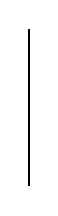
\begin{tikzpicture}
 \draw[thick,rounded corners=18pt]
(0,0) -- (0,2);    %  -- (1,3.25) -- (2,2) -- (2,0) -- (0,2) -- (2,2) -- (0,0) -- (2,0);
\end{tikzpicture}
\caption{You can draw lines of various thicknesses with tikz by using key value parameters.}
\end{figure}

The path starts at 0,0 the origin. You then continue from there.
\begin{figure}
\begin{tikzpicture}
 \draw[thick]
(0,0) -- (0,2)  -- (2,2);% -- (2,2) -- (2,0) -- (0,2) -- (2,2) -- (0,0) -- (2,0);
\end{tikzpicture}
\caption{You can draw lines of various thicknesses with tikz by using key value parameters.}
\end{figure}

We can draw an arrow by utilizing another style.
The path starts at 0,0 the origin. You then continue from there.
\begin{figure}
\begin{tikzpicture}
 \draw[->, thick]
(0,0) -- (0,2)  -- (2,2);% -- (2,2) -- (2,0) -- (0,2) -- (2,2) -- (0,0) -- (2,0);
\end{tikzpicture}
\caption{You can draw lines of various thicknesses with tikz by using key value parameters.}
\end{figure}


\section{Clipping}

\begin{tikzpicture}
\draw (0,0) circle (1cm);
\clip (0,0) circle (1cm);
\fill[black] (0cm,1cm) rectangle (-1cm,-1cm);
\end{tikzpicture}





\begin{tikzpicture}
\draw (0,0) circle (1cm);
\clip (0,0) circle (1cm);
\fill[black] (0cm,1cm) rectangle (-1cm,-1cm);
\end{tikzpicture}


\section{Beyond line segments}

In addition to points and line segments, there are a number of other graphic
primitives available. These include:

\begin{enumerate}
\item  Grids and rectangles
\item Circles and ellipses
\item  Arcs
\item  Bézier curves
\end{enumerate}

As previously discussed, a grid is specified by providing two diagonally opposing
points and other options which affect such things as the color and spacing of the
grid lines. A rectangle can be viewed as a simplified grid — all that is needed are
two diagonally opposing points of the rectangle. The syntax

backslash draw (P) rectangle (Q);

draws the rectangle specified by the two “bounding box” points P and Q. It is
worth noting that the current point is updated to Q, a fact which plays a role if
the backslash draw command involves more than one drawing action. Figure 14 provides
an example where three rectangles are drawn in succession. Each rectangle operation
updates the current point, which then serves as one of the bounding box
points for the following rectangle.

\begin{tikzpicture}
\draw [color=magenta](0,0) rectangle (1,1)
rectangle (3,2)
rectangle (4,3);
\end{tikzpicture}

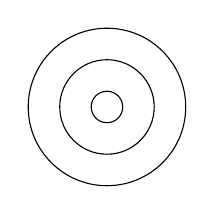
\begin{tikzpicture}
\draw (0,0) circle (1cm)
circle (0.6cm)
circle (0.2cm);
\end{tikzpicture}


\subsection{arcs}

Arcs are drawin in degrees, remember -- denotes a straight line, but in this case it rather denotes a connection.
\begin{verbatim}

\begin{tikzpicture}
\draw (0:1cm) -- (0:2cm)
arc (0:60:2cm) -- (60:1cm)
arc (60:0:1cm) -- cycle;
\end{tikzpicture}
\end{verbatim}

By using arc, we can generate arcs rather than circles. This can be quite useful.

\begin{figure}
\begin{center}

\begin{tikzpicture}
\draw (0:1cm) -- (0:2cm)
arc (0:60:2cm) -- (60:1cm)
arc (60:0:1cm) -- cycle;
\end{tikzpicture}
\caption{An arc drawn in a counterclock fashion}
\end{center}
\end{figure}

We can color the figure by using {\tt color=magenta}.

\begin{figure}
\begin{center}

\begin{tikzpicture}
\draw[color = magenta] (0:1cm) -- (0:2cm)
arc (0:60:2cm) -- (60:1cm)
arc (60:0:1cm) -- cycle;
\end{tikzpicture}
\caption{An arc drawn in a counterclock fashion}
\end{center}
\end{figure}

\section{From coordinates to nodes}

A node is a generalization of the coordinate primitive. Two characteristics of a
node are its shape and its text. A node allows for arbitrary TEX text to appear
within a diagram. The command


defines a node named v0, centered at the origin, with a circular shape and text
component $v_0$. The draw option causes the associated shape (in this case, a
circle) to be drawn. Figure 24 illustrates how nodes can be used to draw an undirected
graph. Notice how line segments which join nodes stop at the boundary

\begin{marginfigure}[5cm]
\begin{verbatim}
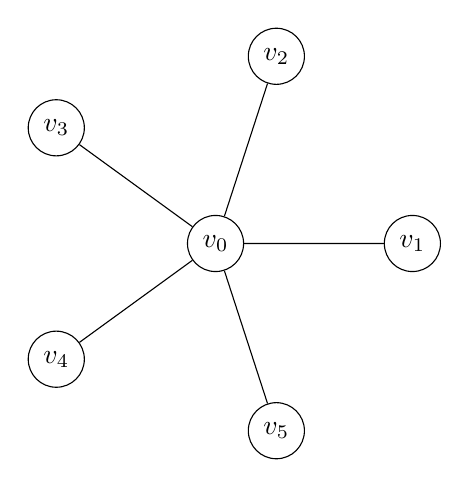
\begin{tikzpicture}[scale=2.5]
\tikzstyle{every node}=[draw,shape=circle];
\path (0:0cm) node (v0) {$v_0$};
\path (0:1cm) node (v1) {$v_1$};
\path (72:1cm) node (v2) {$v_2$};
\path (2*72:1cm) node (v3) {$v_3$};
\path (3*72:1cm) node (v4) {$v_4$};
\path (4*72:1cm) node (v5) {$v_5$};
\draw (v0) -- (v1)
(v0) -- (v2)
(v0) -- (v3)
(v0) -- (v4)
(v0) -- (v5);
\end{tikzpicture}
\end{verbatim}
\end{marginfigure}


\begin{center}
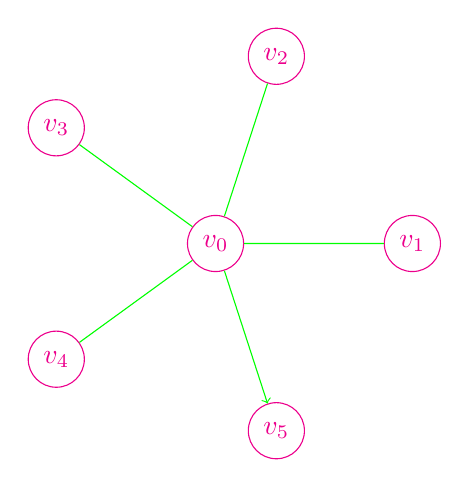
\begin{tikzpicture}[scale=2.5]
\tikzstyle{every node}=[draw,shape=circle, color=magenta];
\path (0:0cm) node (v0) {$v_0$};
\path (0:1cm) node (v1) {$v_1$};
\path (72:1cm) node (v2) {$v_2$};
\path (2*72:1cm) node (v3) {$v_3$};
\path [color=green] (3*72:1cm) node (v4) {$v_4$};
\path (4*72:1cm) node (v5) {$v_5$};
\draw [->, color=green] (v0) -- (v1)
(v0) -- (v2)
(v0) -- (v3)
(v0) -- (v4)
(v0) -- (v5);
\end{tikzpicture}
\end{center}


TikZ introduces a special syntax for adding text or, more generally, nodes to a graphic. When you specify
a path, add nodes as in the following example:
text

\begin{verbatim} \tikz \draw (1,1) node {text} -- (2,2); \end{verbatim}

Nodes are inserted at the current position of the path, but only after the path has been rendered. When
special options are given, as in draw (1,1) node[circle,draw] {text};, the text is not just put at the
current position. Rather, it is surrounded by a circle and this circle is "drawn."

You can add a name to a node for later reference either by using the option name=hnode namei or by
stating the node name in parentheses outside the text as in node[circle](name){text}.

Predefined shapes include rectangle, circle, and ellipse, but it is possible (though a bit challenging)
to define new shapes.

\section{Special Syntax for Specifying Trees}

In addition to the "node syntax,"  TikZ also introduces a special syntax for drawing trees. The syntax is
intergrated with the special node syntax and only few new commands need to be remebered. In essence, a
node can be followed by any number of children, each introduced by the keyword child. The children are
nodes themselves, each of which may have children in turn.
\begin{marginfigure}
\begin{verbatim}
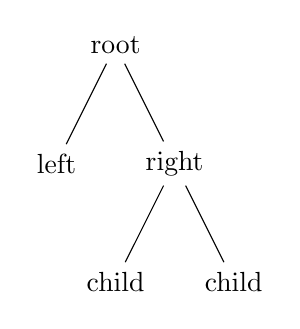
\begin{tikzpicture}
\node {root}
child {node {left}}
child {node {right}
child {node {child}}
child {node {child}}
};
\end{tikzpicture}
\end{verbatim}
\end{marginfigure}


\begin{figure}
\begin{center}
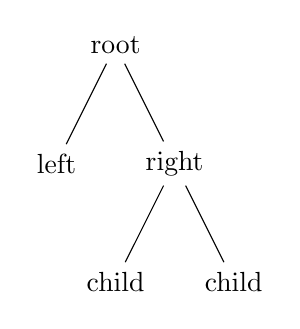
\begin{tikzpicture}
\node {root}
child {node {left}}
child {node {right}
child {node {child}}
child {node {child}}
};
\end{tikzpicture}
\end{center}
\end{figure}
Since trees are made up from nodes, it is possible to use options to modify the way trees are drawn. Here
are two examples of the above tree, redrawn with different options:

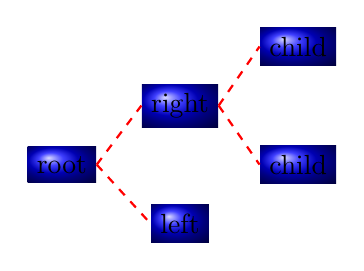
\begin{tikzpicture}
[parent anchor=east,child anchor=west,grow=east]
\tikzstyle{every node}=[ball color=blue, rectangle, text=black]
\tikzstyle{edge from parent}=[draw,dashed,thick,red]
\node {root}
child {node {left}}
child {node {right}
child {node {child}}
child {node {child}}
};
\end{tikzpicture}


Shading is accomplished by a style \tikz \shadedraw [shading=axis,shading angle=90] (0,0) rectangle (1,1);

\begin{figure}
\begin{center}
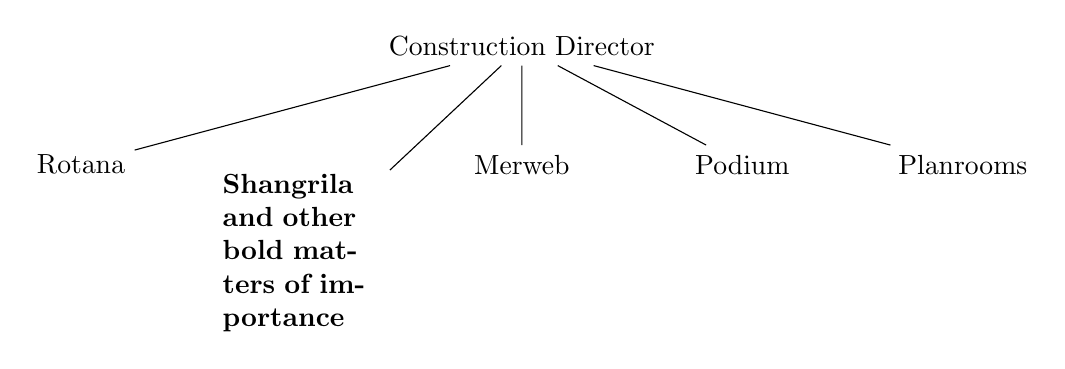
\begin{tikzpicture}

\tikzstyle{level 1}=[sibling distance=28mm]
\tikzstyle{level 2}=[sibling distance=30mm]
\tikzstyle{level 3}=[sibling distance=30mm]

\node {Construction Director}
child {node { Rotana}}
child {node [text width=2cm, anchor=north]{\bf Shangrila and other bold matters of importance}}
child{node {Merweb}}
child{node{Podium}}
child{node{Planrooms}};
\end{tikzpicture}
\end{center}
\end{figure}
\newpage

\chapter{Repeating Things}
\small
TikZ provides a loop structure which can simplify the creation of certain types of
graphics. The basic loop syntax is as follows:

\begin{verbatim}
\foreach \var in {iteration list}
   {
      loop body
    }
\end{verbatim}

The loop variable, {{\tt var}}, takes on the values given in the iteration list. In the
simplest case, this list can be a fixed list of values, such as {1,2,3,4} or as an
implied list of values, such as {1,...,4}.

Consider the loop in Figure 26. Four coordinates, X1 through X4 are introduced
at (1, 0), (2, 0), (3, 0), and (4, 0), respectively. In addition, a small filled
circle is drawn at each coordinate.

Figure 27 shows how to extend this idea to yield a bipartite graph. As one
might expect, foreach loops can be nested, a feature utilized here to specify all
the edges in the graph.

Iteration lists need not consist of consecutive integers. An implicit step size is
obtained by providing the first two values of the list in addition to the final value.






another test
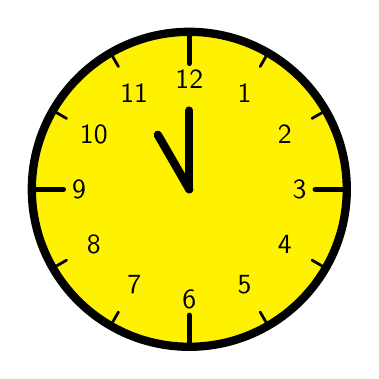
\begin{tikzpicture}[cap=round,line width=3pt]
\filldraw [fill=yellow] (0,0) circle (2cm);
\foreach \angle / \label in
{0/3, 30/2, 60/1, 90/12, 120/11, 150/10, 180/9,
210/8, 240/7, 270/6, 300/5, 330/4}
{
\draw[line width=1pt] (\angle:1.8cm) -- (\angle:2cm);
\draw (\angle:1.4cm) node{\textsf{\label}};
}
\foreach \angle in {0,90,180,270}
\draw[line width=2pt] (\angle:1.6cm) -- (\angle:2cm);
\draw (0,0) -- (120:0.8cm); % hour
\draw (0,0) -- (90:1cm); % minute
\end{tikzpicture}%

\tikz \fill[fill=yellow]
(0,0) node {first node}
-- (1,1) node  {second node}
-- (0,2) node {third node};

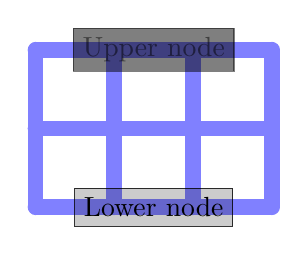
\begin{tikzpicture}
\draw[line width=2mm,blue!50,cap=round] (0,0) grid (3,2);
\tikzstyle{every node}=[fill,draw]
\node[opacity=0.5] at (1.5,2) {Upper node};
\node[draw opacity=0.8,fill opacity=0.2,text opacity=1]
at (1.5,0) {Lower node};
\end{tikzpicture}

\chapter{Paths}

\begin{pgfpicture}
\pgfpathmoveto{\pgfpointorigin}
\pgfpathlineto{\pgfpoint{1cm}{1cm}}
\pgfpathlineto{\pgfpoint{2cm}{1cm}}
\pgfpathlineto{\pgfpoint{3cm}{0.5cm}}
\pgfpathlineto{\pgfpoint{3cm}{0cm}}
\pgfsetfillcolor{red}
\pgfusepath{fill,stroke}
\end{pgfpicture}

check this one out for a while 


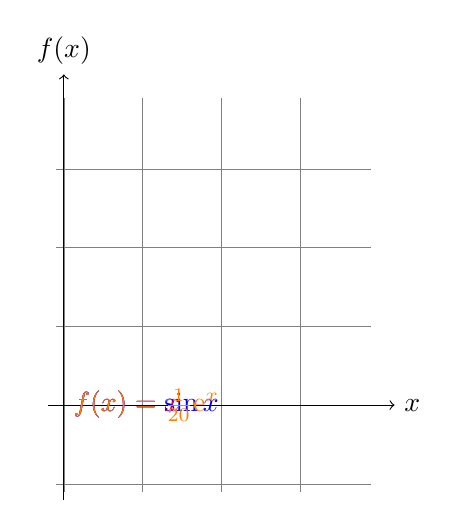
\begin{tikzpicture}[domain=0:4]
\draw[very thin,color=gray] (-0.1,-1.1) grid (3.9,3.9);
\draw[->] (-0.2,0) -- (4.2,0) node[right] {$x$};
\draw[->] (0,-1.2) -- (0,4.2) node[above] {$f(x)$};
\draw[color=red] plot[id=x] function{x} node[right] {$f(x) =x$};
\draw[color=blue] plot[id=sin] function{sin(x)} node[right] {$f(x) = \sin x$};
\draw[color=orange] plot[id=exp] function{0.05*exp(x)} node[right] {$f(x) = \frac{1}{20} \mathrm e^x$};
\end{tikzpicture}




 \chapter{Plotting}
\begin{figure}
% Preamble: \pgfplotsset{width=7cm,compat=1.3}
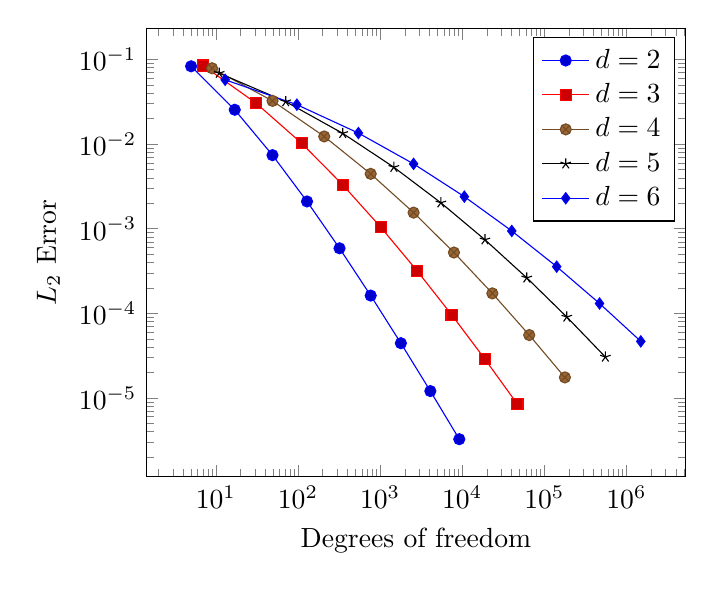
\begin{tikzpicture}
\begin{loglogaxis}[
xlabel={Degrees of freedom},
ylabel={$L_2$ Error}
]
\addplot coordinates {
(5,8.312e-02) (17,2.547e-02) (49,7.407e-03)
(129,2.102e-03) (321,5.874e-04) (769,1.623e-04)
(1793,4.442e-05) (4097,1.207e-05) (9217,3.261e-06)
};
\addplot coordinates{
(7,8.472e-02) (31,3.044e-02) (111,1.022e-02)
(351,3.303e-03) (1023,1.039e-03) (2815,3.196e-04)
(7423,9.658e-05) (18943,2.873e-05) (47103,8.437e-06)
};
\addplot coordinates{
(9,7.881e-02) (49,3.243e-02) (209,1.232e-02)
(769,4.454e-03) (2561,1.551e-03) (7937,5.236e-04)
(23297,1.723e-04) (65537,5.545e-05) (178177,1.751e-05)
};
\addplot coordinates{
(11,6.887e-02) (71,3.177e-02) (351,1.341e-02)
(1471,5.334e-03) (5503,2.027e-03) (18943,7.415e-04)
(61183,2.628e-04) (187903,9.063e-05) (553983,3.053e-05)
};
\addplot coordinates{
(13,5.755e-02) (97,2.925e-02) (545,1.351e-02)
(2561,5.842e-03) (10625,2.397e-03) (40193,9.414e-04)
(141569,3.564e-04) (471041,1.308e-04) (1496065,4.670e-05)
};
\legend{$d=2$,$d=3$,$d=4$,$d=5$,$d=6$}
\end{loglogaxis}

\end{tikzpicture}
\caption{A multiline graph}
\end{figure}

The beauty of this package is that we can use equations for plotting.


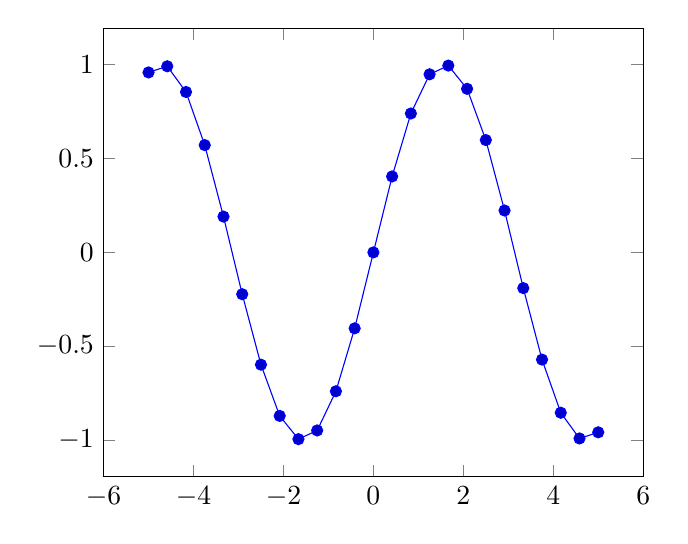
\begin{tikzpicture}
\begin{axis}
\addplot {sin(deg(x))};
\end{axis}
\end{tikzpicture}


\noindent We can draw two graphs one on top of each other by using some text in between. this will force \LaTeXe to float the figures better.


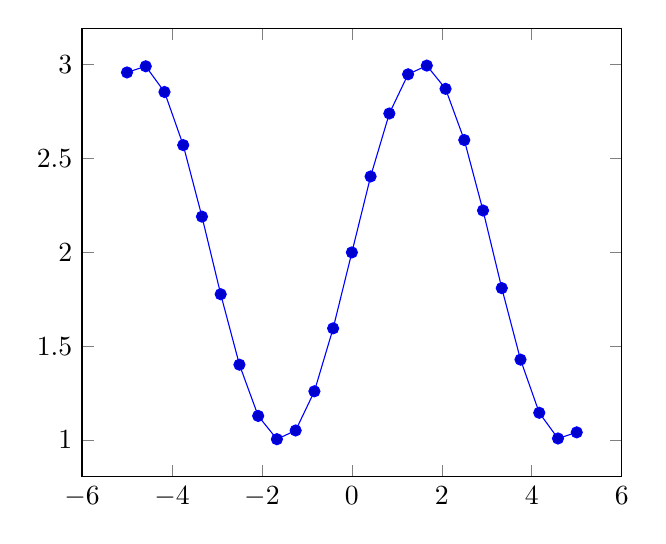
\begin{tikzpicture}
\begin{axis}
\addplot {sin(deg(x))+2}; %the + will only use the points
\end{axis}
\end{tikzpicture}

Using the Tufte book package we can place figures in the margin as well. This is very good.
\begin{marginfigure}
\pgfplotsset{width=4cm,compat=1.3}
\begin{tikzpicture}
\begin{axis}[
xlabel=Cost,
ylabel=Error]
\addplot[color=red,mark=x] coordinates {
(20,-2.8559703)
(3,-3.5301677)
(4,-4.3050655)
(5,-5.1413136)
(6,-6.0322865)
(7,-6.9675052)
(8,-7.9377747)
};
\end{axis}
\end{tikzpicture}
\end{marginfigure}

\begin{center}
\color{brown}{
\small{
\begin{verbatim}
           %\usepackage{ifthen}
          \newcommand{\weekday}[1]%
         {%
             \ifthenelse{\equal{#1}{1}}{Monday}{}%
             \ifthenelse{\equal{#1}{2}}{Tuesday}{}%
             \ifthenelse{\equal{#1}{3}}{Wednesday}{}%
             \ifthenelse{\equal{#1}{4}}{Thursday}{}%
             \ifthenelse{\equal{#1}{5}}{Friday}{}%
             \ifthenelse{\equal{#1}{6}}{Saturday}{}%
             \ifthenelse{\equal{#1}{7}}{Sunday}{}%
}

\weekday{3}

\end{verbatim}
}
}
\end{center}

\begin{tabular}{|lll}
\toprule
sl. & item & price\\
\midrule
1  & Butterfly valves & 23\\
\bottomrule
\end{tabular}





%\ctable[]{rlcc}{
\tnote{for the abstraction reaction,$\fam0 Mu+HX \rightarrow MuH+X$.}
\tnote[b]{1 degree${} = \pi/180$ radians.}
\tnote[c]{this is a particularly long note, showing that
footnotes are set in raggedright mode as we don't like
hyphenation in table footnotes.}
}{ \FL
& & $\fam0 H(Mu)+F_2$ & $\fam0 H(Mu)+Cl_2$ \ML
&$\beta$(H) & $80.9^\circ$\tmark[b] & $83.2^\circ$ \NN
&$\beta$(Mu) & $86.7^\circ$ & $87.7^\circ$ \LL
}


\ctable[]{c>{\raggedright}Xc>{\raggedright}X}{
\tnote{footnotes are placed under the table}
}{ \FL
\multicolumn{4}{c}{Example using tabularx} \ML
\multicolumn{2}{c}{Multicolumn entry!} & THREE & FOUR \NN
\cmidrule(r){1-2}\cmidrule(rl){3-3}\cmidrule(l){4-4}
one&
The width of this column depends on the width of the
table.\tmark &
three&
Column four will act in the same way as
column two, with the same width. \LL
}




\lstloadlanguages{Pascal, Ada}
\lstset{language=Pascal,commentstyle=\scriptsize}
A "for" loop in C:
\begin{lstlisting}[keywordstyle=\underbar]
int sum;
int i; /*for loop variable*/
sum=0;
for (i=0;i<n;i++) {
  sum += a[i];
}
\end{lstlisting}
Now the same loop in Ada:
\begin{lstlisting}[language=Ada]
Sum: Integer;
-- no decl for I necessary
Sum := 0;
for I in 1..N loop
Sum := Sum + A(I);
end loop;
\end{lstlisting}


\appendix{Common Requirements}
\section{Highlighting text}



\newenvironment{Description}
{\begin{list}{}{\let\makelabel\Descriptionlabel
\setlength\labelwidth{40pt}%
\setlength\leftmargin{\labelwidth+\labelsep}}}%
{\end{list}}
\newcommand*\Descriptionlabel[1]{\textsf{#1:}\hfil}
\begin{Description}
\item[Description]
Returns from a function. If issued at top level,
the interpreter simply terminates, just as if
end of input had been reached.
\item[Errors] None.
\item[Return values]
\mbox{}\\
Any arguments in effect are passed back to the
caller.
\end{Description}


\chapter{Multicolumn Layouts}
\begin{multicols}{2}
Here is some text to be distributed over
several columns. 
narrow try typesetting ragged right.
\lipsum
\end{multicols}

\chapter{Climate}
The variations in temperature, humidity and wind occurring throughout the world are due
to several factors the integration of which, for a particular locality, provides the climate
experienced. There is, first, a seasonal change in climatic conditions, varying with latitude
and resulting from the fact that, because the earth's axis of rotation is tilted at about 23.5 ~
to its axis of revolution about the sun, the amount of solar energy received at a particular
place on the earth's surface alters throughout the year. The geography of the locality
provides a second factor, influential in altering climate within the confines imposed by the
seasonal variation.

Figure 5.1 illustrates the geometrical considerations which show that, at a particular
latitude, the earth receives less solar radiation in winter than it does in summer. The
importance of this in its effect on the seasons stems from the fact that, for all practical
purposes, the sun is the sole supplier of energy to the earth.

The geography of a place determines how much solar energy is absorbed by the earth,
how much is stored and how readily it is released to the atmosphere. The atmosphere is
comparatively transparent to the flux of radiant solar energy (termed \emph{insolation\/}) but the
land masses which receive the energy are opaque to it and are fairly good absorbers of it,
although this depends on the reflectivity of the surface. This means that the thermal energy
from the sun warms up land surfaces on which it falls. Some of this energy travels inwards
and is stored in the upper layers of the earth's crust; some is convected to the atmosphere
and some is re-radiated back to space, but at a longer wavelength (about 10 micrometres),
since its mean surface temperature is very much less than that of the sun. Four-fifths of the
earth's surface is water, not land, and water behaves in a different fashion as a receiver of
insolation, being partially transparent to it; consequently, the energy is absorbed by the
water in depth, with the result that its surface temperature does not reach such a high value
during the daytime. On the other hand, at night, heat is lost from the land to the sky much
more rapidly since less was stored in its shallow upper crust than was absorbed and stored
in the deeper layers of water. The result is that land-surface temperatures tend to be lower
at night than are water-surface temperatures. It is evident from this that places in the
middle of large land masses will tend to have a more extreme annual variation of temperature
than will islands in a large sea. Thus, the climate of places on the same latitude can vary
enormously. To realise this we have but to compare the temperate seasons experienced in
the British Isles with the extremes suffered in Central Asia and Northern Canada at about
the same latitude. The exchanges of radiant energy cited above as responsible for the
differences in maritime and continental climates are complicated somewhat by the amount
of cloud. Cloud cover acts as an insulating barrier between the earth and its environment;
not only does it reflect back to outer space a good deal of the solar energy incident upon
it but it also stops the passage of the low-frequency infra-red radiation which the earth
emits. In addition, the quantity of carbon dioxide in the atmosphere reduces the emission
of infra-red radiation. Mountain ranges also play a part in altering the simple picture,
presented above, of a radiation balance.


The effect of the unequal heating of land and sea is to produce air movement. This air
movement results in adiabatic expansions and compressions taking place in the atmosphere,
with consequent decreases and increases respectively in air temperature. These temperature
changes, in turn, may result in cloud formation as values below the dew point are reached.
One overall aspect of the thermal radiation balance is prominent in affecting our weather
and in producing permanent features of air movement such as the Trade Winds and the
Doldrums. This is the fact that, for higher latitudes, the earth loses more heat to space by
radiation than it receives from the sun but, for lower latitudes, the reverse is the case. The
result is that the lower latitudes heat up and the higher ones cool down. This produces a
thermal up-current from the equatorial regions and a corresponding down-current in the
higher latitudes. While this is true for an ideal atmosphere, the fact that the earth rotates
and that other complicating factors are present means that the true behaviour is quite
involved and not yet fully understood.


\section{ Winds}
It might be thought that wind flowed from a region of high pressure to one of low pressure,
following the most direct path. This is not so. There are, in essence, three things which
combine to produce the general pattern of wind flow over the globe. This pattern is
complicated further by local effects such as the proximity of land and sea, the presence of
mountains and so on. However, the three overall influences are:


(i) the unequal heating of land and sea;

(2)the deviation of the wind due to forces arising from the rotation of the earth about its
axis;
(iii) the conservation of angular momentum~a factor occurring because the linear velocity
of air at low latitudes is less than at high latitudes.
The general picture of wind distribution is as follows. Over equatorial regions the weather
is uniform; the torrid zone is an area of very light and variable winds with frequent calms,
cloudy skies and violent thunderstorms. These light and variable winds are called the
'Doldrums'. Above and below the Doldrums, up to 30 ~ north and south, are the Trade
Winds, which blow with considerable steadiness, interrupted by occasional storms. Land
and sea breezes (mentioned later) also affect their behaviour.

Above and below 30 ~ of latitude, as far as the sub-polar regions, the Westerlies blow.
They are the result of the three factors mentioned earlier, but their behaviour is very much
influenced by the development of regions of low pressure, termed cyclones, producing
storms of the pattern familiar in temperate zones. This cyclonic influence means that the
weather is much less predictable in the temperate zones, unless the place in question is in
a very large land mass--for example in Asia or in North America. In temperate areas
consisting of a mixture of islands, broken coastline and sea, as in north-western Europe,
cyclonic weather is the rule and long-term behaviour difficult to forecast. The whole
matter is much complicated by the influence of warm and cold currents of water.

\section{Mist and fog}
For condensation to occur in the atmosphere the presence is required of small, solid
particles termed condensation nuclei. Any small solid particle will not do; it is desirable
that the particles should have some affinity for water. Hygroscopic materials such as salt
and sulphur dioxide then, play some part in the formation of condensation. The present
opinion appears to be that the products of combustion play an important part in the provision
of condensation nuclei and that the size and number of these nuclei vary tremendously.

Over industrial areas there may be several million per cubic centimetre of air whereas, over
sea, the density may be as low as a few hundred per cubic centimetre.

These nuclei play an important part in the formation of rain as well as fog, but for fog
to form the cooling of moist air must also take place. There are two common sorts of fog:

advection fog, formed when a moist sea breeze blows inland over a cooler land surface,
and radiation fog. Radiation fog forms when moist air is cooled by contact with ground
which has chilled as the result of heat loss by radiation to an open sky. Cloud cover
discourages such heat loss and, inhibiting the fall of surface temperature, makes fog formation
less likely. Still air is also essential; any degree of wind usually dissipates fog fairly
rapidly. Fog has a tendency to occur in the vicinity of industrial areas owing to the local
atmosphere being rich in condensation nuclei. Under these circumstances, the absence of
wind is helpful in keeping up the concentration of such nuclei. The dispersion of the nuclei
is further impeded by the presence of a temperature inversion, that is, by a rise in air
temperature with increase of height, instead of the reverse. This discourages warm air from
rising and encourages the products of combustion and fog to persist, other factors being
helpful.

Long-wave thermal radiation, ILW, directed to the sky at night can be considered as
radiation to a black body at a temperature of absolute zero. This is modified by a correction
factor to account for variations in the absorption by water vapour in the lower reaches of
the atmosphere. This changes as the amount of cloud cover and the area of the sky seen by
the surface varies. According to Brunt (1932) the absorption effect can be accounted for by
a vapour correction factor, $K$, expressed by

\begin{equation}
K = 0.56 - 0.08 \sqrt{p_s}
\end{equation}

where Ps is the vapour pressure of the air in millibars. The amount of sky seen by a surface
is given by an angle factor, B,

\begin{equation}
B = 0.5(1 + \cos \delta)
\end{equation}

where $\delta$  is the acute angle between the surface and the horizontal. Thus for a flat roof 8 =
0 and B = 1, whereas for a wall 8 = 90 ~ and B = 0.5. Cloud cover can play a part as well
and if we assume it is wholly effective in suppressing loss from the surface to outer space,
a cloud cover factor, C, can be introduced. Table 5.1 gives typical, approximate, average
cloud cover factors for Kew, based on data recorded for the amount of bright sunshine
received between sunrise and sunset in relation to the maximum amount of sunshine that
could be received during the same period of the day.

\begin{minipage}{5in}
\begin{tabular}{lllllllllllll}
\toprule
Month &Jan &Feb &Mar &Apr &May &Jun &Jul &Aug &Sep &Oct &Nov &Dec\\
\midrule
C &0.2 &0.2   &0.3   &0.4   &0.4  &0.4  &0.4  &0.4  &0.4  &0.3 &0.2 &0.2\\
\bottomrule
\end{tabular}
\end{minipage}
\def\badcheck{A penalty has been added because your
check to us was not honored by your bank.\par}
\def\cheater{A penalty of 50\% of the underpaid tax
has been added for fraud.\par}

\chapter{Solar Heat gains}

\section{The composition of heat gains}

Heat gains are either sensible, tending to cause a rise in air temperature, or latent, causing
an increase in moisture content. In comfort air conditioning sensible gains originate from
the following sources:

(i) Solar radiation through windows, walls and roofs.

(ii) Transmission through the building envelope and by the natural infiltration of warmer
air from outside.

(iii) People.

(iv) Electric lighting.


Latent heat gains are due to the presence of the occupants and the natural infiltration of
more humid air from outside.

In the case of industrial air conditioning there may be additional sensible and latent heat
gains from the processes carried out.

All the above sources of heat gain are well researched but a measure of uncertainty is
introduced by the random nature of some, such as the varying presence of people and the
way in which electric lights are switched. The thermal inertia of the building structure also
introduces a problem when calculating the sensible heat gain arising from solar radiation.
It follows that a precise determination of heat gains is impossible. Nevertheless, it is vital
that the design engineer should be able to calculate the heat gains with some assurance and
this can be done when generally accepted methods of calculation are followed, supported
by sound common sense. The following text discusses and describes such methods.


\section{The physics of solar radiation}

The sun radiates energy as a black body having a surface temperature of about 6000°C
over a spectrum of wavelengths from 300 to 470 nm. Nine per cent of the energy is in the
ultra-violet region but 91 per cent of the energy is in the visible part of the spectrum (380-
780 nm) and in the infra-red. Figure 7.1 shows a typical spectral distribution of the energy
reaching the surface of the earth. The peak intensity of the solar energy reaching the upper
limits of the atmosphere of the earth is about 2200 W mV2 at 480 nm but the average total
termed the \emph{solar constant}, is 1367  $W\/  m^{-2}$ \sidenote{Use SI units for consistency}, according to Iqbal(1983). The orbit of the earth
about the sun is an ellipse and the earth is slightly closer to the sun in January than it is in
July. Consequently the solar irradiation\index{solar irradiation}  has a maximum value of 1413 W mP2 in January
and a minimum of 1332 W m-2 in July.

A total of only about 1025 W m-2 reaches the surface of the earth when the sun is
vertically overhead in a cloudless sky. Of this figure, about 945 W m-2  is by radiation
received directly from the sun, the remainder being solar radiation received indirectly from
the sky.



\begin{verbatim}


S0573	Arvind Kumar Sing	Senior Mech. Design Engineer	3464665	     a.singh@habtoorspecon.com	
S0731	Jabir Chakkumpurauil	Mech. Design Engineer	7066351		Design
S0759	Safwan Abdussalam	Mech. Design Engineer	7066351		Design
S0797	Satheesh Kumar Puthen	Mechanical Engineer	7875093		HVAC-B3 LV1
Sobhi Qussini	Mechanical Engineer	5343343		Quantities


S0725	Satish Pai Kasturi	Mechanical Engineer	3474506		Design
S0775	Venchito Cortez Galvez	Mechanical Engineer	3682788		Bob
S0801	Moideen Kunhi Kallikatte	Mechanical Engineer	5038861		Plantrooms
S0295	Bernabe Jr Urdaneta Orbeso	Mechanical Engineer Project	3251084   o.bernabe@habtoorspecon.com	
S0477	Deepash Lal	Mechanical Engineer	3449230		Rotana
S0569	Ritzie Argota	Mechanical Engineer	3458542	r.argota@habtoorspecon.com	
S0754	Jeffrey Magaoay	Mechanical Engineer	3171978	j.magaoay@habtoorspecon.com	Fire Fighting B3-LV7

S0742	Velmurugan Annamalai	Mechanical Engineer Site 	3482758		Podium?
S0289	Sripathy Nagaraj	Mechanical Engineer	3297515	sripathy@habtoorspecon.com

%S0726	Gautham Raj	Mechanical Engineer	3560349	g.raj@habtoorspecon.com	Procurement Dept.
%S0297	Sita Rambabu Bommu	Mechanical Engineer	3188697	b.sitarambabu@habtoorspecon.com	Procurement Dept.


1	S0723	Taha Mahmoud Taha Ammar	Electrical Engineer Project	6233226	t.ammar@habtoorspecon.com	Design
2	S0679	Chockalingam Sampath	Senior Elec. Design Engineer	3474371	c.sam@habtoorspecon.com	Design
3		Gelenn Completo Mahtani	Elec. Design Engineer	6641125		Design
4	S0252	Franklin Tamayo Canoy	Electrical Engineer	3254369	f.canoy@habtoorspecon.com	Procurement Dept.
5	S0285	Martiniano Lompot Tan	Electrical Engineer	5114319	bob	
6	S0286	Pedro Jr. Zacarias Reyes	Electrical Engineer	5119516	p.reyes@habtoorspecon.com	Nidal
7	S0653	Rahul Krishnan	Electrical Engineer	3472693		
8		Amirhosein Tavanfar	Electrical Engineer	6986499		
9		Saudi Ghassan	Electrical Engineer	5025781		
10	S0300	Soloman Alphonse	Electrical Engineer Assistant	5685518		
11		Hamza Omar Ibrahim Al-Far	Site.Electrical Engineer	3693637		

1	S0494	Armin Alrvarez	Sr.Planing Engineer	3265313	a.alvarez@habtoorspecon.com	PLANNING
2	S0709	Enamuthu Sankaran	Planning Engineer	3517732		PLANNING
5	S0675	Jashvantkumar Patel	Sr. QA/QC Engineer	3543627	j.patel@habtoorspecon.com	QA
3	S0298	Justo Laconsay Caliguiran	QA/QC Engineer	5929833	j.calliguran@habtoorspecon.com	QA
4	S0743	Mohammed Siyas	QA/QC Engineer	3485607		QA


\end{verbatim}
%% Example
%% 
   
   \out{Close Ceilings Rotana Floor 10}{Line 2}
   \out{Rotana,  power-on}{12$^{th}$ Sept 2010}
   \out{Rotana Qatar Cool switch-on}{12th September}


%% we now read the file and dostuff with it
%% 
\chapter{Summary of  Key Dates}
\immediate\closeout\tempfile
\keydate { Naffco Controllers}{30 January 2013}
\keydate { Rotana kitchen extract}{25 Feb 2013}
\keydate { Shangri-la kitchen extract}{15 Mar 2013}
\keydate { Merweb kitchen extract}{30 Mar 2013}




\backmatter
%\bibliography{sample-handout}
%\bibliographystyle{plainnat}
\printindex



%% finally we close the file
%%




\end{document}
